\documentclass[twoside]{book}

% Packages required by doxygen
\usepackage{fixltx2e}
\usepackage{calc}
\usepackage{doxygen}
\usepackage[export]{adjustbox} % also loads graphicx
\usepackage{graphicx}
\usepackage[utf8]{inputenc}
\usepackage{makeidx}
\usepackage{multicol}
\usepackage{multirow}
\PassOptionsToPackage{warn}{textcomp}
\usepackage{textcomp}
\usepackage[nointegrals]{wasysym}
\usepackage[table]{xcolor}

% Font selection
\usepackage[T1]{fontenc}
\usepackage[scaled=.90]{helvet}
\usepackage{courier}
\usepackage{amssymb}
\usepackage{sectsty}
\renewcommand{\familydefault}{\sfdefault}
\allsectionsfont{%
  \fontseries{bc}\selectfont%
  \color{darkgray}%
}
\renewcommand{\DoxyLabelFont}{%
  \fontseries{bc}\selectfont%
  \color{darkgray}%
}
\newcommand{\+}{\discretionary{\mbox{\scriptsize$\hookleftarrow$}}{}{}}

% Page & text layout
\usepackage{geometry}
\geometry{%
  a4paper,%
  top=2.5cm,%
  bottom=2.5cm,%
  left=2.5cm,%
  right=2.5cm%
}
\tolerance=750
\hfuzz=15pt
\hbadness=750
\setlength{\emergencystretch}{15pt}
\setlength{\parindent}{0cm}
\setlength{\parskip}{3ex plus 2ex minus 2ex}
\makeatletter
\renewcommand{\paragraph}{%
  \@startsection{paragraph}{4}{0ex}{-1.0ex}{1.0ex}{%
    \normalfont\normalsize\bfseries\SS@parafont%
  }%
}
\renewcommand{\subparagraph}{%
  \@startsection{subparagraph}{5}{0ex}{-1.0ex}{1.0ex}{%
    \normalfont\normalsize\bfseries\SS@subparafont%
  }%
}
\makeatother

% Headers & footers
\usepackage{fancyhdr}
\pagestyle{fancyplain}
\fancyhead[LE]{\fancyplain{}{\bfseries\thepage}}
\fancyhead[CE]{\fancyplain{}{}}
\fancyhead[RE]{\fancyplain{}{\bfseries\leftmark}}
\fancyhead[LO]{\fancyplain{}{\bfseries\rightmark}}
\fancyhead[CO]{\fancyplain{}{}}
\fancyhead[RO]{\fancyplain{}{\bfseries\thepage}}
\fancyfoot[LE]{\fancyplain{}{}}
\fancyfoot[CE]{\fancyplain{}{}}
\fancyfoot[RE]{\fancyplain{}{\bfseries\scriptsize Generated by Doxygen }}
\fancyfoot[LO]{\fancyplain{}{\bfseries\scriptsize Generated by Doxygen }}
\fancyfoot[CO]{\fancyplain{}{}}
\fancyfoot[RO]{\fancyplain{}{}}
\renewcommand{\footrulewidth}{0.4pt}
\renewcommand{\chaptermark}[1]{%
  \markboth{#1}{}%
}
\renewcommand{\sectionmark}[1]{%
  \markright{\thesection\ #1}%
}

% Indices & bibliography
\usepackage{natbib}
\usepackage[titles]{tocloft}
\setcounter{tocdepth}{3}
\setcounter{secnumdepth}{5}
\makeindex

% Hyperlinks (required, but should be loaded last)
\usepackage{ifpdf}
\ifpdf
  \usepackage[pdftex,pagebackref=true]{hyperref}
\else
  \usepackage[ps2pdf,pagebackref=true]{hyperref}
\fi
\hypersetup{%
  colorlinks=true,%
  linkcolor=blue,%
  citecolor=blue,%
  unicode%
}

% Custom commands
\newcommand{\clearemptydoublepage}{%
  \newpage{\pagestyle{empty}\cleardoublepage}%
}

\usepackage{caption}
\captionsetup{labelsep=space,justification=centering,font={bf},singlelinecheck=off,skip=4pt,position=top}

%===== C O N T E N T S =====

\begin{document}

% Titlepage & ToC
\hypersetup{pageanchor=false,
             bookmarksnumbered=true,
             pdfencoding=unicode
            }
\pagenumbering{alph}
\begin{titlepage}
\vspace*{7cm}
\begin{center}%
{\Large A\+ID Coding Challenge -\/ The Bachelor }\\
\vspace*{1cm}
{\large Generated by Doxygen 1.8.14}\\
\end{center}
\end{titlepage}
\clearemptydoublepage
\pagenumbering{roman}
\tableofcontents
\clearemptydoublepage
\pagenumbering{arabic}
\hypersetup{pageanchor=true}

%--- Begin generated contents ---
\chapter{A\+ID Coding Challenge Solution}
\label{index}\hypertarget{index}{}This is my solution for the A\+ID Bachelor Coding Challenge. For the problem description refer to the A\+ID \href{../../AID Coding Challenge.pdf}{\tt Coding Challenge.\+pdf}. The complete doxygen documentation can be found in the doc folder.

\section*{Result}

Travelling from the Rover (R\+O\+V\+E\+R\+\_\+X, R\+O\+V\+E\+R\+\_\+Y) to the Bachelor (B\+A\+C\+H\+E\+L\+O\+R\+\_\+X, B\+A\+C\+H\+E\+L\+O\+R\+\_\+Y) will take 2094.\+51 island seconds (34.\+9085 island minutes or 0.\+581809 island hours) on the shortest path.

Travelling from the Bachelor (B\+A\+C\+H\+E\+L\+O\+R\+\_\+X, B\+A\+C\+H\+E\+L\+O\+R\+\_\+Y) to the Wedding (W\+E\+D\+D\+I\+N\+G\+\_\+X, W\+E\+D\+D\+I\+N\+G\+\_\+Y) will take 1283.\+17 island seconds (21.\+3862 island minutes or 0.\+356436 island hours) on the shortes path.



\section*{Algorithm Choice}

To find the fastest route from a start to a goal location, I considered Gradient Fields, Dynamic Programming and Graph Search. I decided for A$\ast$ graph search algorithm, which uses Dynamic Programming to find the shortest path. Compared to Dijkstra it utilizes a heuristic $h(n)$ which provides an estimate of the minimum cost from any node n to the goal.

Looking at the map, I deceided against Gradient because of the non convex constraints that are imposed by the fjords.

\subsection*{Cost Function}

The evaluation function $f(n) = g(n) + h(n)$ describes the total cost of a node. It consists of the path cost $g(n)$, which describes how long it takes the rover to get to node $n$ from its start location.

The path cost $g(n)$ is calculated using the parent node\textquotesingle{}s path cost $g(parent)$ and the step cost $c(n)$, which is the cost of getting from the parent to the current node. The step cost is described in the next section \mbox{\hyperlink{index_step-cost}{step-\/cost}}.

Because the robot can move in eight directions (straight and diagonal) I use an octile distance heuristic $h(n)$, implemented in c\+Planner\+::\+Update\+Heuristic(). To get a consistent heuristic, I scaled it using the maximum gradient analyzing the elevation of the map and taking the slope into account. The consistency $ h(n) <= c(n,p) + h(p)$ is checked in planner\+::c\+Planner\+::\+Heuristic\+Check(). I exported the calculated heuristic values using \mbox{\hyperlink{classplanner_1_1c_planner_a1a4650050656545744796296a653d388}{planner\+::c\+Planner\+::\+Generate\+Heuristic()}} in the google test T\+E\+S\+T\+\_\+\+F(c\+Planner\+Test, heuristic) (see, test\+\_\+system.\+cpp).



\subsection*{Step Cost Model}\hypertarget{index_step-cost}{}\section{step-\/cost}\label{index_step-cost}
Another task was to model the speed of the rover when driving up or downhill. For this I implemented a simple kinematic approach with an inclined plane to model the elevation.





The first step is to calculate the descent or ascent using the height difference between two locations, see \mbox{\hyperlink{classplanner_1_1c_planner_a82e45fc2701e90d3fa9df72f475e455e}{planner\+::c\+Planner\+::\+Update\+Cost()}}. In this method the pitch angle is calculated next, followed by computing the x component of the downhill-\/slope force using the gravitational force $F_G$.

\begin{eqnarray*} F_H &= F_G \cdot sin\alpha \rightarrow a = g \cdot sin\alpha \\ F_{H,x} &= a \end{eqnarray*}

The rover’s speed is lower uphill. It’s part of the task to model in which way it becomes slower.  The rover’s speed gets higher when running downhill. It’s part of the task to model in which way it becomes faster.

\section*{Time and Space Complexity}

I tried to avoid alocating two dimensional vectors of the image size. Instead I am using a std\+::priority\+\_\+queue \mbox{\hyperlink{priority__queue_8h_source}{priority\+\_\+queue.\+h}} (planner\+::c\+Planner\+::m\+\_\+po\+Frontier) and a std\+::map. The priority queue is sorted by the score value of the evaluation function $f(n)$.

\section*{Software Organization and Architecture}\hypertarget{index_software}{}\section{software}\label{index_software}
The advantage of using interfaces is to get different implementations with different behavior but keep the public interface methods the same. I use two interfaces that reference each other, \mbox{\hyperlink{classplanner_1_1c_rover_interface}{planner\+::c\+Rover\+Interface}} and \mbox{\hyperlink{classplanner_1_1c_planner_interface}{planner\+::c\+Planner\+Interface}}. The \mbox{\hyperlink{classplanner_1_1c_audi_rover}{planner\+::c\+Audi\+Rover}} implements \mbox{\hyperlink{classplanner_1_1c_rover_interface}{planner\+::c\+Rover\+Interface}} and acts as a factory, creating \mbox{\hyperlink{classplanner_1_1c_planner}{planner\+::c\+Planner}} in planner\+::c\+Rover\+Interface\+::\+Initialize\+Planner(). To start planning the start and goal positions of the rover need to be set, planner\+::c\+Rover\+Interface\+::\+Set\+Start() and planner\+::c\+Rover\+Interface\+::\+Set\+Goal() passing a location struct of type t\+Location. After the initialization, a call to the method \mbox{\hyperlink{classplanner_1_1c_audi_rover_a52c48afa0829f858c19d3ecf4940db21}{planner\+::c\+Audi\+Rover\+::\+Summon()}} invokes the planner\+::c\+Planner\+Interface\+::\+Plan(). Possible parameters to \mbox{\hyperlink{classplanner_1_1c_audi_rover_a52c48afa0829f858c19d3ecf4940db21}{planner\+::c\+Audi\+Rover\+::\+Summon()}} are the step size planner\+::c\+Rover\+Interface\+::m\+\_\+n\+Step\+Size and its velocity planner\+::c\+Rover\+Interface\+::m\+\_\+n\+Velocity (not tested \mbox{\hyperlink{index_testing}{testing}}).

\section*{Coding Style}

For the variable naming conventions, I follow the \href{https://en.wikipedia.org/wiki/MISRA_C}{\tt M\+I\+S\+RA C} standard.

\section*{Testing}\hypertarget{index_testing}{}\section{testing}\label{index_testing}
Note The tests are not completely finished because of the limited time.

I added google g\+Test version 1.\+8.\+0 to the zip file and created a test fixture \mbox{\hyperlink{classc_planner_test}{c\+Planner\+Test}} in \mbox{\hyperlink{test__fixture_8h_source}{test\+\_\+fixture.\+h}}. It is used to initialize the test by loading the evaluation.\+data and overrides.\+data files. Furthermore, the c\+Audi\+Rover is initialized in the \mbox{\hyperlink{classc_planner_test_a88ad8b0e63c66a9d94c7606aa67ef20d}{c\+Planner\+Test\+::\+Set\+Up}} method.

As explained in \mbox{\hyperlink{index_software}{software}} the default values for step size and velocity are set to one for both parameters. I tested with different step sizes to reach the goal faster, thereby verifying that the path and island seconds stay the same.

To get intermediate paths from the planner\+::c\+Planner\+::\+A\+Star() I used the provided visualizer\+::write\+B\+M\+P() inside A\+Star(). This results in the following output\+:

\section*{References}

\begin{DoxyItemize}
\item Artificial Intelligence A Modern Approach Third Edition -\/ Stuart Russel, Peter Norvig \item Head First Design Patterns -\/ Eric Freeman, Elisabeth Robson \item \href{https://autonomous-driving.org/2018/08/15/so-you-want-to-be-a-self-driving-car-engineer/}{\tt https\+://autonomous-\/driving.\+org/2018/08/15/so-\/you-\/want-\/to-\/be-\/a-\/self-\/driving-\/car-\/engineer/} \item \href{https://www.linkedin.com/pulse/software-quality-sami-vaaraniemi/}{\tt https\+://www.\+linkedin.\+com/pulse/software-\/quality-\/sami-\/vaaraniemi/} \item \href{https://en.wikipedia.org/wiki/A}{\tt https\+://en.\+wikipedia.\+org/wiki/A}$\ast$\+\_\+search\+\_\+algorithm \item \href{https://en.wikipedia.org/wiki/Consistent_heuristic}{\tt https\+://en.\+wikipedia.\+org/wiki/\+Consistent\+\_\+heuristic} \item \href{https://en.wikipedia.org/wiki/Admissible_heuristic}{\tt https\+://en.\+wikipedia.\+org/wiki/\+Admissible\+\_\+heuristic} \item \href{https://www.redblobgames.com/pathfinding/a-star/introduction.html}{\tt https\+://www.\+redblobgames.\+com/pathfinding/a-\/star/introduction.\+html} \end{DoxyItemize}

\chapter{A\+ID Coding Challenge Solution version 0.0.0}
\label{md___users_fjp_git_bachelor__r_e_a_d_m_e_v0}
\Hypertarget{md___users_fjp_git_bachelor__r_e_a_d_m_e_v0}
This is my solution for the A\+ID Bachelor Coding Challenge. For the problem description refer to the \href{AID_Coding_Challenge.pdf}{\tt A\+ID Coding Challenge.\+pdf}. The complete doxygen documentation can be found in the doc folder, see \href{doc/html/index.html}{\tt index.\+html}

\section*{Result Preview}

Travelling from the Rover (R\+O\+V\+E\+R\+\_\+X, R\+O\+V\+E\+R\+\_\+Y) to the Bachelor (B\+A\+C\+H\+E\+L\+O\+R\+\_\+X, B\+A\+C\+H\+E\+L\+O\+R\+\_\+Y) will take 2094.\+51 island seconds (34.\+9085 island minutes or 0.\+581809 island hours) on the fastest path.

Travelling from the Bachelor (B\+A\+C\+H\+E\+L\+O\+R\+\_\+X, B\+A\+C\+H\+E\+L\+O\+R\+\_\+Y) to the Wedding (W\+E\+D\+D\+I\+N\+G\+\_\+X, W\+E\+D\+D\+I\+N\+G\+\_\+Y) will take 1283.\+17 island seconds (21.\+3862 island minutes or 0.\+356436 island hours) on the fastest path.

In total the Audi rover requires 3377.\+68 island seconds (56.\+2947 island minutes or 0.\+938245 island hours) on the fastest path. Details are explained at the end in section Results. To plot the path I added another path() function to the visualizer.\+cpp.

image html solution\+\_\+rover\+\_\+bachelor\+\_\+wedding.\+jpg





\section*{Algorithm Choice}

To find the fastest route from a start to a goal location, I considered Gradient Fields, Dynamic Programming and Graph Search algorithms. I decided to use A$\ast$ graph search because it is an informed search algorithm, which uses a heuristic function $h(n)$ and relies on dynamic programming to find the shortest path. Compared to Dijkstra, which is an uninformed algorithm. The heuristic provides A$\ast$ ~\newline
 with an estimate of the minimum cost from any node n to the goal.

Another reason against Gradient descent are the non-\/convex constraints imposed by the fjords. Gradient descent could easily fall into a lokal minimum and get stuck, which would require methods such as stochastic gradient descent.

\subsection*{Cost Function}

The evaluation function $f(n) = g(n) + h(n)$ describes the total cost of a node. It consists of the path cost $g(n)$, which describes how long it takes the rover to get to node $n$ from its start location.

The path cost $g(n)$ is calculated using the parent node\textquotesingle{}s path cost $g(parent)$ and the step cost $c(n)$, which is the cost of getting from the parent to the current node and that has to be positive. The step cost is described in the next section step-\/cost.

In this challenge the heuristic represents the time it takes the robot to move from a node to the goal. Because the robot can move in eight directions (straight and diagonal) I use an octile distance heuristic $h(n)$, implemented in c\+Planner\+::\+Update\+Heuristic(). To get a consistent heuristic, I scaled it using the maximum gradient analyzing the elevation of the map and taking the slope into account. The consistency $ h(n) <= c(n,p) + h(p)$ is checked in \mbox{\hyperlink{classplanner_1_1c_planner_a1234d075676fcaa2c17b859d11b4638c}{planner\+::c\+Planner\+::\+Heuristic\+Check()}}. I exported the calculated heuristic values using \mbox{\hyperlink{classplanner_1_1c_planner_a1a4650050656545744796296a653d388}{planner\+::c\+Planner\+::\+Generate\+Heuristic()}} in the google test T\+E\+S\+T\+\_\+\+F(c\+Planner\+Test, heuristic) (see, test\+\_\+system.\+cpp).

image html heuristic.\+jpg



\subsection*{Step Cost Model}

Another task was to model the speed of the rover when driving up or downhill. For this purpose I implemented a simple kinematic approach with an inclined plane to model the elevation of the terrain.

image html inclined.\+jpg

 

The first step is to calculate the descent or ascent using the height difference between two locations, see \mbox{\hyperlink{classplanner_1_1c_planner_a16e8c156297fff49a6ba9b97073baffb}{planner\+::c\+Planner\+::\+Update\+Cost()}}. In this method the pitch angle is calculated next, followed by computing the x or y component of the downhill-\/slope force using the gravitational force $F_G$. In the equation the friction is neglected.

\begin{eqnarray*} F_H &= F_G \cdot sin\alpha \\ a_H &= g \cdot sin\alpha \\ F_{H,x} &= F_H \cdot cos\alpha \\ F_{H,x} = F_H \cdot cos\alpha \cdot sin\alpha = F_G \cdot \frac{1}{2} sin(2\alpha) \\ m \cdot a_x = m \cdot g \cdot \frac{1}{2} sin(2\alpha) \end{eqnarray*}

While the rover is moving up or downhill it is also moving in the x or y direction and the calculated acceleration $a_x$ in x direction is acting on the rover. The same equation holds for the y-\/direction. To get the time it takes the rover to move up or downhill (regarding the two dimensional plane), the planar acceleration is used in the next kinematic equation, where $\Delta s$ refers to the running length in either x or y direction.

\begin{eqnarray*} \Delta s &= v_0 \cdot t + \frac{1}{2} a_x t^2 \\ \Delta s &= \frac{g}{4} \cdot sin(2\alpha) \cdot t^2 \\ t &= \sqrt(\frac{4 \Delta s}{g \cdot sin(2\alpha}) \end{eqnarray*}

The start velocity is neglected in this formula but added to the final height time cost. The time it takes the rover to move one cell is given in the problem description (1 island second moving straight, and $\sqrt 2$ moving diagonal). These step costs are implemented in \mbox{\hyperlink{classplanner_1_1c_planner_a16e8c156297fff49a6ba9b97073baffb}{planner\+::c\+Planner\+::\+Update\+Cost()}}.

\section*{Time and Space Complexity}

I avoid allocating two dimensional vectors of the image size. Instead I am using a std\+::priority\+\_\+queue \mbox{\hyperlink{priority__queue_8h_source}{priority\+\_\+queue.\+h}} (planner\+::c\+Planner\+::m\+\_\+po\+Frontier) and a std\+::map. The priority queue is sorted by the score value of the evaluation function $f(n)$ and contains the frontier or border nodes. All expanded nodes are stored in an std\+::map inside the \mbox{\hyperlink{classplanner_1_1c_planner_a341e70531266f023ac9461d18979d1ef}{planner\+::c\+Planner\+::\+A\+Star()}} method together with their path costs $g(n)$.

The priority queue is suggested in all the literature and can access elements in linear time. With a step size of one the algorithm requires approximately 2 minutes to find the best path from rover to bachelor to the wedding. (Mac\+Book Pro 3,3 G\+Hz Intel Core i7, 16 GB 2133 M\+Hz L\+P\+D\+D\+R3).

\section*{Software Organization and Architecture}

The advantage of using interfaces is to get different implementations with different behavior but keep the public interface methods the same. I use two interfaces that have a reference to each other, \mbox{\hyperlink{classplanner_1_1c_rover_interface}{planner\+::c\+Rover\+Interface}} and \mbox{\hyperlink{classplanner_1_1c_planner_interface}{planner\+::c\+Planner\+Interface}}. The \mbox{\hyperlink{classplanner_1_1c_audi_rover}{planner\+::c\+Audi\+Rover}} implements \mbox{\hyperlink{classplanner_1_1c_rover_interface}{planner\+::c\+Rover\+Interface}} and acts as a factory, creating \mbox{\hyperlink{classplanner_1_1c_planner}{planner\+::c\+Planner}} in planner\+::c\+Rover\+Interface\+::\+Initialize\+Planner(). To construct a Rover it requires the map data ({\ttfamily elevation.\+data} and
\begin{DoxyCode}
overrides 
\end{DoxyCode}
). This data is used int the constructor of \mbox{\hyperlink{classplanner_1_1c_audi_rover}{planner\+::c\+Audi\+Rover}} to create a new map data structure of type t\+Graph. In the constructor the array of actions is initizlized which is flexible due to the template parameter of the base class planner\+::c\+Rover\+Interface$<$size\+\_\+t Directions$>$. To start planning, the start and goal positions of the rover need to be set with planner\+::c\+Rover\+Interface\+::\+Set\+Start() and planner\+::c\+Rover\+Interface\+::\+Set\+Goal(). These methods provide the rover with location structs of type t\+Location. After the initialization, a call to the method \mbox{\hyperlink{classplanner_1_1c_audi_rover_ab43943af331caf76ac442280f1c667be}{planner\+::c\+Audi\+Rover\+::\+Summon()}}, invokes the method \mbox{\hyperlink{classplanner_1_1c_audi_rover_a892dfcdf781ccdfe95f5af808f5a24ac}{planner\+::c\+Audi\+Rover\+::\+Initialize\+Planner()}} which is part of the interface and used to create a new planner object. Finally the the interface method \mbox{\hyperlink{classplanner_1_1c_planner_interface_a7a06632a8c53906daf39611d9692ffa5}{planner\+::c\+Planner\+Interface\+::\+Plan()}} is called. Possible parameters to \mbox{\hyperlink{classplanner_1_1c_audi_rover_ab43943af331caf76ac442280f1c667be}{planner\+::c\+Audi\+Rover\+::\+Summon()}} are the step size \mbox{\hyperlink{classplanner_1_1c_rover_interface_aea86540c3962e223de84f28ff067d788}{planner\+::c\+Rover\+Interface\+::m\+\_\+n\+Step\+Size}} and its velocity \mbox{\hyperlink{classplanner_1_1c_rover_interface_a458f3e469a13cfc909e957678ddee753}{planner\+::c\+Rover\+Interface\+::m\+\_\+n\+Velocity}} (not tested testing).

During the the while loop of the A\+Star() method, debug messages are displayed every 100000 iterations in the following form\+:


\begin{DoxyCode}
Max gradient 8
Iteration 100000: Best node location (1406,338), 
     Evaluation function f(n): 423.181, step cost c(n): 0.654846, path cost g(n): 320.498, heuristic h(n):
       102.683
Iteration 200000: Best node location (1299,592), 
     Evaluation function f(n): 654.874, step cost c(n): 2.17358, path cost g(n): 573.159, heuristic h(n):
       81.7151
Iteration 300000: Best node location (1330,782), 
     Evaluation function f(n): 831.174, step cost c(n): 1, path cost g(n): 769.743, heuristic h(n): 61.4311
Iteration 400000: Best node location (1565,567), 
     Evaluation function f(n): 917.657, step cost c(n): 1.41418, path cost g(n): 844.46, heuristic h(n):
       73.1971
\end{DoxyCode}


\subsection*{C\+Make and File Structure}

I added a new planner library which gets linked by the main program Bachelor. To get the visualization working during the algorithm I placed the functions inside the main.\+cpp inside \mbox{\hyperlink{utilities_8h_source}{utilities.\+h}} and \mbox{\hyperlink{constants_8h_source}{constants.\+h}}. The content of other files is documented in the Doxygen documentation. ~\newline


\section*{Coding Style}

For the variable naming conventions, I follow the \href{https://en.wikipedia.org/wiki/MISRA_C}{\tt M\+I\+S\+RA C} standard.

\section*{Testing}

{\bfseries Note} The tests are not completely finished because of the limited time.

I added google g\+Test version 1.\+8.\+0 to the zip file and created a test fixture \mbox{\hyperlink{classc_planner_test}{c\+Planner\+Test}} in \mbox{\hyperlink{test__fixture_8h_source}{test\+\_\+fixture.\+h}}. It is used to initialize the test by loading the evaluation.\+data and overrides.\+data files. Furthermore, the c\+Audi\+Rover is initialized in the c\+Planner\+Test\+::\+Set\+Up method.

As explained in software the default values for step size and velocity are set to one for both parameters. I tested with different step sizes to reach the goal faster, thereby verifying that the path and island seconds stay the same.

To get intermediate paths from the \mbox{\hyperlink{classplanner_1_1c_planner_a341e70531266f023ac9461d18979d1ef}{planner\+::c\+Planner\+::\+A\+Star()}} I used the provided visualizer\+::write\+B\+M\+P() inside A\+Star(). This results in the following output\+:

\subsection*{Results}

The total travelling time will take 3377.\+68 island seconds (56.\+2947 island minutes or 0.\+938245 island hours) on the fastest path. Hopefully this is enough for the Bachelor to get to his wedding on time.

image html solution\+\_\+rover\+\_\+bachelor\+\_\+wedding.\+jpg



The best path avoids high mountains and even gets close to see locations (bachelor to wedding) to find the fastest route.


\begin{DoxyCode}
Max gradient: 8, Consistency factor: 10
Iteration 100000: Best node location (334,1646), 
     Evaluation function f(n): 455.802, step cost c(n): 1.63855, path cost g(n): 259.565, heuristic h(n):
       196.237
Iteration 200000: Best node location (413,1697), 
     Evaluation function f(n): 582.518, step cost c(n): 1.63855, path cost g(n): 384.453, heuristic h(n):
       198.065
Iteration 300000: Best node location (495,1121), 
     Evaluation function f(n): 741.235, step cost c(n): 1.40002, path cost g(n): 604.166, heuristic h(n):
       137.068
Iteration 400000: Best node location (222,996), 
     Evaluation function f(n): 815.994, step cost c(n): 1.40002, path cost g(n): 670.159, heuristic h(n):
       145.835
Iteration 500000: Best node location (426,904), 
     Evaluation function f(n): 863.824, step cost c(n): 1.40002, path cost g(n): 742.2, heuristic h(n):
       121.624
Iteration 600000: Best node location (693,1925), 
     Evaluation function f(n): 923.431, step cost c(n): 1, path cost g(n): 714.164, heuristic h(n): 209.267
Iteration 700000: Best node location (733,1933), 
     Evaluation function f(n): 1015.57, step cost c(n): 1, path cost g(n): 807.162, heuristic h(n): 208.41
Iteration 800000: Best node location (877,1969), 
     Evaluation function f(n): 1095.94, step cost c(n): 1.40002, path cost g(n): 889.893, heuristic h(n):
       206.046
Iteration 900000: Best node location (747,840), 
     Evaluation function f(n): 1178.13, step cost c(n): 1.40002, path cost g(n): 1079.6, heuristic h(n):
       98.5303
Iteration 1000000: Best node location (868,1036), 
     Evaluation function f(n): 1290.78, step cost c(n): 2.15552, path cost g(n): 1177.67, heuristic h(n):
       113.118
Iteration 1100000: Best node location (837,623), 
     Evaluation function f(n): 1370.08, step cost c(n): 1, path cost g(n): 1296.97, heuristic h(n): 73.1023
Iteration 1200000: Best node location (1023,906), 
     Evaluation function f(n): 1426.84, step cost c(n): 0.644409, path cost g(n): 1333.14, heuristic h(n):
       93.698
Iteration 1300000: Best node location (1060,512), 
     Evaluation function f(n): 1473.57, step cost c(n): 2.37537, path cost g(n): 1420.8, heuristic h(n):
       52.7654
Iteration 1400000: Best node location (819,1313), 
     Evaluation function f(n): 1518.79, step cost c(n): 1, path cost g(n): 1375.94, heuristic h(n): 142.848
Iteration 1500000: Best node location (1141,719), 
     Evaluation function f(n): 1559.78, step cost c(n): 2.24475, path cost g(n): 1489.67, heuristic h(n):
       70.1103
Iteration 1600000: Best node location (943,329), 
     Evaluation function f(n): 1593.74, step cost c(n): 2.15552, path cost g(n): 1547.64, heuristic h(n):
       46.1068
Iteration 1700000: Best node location (936,273), 
     Evaluation function f(n): 1631.22, step cost c(n): 1, path cost g(n): 1586.74, heuristic h(n): 44.4872
Iteration 1800000: Best node location (1326,1140), 
     Evaluation function f(n): 1669.75, step cost c(n): 2.15552, path cost g(n): 1563.3, heuristic h(n):
       106.453
Iteration 1900000: Best node location (1078,1322), 
     Evaluation function f(n): 1704.56, step cost c(n): 1, path cost g(n): 1571.54, heuristic h(n): 133.02
Iteration 2000000: Best node location (1053,1445), 
     Evaluation function f(n): 1738.76, step cost c(n): 1.63855, path cost g(n): 1592.4, heuristic h(n):
       146.355
Iteration 2100000: Best node location (974,96), 
     Evaluation function f(n): 1773.15, step cost c(n): 1.40002, path cost g(n): 1739.8, heuristic h(n):
       33.3556
Iteration 2200000: Best node location (1342,1376), 
     Evaluation function f(n): 1817.68, step cost c(n): 0.644409, path cost g(n): 1686.97, heuristic h(n):
       130.715
Iteration 2300000: Best node location (1421,397), 
     Evaluation function f(n): 1890.01, step cost c(n): 1.63855, path cost g(n): 1853.92, heuristic h(n):
       36.0877
Iteration 2400000: Best node location (1519,1058), 
     Evaluation function f(n): 1950.36, step cost c(n): 1, path cost g(n): 1844.11, heuristic h(n): 106.247
Iteration 2500000: Best node location (1398,265), 
     Evaluation function f(n): 2009.98, step cost c(n): 1.40002, path cost g(n): 1988.04, heuristic h(n):
       21.935
Iteration 2600000: Best node location (1379,182), 
     Evaluation function f(n): 2058.23, step cost c(n): 1, path cost g(n): 2045.38, heuristic h(n): 12.848
Travelling will take 2094.51 island seconds (34.9085 island minutes or 0.581809 island hours) on the
       fastest path. 
Max gradient: 8, Consistency factor: 10
Iteration 100000: Best node location (1416,333), 
     Evaluation function f(n): 422.513, step cost c(n): 0.64447, path cost g(n): 319.744, heuristic h(n):
       102.769
Iteration 200000: Best node location (1433,610), 
     Evaluation function f(n): 653.168, step cost c(n): 1.63855, path cost g(n): 578.803, heuristic h(n):
       74.3647
Iteration 300000: Best node location (1328,779), 
     Evaluation function f(n): 829.594, step cost c(n): 1.40002, path cost g(n): 767.78, heuristic h(n):
       61.8139
Iteration 400000: Best node location (1629,647), 
     Evaluation function f(n): 915.408, step cost c(n): 1.40002, path cost g(n): 848.555, heuristic h(n):
       66.8539
Iteration 500000: Best node location (1699,588), 
     Evaluation function f(n): 1000.31, step cost c(n): 1.40002, path cost g(n): 924.657, heuristic h(n):
       75.6534
Iteration 600000: Best node location (1512,1083), 
     Evaluation function f(n): 1079.1, step cost c(n): 1.40002, path cost g(n): 1055.3, heuristic h(n):
       23.7924
Iteration 700000: Best node location (1324,1112), 
     Evaluation function f(n): 1130.77, step cost c(n): 1, path cost g(n): 1097.93, heuristic h(n): 32.8387
Iteration 800000: Best node location (1759,1086), 
     Evaluation function f(n): 1179.28, step cost c(n): 1.40002, path cost g(n): 1150.94, heuristic h(n):
       28.3387
Heuristic not consistent: 61.3867 > 0.0733643 + 61.2453
Heuristic not consistent: 97.5835 > 0.0692139 + 97.4835
Iteration 900000: Best node location (1166,1154), 
     Evaluation function f(n): 1222.19, step cost c(n): 1, path cost g(n): 1175.29, heuristic h(n): 46.899
Iteration 1000000: Best node location (1222,1144), 
     Evaluation function f(n): 1262.49, step cost c(n): 1, path cost g(n): 1220.77, heuristic h(n): 41.7132
Travelling will take 1283.17 island seconds (21.3862 island minutes or 0.356436 island hours) on the
       fastest path. 

Travelling will take 3377.68 island seconds (56.2947 island minutes or 0.938245 island hours) on the
       fastest path.  
\end{DoxyCode}


Notice that the heuristic is not always consistent which requires more weight on the $g$ score values. This can also be seen from the f score value which should stay the same because it is the sum of $ g(n) + h(n) $. $g(n)$ should increase, while $h(n)$ should decrease when moving to the goal. Tuning could be done in \mbox{\hyperlink{classplanner_1_1c_planner_a2e5a745f83f903662eff914d8beddb5e}{planner\+::c\+Planner\+::\+Calculate\+Consistency\+Factor()}}, for example by lowering the gravitational force.

\subsection*{Intermediate Paths}

As described above here is the image showing the indermediate path results that were explored by A$\ast$.

image html intermediate\+\_\+rover\+\_\+bachelor\+\_\+wedding.\+bmp



\section*{References}

\begin{DoxyItemize}
\item Artificial Intelligence A Modern Approach Third Edition -\/ Stuart Russel, Peter Norvig \item Head First Design Patterns -\/ Eric Freeman, Elisabeth Robson \item \href{https://autonomous-driving.org/2018/08/15/so-you-want-to-be-a-self-driving-car-engineer/}{\tt https\+://autonomous-\/driving.\+org/2018/08/15/so-\/you-\/want-\/to-\/be-\/a-\/self-\/driving-\/car-\/engineer/} \item \href{https://www.linkedin.com/pulse/software-quality-sami-vaaraniemi/}{\tt https\+://www.\+linkedin.\+com/pulse/software-\/quality-\/sami-\/vaaraniemi/} \item \href{https://en.wikipedia.org/wiki/A}{\tt https\+://en.\+wikipedia.\+org/wiki/A}$\ast$\+\_\+search\+\_\+algorithm \item \href{https://en.wikipedia.org/wiki/Consistent_heuristic}{\tt https\+://en.\+wikipedia.\+org/wiki/\+Consistent\+\_\+heuristic} \item \href{https://en.wikipedia.org/wiki/Admissible_heuristic}{\tt https\+://en.\+wikipedia.\+org/wiki/\+Admissible\+\_\+heuristic} \item \href{https://www.redblobgames.com/pathfinding/a-star/introduction.html}{\tt https\+://www.\+redblobgames.\+com/pathfinding/a-\/star/introduction.\+html} \end{DoxyItemize}

\chapter{Namespace Index}
\section{Namespace List}
Here is a list of all documented namespaces with brief descriptions\+:\begin{DoxyCompactList}
\item\contentsline{section}{\mbox{\hyperlink{namespaceplanner}{planner}} \\*Contains the Interfaces and their implementations to solve the Bachelor challenge }{\pageref{namespaceplanner}}{}
\item\contentsline{section}{\mbox{\hyperlink{namespacevisualizer}{visualizer}} \\*Contains functions for plotting overrides data and elevation }{\pageref{namespacevisualizer}}{}
\end{DoxyCompactList}

\chapter{Hierarchical Index}
\section{Class Hierarchy}
This inheritance list is sorted roughly, but not completely, alphabetically\+:\begin{DoxyCompactList}
\item \contentsline{section}{visualizer\+:\+:Bitmap}{\pageref{structvisualizer_1_1_bitmap}}{}
\item \contentsline{section}{visualizer\+:\+:Bitmap\+Info\+Header}{\pageref{structvisualizer_1_1_bitmap_info_header}}{}
\item \contentsline{section}{planner\+:\+:c\+Graph}{\pageref{classplanner_1_1c_graph}}{}
\item \contentsline{section}{planner\+:\+:c\+Planner\+Interface$<$ Directions $>$}{\pageref{classplanner_1_1c_planner_interface}}{}
\item \contentsline{section}{planner\+:\+:c\+Planner\+Interface$<$ 8 $>$}{\pageref{classplanner_1_1c_planner_interface}}{}
\begin{DoxyCompactList}
\item \contentsline{section}{planner\+:\+:c\+Planner}{\pageref{classplanner_1_1c_planner}}{}
\end{DoxyCompactList}
\item \contentsline{section}{planner\+:\+:c\+Rover\+Interface$<$ Directions $>$}{\pageref{classplanner_1_1c_rover_interface}}{}
\item \contentsline{section}{planner\+:\+:c\+Rover\+Interface$<$ 8 $>$}{\pageref{classplanner_1_1c_rover_interface}}{}
\begin{DoxyCompactList}
\item \contentsline{section}{planner\+:\+:c\+Audi\+Rover}{\pageref{classplanner_1_1c_audi_rover}}{}
\end{DoxyCompactList}
\item \contentsline{section}{visualizer\+:\+:File\+Header}{\pageref{structvisualizer_1_1_file_header}}{}
\item \contentsline{section}{planner\+:\+:Priority\+Queue$<$ T, priority\+\_\+t $>$}{\pageref{structplanner_1_1_priority_queue}}{}
\item \contentsline{section}{planner\+:\+:Priority\+Queue$<$ planner\+:\+:t\+Node $\ast$, double $>$}{\pageref{structplanner_1_1_priority_queue}}{}
\item \contentsline{section}{planner\+:\+:t\+Action}{\pageref{structplanner_1_1t_action}}{}
\item \contentsline{section}{t\+Direction}{\pageref{structt_direction}}{}
\item Test\begin{DoxyCompactList}
\item \contentsline{section}{c\+Planner\+Test}{\pageref{classc_planner_test}}{}
\end{DoxyCompactList}
\item \contentsline{section}{planner\+:\+:t\+Graph}{\pageref{structplanner_1_1t_graph}}{}
\item \contentsline{section}{planner\+:\+:t\+Location}{\pageref{structplanner_1_1t_location}}{}
\item \contentsline{section}{planner\+:\+:t\+Node}{\pageref{structplanner_1_1t_node}}{}
\end{DoxyCompactList}

\chapter{Class Index}
\section{Class List}
Here are the classes, structs, unions and interfaces with brief descriptions\+:\begin{DoxyCompactList}
\item\contentsline{section}{\mbox{\hyperlink{structvisualizer_1_1_bitmap}{visualizer\+::\+Bitmap}} }{\pageref{structvisualizer_1_1_bitmap}}{}
\item\contentsline{section}{\mbox{\hyperlink{structvisualizer_1_1_bitmap_info_header}{visualizer\+::\+Bitmap\+Info\+Header}} }{\pageref{structvisualizer_1_1_bitmap_info_header}}{}
\item\contentsline{section}{\mbox{\hyperlink{classplanner_1_1c_audi_rover}{planner\+::c\+Audi\+Rover}} }{\pageref{classplanner_1_1c_audi_rover}}{}
\item\contentsline{section}{\mbox{\hyperlink{classplanner_1_1c_graph}{planner\+::c\+Graph}} \\*The map class c\+Map has pointers to the elevation.\+data (m\+\_\+po\+Elevation) and overrides.\+data (m\+\_\+po\+Overrides) }{\pageref{classplanner_1_1c_graph}}{}
\item\contentsline{section}{\mbox{\hyperlink{classplanner_1_1c_planner}{planner\+::c\+Planner}} }{\pageref{classplanner_1_1c_planner}}{}
\item\contentsline{section}{\mbox{\hyperlink{classplanner_1_1c_planner_interface}{planner\+::c\+Planner\+Interface$<$ Directions $>$}} \\*C\+Planner\+Interface is an abstract interface which can be implemented by concrete planner classes }{\pageref{classplanner_1_1c_planner_interface}}{}
\item\contentsline{section}{\mbox{\hyperlink{classc_planner_test}{c\+Planner\+Test}} \\*The fixture for testing class \mbox{\hyperlink{classc_planner_test}{c\+Planner\+Test}} }{\pageref{classc_planner_test}}{}
\item\contentsline{section}{\mbox{\hyperlink{classplanner_1_1c_rover_interface}{planner\+::c\+Rover\+Interface$<$ Directions $>$}} \\*Forward declaration of interface \mbox{\hyperlink{classplanner_1_1c_rover_interface}{planner\+::c\+Rover\+Interface}} }{\pageref{classplanner_1_1c_rover_interface}}{}
\item\contentsline{section}{\mbox{\hyperlink{structvisualizer_1_1_file_header}{visualizer\+::\+File\+Header}} }{\pageref{structvisualizer_1_1_file_header}}{}
\item\contentsline{section}{\mbox{\hyperlink{structplanner_1_1_priority_queue}{planner\+::\+Priority\+Queue$<$ T, priority\+\_\+t $>$}} \\*Priority queue servers as frontier that stores the best nodes explored during planner\+::c\+Planner\+::\+A\+Star() }{\pageref{structplanner_1_1_priority_queue}}{}
\item\contentsline{section}{\mbox{\hyperlink{structplanner_1_1t_action}{planner\+::t\+Action}} \\*Action struct, used to specify the motion direction and the cost it takes to move in that direction }{\pageref{structplanner_1_1t_action}}{}
\item\contentsline{section}{\mbox{\hyperlink{structt_direction}{t\+Direction}} }{\pageref{structt_direction}}{}
\item\contentsline{section}{\mbox{\hyperlink{structplanner_1_1t_graph}{planner\+::t\+Graph}} }{\pageref{structplanner_1_1t_graph}}{}
\item\contentsline{section}{\mbox{\hyperlink{structplanner_1_1t_location}{planner\+::t\+Location}} }{\pageref{structplanner_1_1t_location}}{}
\item\contentsline{section}{\mbox{\hyperlink{structplanner_1_1t_node}{planner\+::t\+Node}} \\*Node gets expanded while searching for the shortest path }{\pageref{structplanner_1_1t_node}}{}
\end{DoxyCompactList}

\chapter{Namespace Documentation}
\hypertarget{namespaceplanner}{}\section{planner Namespace Reference}
\label{namespaceplanner}\index{planner@{planner}}


Contains the Interfaces and their implementations to solve the Bachelor challenge.  


\subsection*{Classes}
\begin{DoxyCompactItemize}
\item 
class \mbox{\hyperlink{classplanner_1_1c_audi_rover}{c\+Audi\+Rover}}
\begin{DoxyCompactList}\small\item\em The concrete \mbox{\hyperlink{classplanner_1_1c_audi_rover}{c\+Audi\+Rover}} class implementation of the interface c\+Rover\+Interface$<$size\+\_\+t Direction$>$. \end{DoxyCompactList}\item 
class \mbox{\hyperlink{classplanner_1_1c_graph}{c\+Graph}}
\begin{DoxyCompactList}\small\item\em The map class c\+Map has pointers to the elevation.\+data (m\+\_\+po\+Elevation) and overrides.\+data (m\+\_\+po\+Overrides). \end{DoxyCompactList}\item 
class \mbox{\hyperlink{classplanner_1_1c_planner}{c\+Planner}}
\begin{DoxyCompactList}\small\item\em Implements the planner interface c\+Planner\+Interface$<$size\+\_\+t Directions$>$ with an action vector of size eight. \end{DoxyCompactList}\item 
class \mbox{\hyperlink{classplanner_1_1c_planner_interface}{c\+Planner\+Interface}}
\begin{DoxyCompactList}\small\item\em \mbox{\hyperlink{classplanner_1_1c_planner_interface}{c\+Planner\+Interface}} is an abstract interface which can be implemented by concrete planner classes. \end{DoxyCompactList}\item 
class \mbox{\hyperlink{classplanner_1_1c_planner_r_b_g}{c\+Planner\+R\+BG}}
\begin{DoxyCompactList}\small\item\em Extends the planner class to implement A$\ast$ from Red Blob Games \href{https://www.redblobgames.com/pathfinding/a-star/implementation.html#cplusplus}{\tt https\+://www.\+redblobgames.\+com/pathfinding/a-\/star/implementation.\+html\#cplusplus}. \end{DoxyCompactList}\item 
class \mbox{\hyperlink{classplanner_1_1c_planner_wiki}{c\+Planner\+Wiki}}
\begin{DoxyCompactList}\small\item\em Extends the planner class to implement A$\ast$ from Wikipedia \href{https://en.wikipedia.org/wiki/A}{\tt https\+://en.\+wikipedia.\+org/wiki/A}$\ast$\+\_\+search\+\_\+algorithm\#\+Pseudocode. \end{DoxyCompactList}\item 
class \mbox{\hyperlink{classplanner_1_1c_rover_interface}{c\+Rover\+Interface}}
\begin{DoxyCompactList}\small\item\em Forward declaration of interface \mbox{\hyperlink{classplanner_1_1c_rover_interface}{planner\+::c\+Rover\+Interface}}. \end{DoxyCompactList}\item 
struct \mbox{\hyperlink{structplanner_1_1_priority_queue}{Priority\+Queue}}
\begin{DoxyCompactList}\small\item\em Priority queue servers as frontier that stores the best nodes explored during \mbox{\hyperlink{classplanner_1_1c_planner_a341e70531266f023ac9461d18979d1ef}{planner\+::c\+Planner\+::\+A\+Star()}}. \end{DoxyCompactList}\item 
struct \mbox{\hyperlink{structplanner_1_1t_action}{t\+Action}}
\begin{DoxyCompactList}\small\item\em Action struct, used to specify the motion direction and the cost it takes to move in that direction. \end{DoxyCompactList}\item 
struct \mbox{\hyperlink{structplanner_1_1t_location}{t\+Location}}
\begin{DoxyCompactList}\small\item\em Data structure used as location information for nodes. \end{DoxyCompactList}\item 
struct \mbox{\hyperlink{structplanner_1_1t_node}{t\+Node}}
\begin{DoxyCompactList}\small\item\em Node gets expanded while searching for the shortest path. \end{DoxyCompactList}\item 
struct \mbox{\hyperlink{structplanner_1_1t_simple_location}{t\+Simple\+Location}}
\begin{DoxyCompactList}\small\item\em Extended location struct with identifier used as hash value. \end{DoxyCompactList}\item 
struct \mbox{\hyperlink{structplanner_1_1t_simple_node}{t\+Simple\+Node}}
\begin{DoxyCompactList}\small\item\em Simplified node struct without the a pointer to its parent as in node struct (\mbox{\hyperlink{node_8h_source}{node.\+h}}). \end{DoxyCompactList}\end{DoxyCompactItemize}


\subsection{Detailed Description}
Contains the Interfaces and their implementations to solve the Bachelor challenge. 
\hypertarget{namespacevisualizer}{}\section{visualizer Namespace Reference}
\label{namespacevisualizer}\index{visualizer@{visualizer}}


Contains functions for plotting overrides data and elevation.  


\subsection*{Classes}
\begin{DoxyCompactItemize}
\item 
struct \mbox{\hyperlink{structvisualizer_1_1_bitmap}{Bitmap}}
\item 
struct \mbox{\hyperlink{structvisualizer_1_1_bitmap_info_header}{Bitmap\+Info\+Header}}
\item 
struct \mbox{\hyperlink{structvisualizer_1_1_file_header}{File\+Header}}
\end{DoxyCompactItemize}
\subsection*{Enumerations}
\begin{DoxyCompactItemize}
\item 
\mbox{\Hypertarget{namespacevisualizer_af36cea222d0362709a55b17474afcc8a}\label{namespacevisualizer_af36cea222d0362709a55b17474afcc8a}} 
enum \mbox{\hyperlink{namespacevisualizer_af36cea222d0362709a55b17474afcc8a}{Image\+Pixel\+Values}} \{ {\bfseries I\+P\+V\+\_\+\+P\+A\+TH} = 0, 
{\bfseries I\+P\+V\+\_\+\+W\+A\+T\+ER} = 1, 
{\bfseries I\+P\+V\+\_\+\+V\+I\+S\+I\+T\+ED} = 2, 
{\bfseries I\+P\+V\+\_\+\+E\+L\+E\+V\+A\+T\+I\+O\+N\+\_\+\+B\+E\+G\+IN} = 3
 \}
\begin{DoxyCompactList}\small\item\em Pixel values. \end{DoxyCompactList}\item 
\mbox{\Hypertarget{namespacevisualizer_ad08cef44b6dbff468f08c62effe9cb8f}\label{namespacevisualizer_ad08cef44b6dbff468f08c62effe9cb8f}} 
enum \mbox{\hyperlink{namespacevisualizer_ad08cef44b6dbff468f08c62effe9cb8f}{t\+Visualise}} \{ \newline
{\bfseries L\+O\+C\+A\+T\+I\+O\+NS} = 0x01, 
{\bfseries P\+A\+TH} = 0x02, 
{\bfseries L\+O\+C\+A\+T\+I\+O\+N\+S\+\_\+\+P\+A\+TH} = 0x03, 
{\bfseries V\+I\+S\+I\+T\+ED} = 0x04, 
\newline
{\bfseries A\+LL} = 0x07
 \}
\begin{DoxyCompactList}\small\item\em Used for the bitset to specify what to visualise in \mbox{\hyperlink{namespacevisualizer_a2f66e38c689ff3c3731faa95739bbf25}{visualizer\+::write}}. \end{DoxyCompactList}\end{DoxyCompactItemize}
\subsection*{Functions}
\begin{DoxyCompactItemize}
\item 
void \mbox{\hyperlink{namespacevisualizer_ab4e649cd7413a51ac1ae4b31a2994c3a}{write\+B\+MP}} (std\+::ostream \&out, const uint8\+\_\+t $\ast$elevation\+Data, size\+\_\+t width, size\+\_\+t height, std\+::function$<$ uint8\+\_\+t(size\+\_\+t, size\+\_\+t, uint8\+\_\+t)$>$ pixel\+Filter)
\item 
\mbox{\Hypertarget{namespacevisualizer_a7ff2fee7ef1cf41bc0f273d730f38abc}\label{namespacevisualizer_a7ff2fee7ef1cf41bc0f273d730f38abc}} 
bool \mbox{\hyperlink{namespacevisualizer_a7ff2fee7ef1cf41bc0f273d730f38abc}{donut}} (int i\+\_\+nX, int i\+\_\+nY, int i\+\_\+n\+X1, int i\+\_\+n\+Y1)
\begin{DoxyCompactList}\small\item\em Used in the functional from write\+B\+MP to mark a node given its location. \end{DoxyCompactList}\item 
\mbox{\Hypertarget{namespacevisualizer_a12c362482021eed2a592a9d0254e0ab6}\label{namespacevisualizer_a12c362482021eed2a592a9d0254e0ab6}} 
bool \mbox{\hyperlink{namespacevisualizer_a12c362482021eed2a592a9d0254e0ab6}{path}} (int i\+\_\+nX, int i\+\_\+nY, uint8\+\_\+t $\ast$overrides, int i\+\_\+n\+Image\+Dim=I\+M\+A\+G\+E\+\_\+\+D\+IM, int i\+\_\+n\+Pen\+Size=1)
\begin{DoxyCompactList}\small\item\em Used in the functional from write\+B\+MP to plot the fastest path found by A\+Star() in c\+Planner. \end{DoxyCompactList}\item 
\mbox{\Hypertarget{namespacevisualizer_a147374664b0a7e0a40cae2435d9eab5e}\label{namespacevisualizer_a147374664b0a7e0a40cae2435d9eab5e}} 
bool \mbox{\hyperlink{namespacevisualizer_a147374664b0a7e0a40cae2435d9eab5e}{visited}} (int i\+\_\+nX, int i\+\_\+nY, uint8\+\_\+t $\ast$overrides, int i\+\_\+n\+Image\+Dim=I\+M\+A\+G\+E\+\_\+\+D\+IM)
\begin{DoxyCompactList}\small\item\em Used in the functional from write\+B\+MP to plot the visited nodes found by A\+Star() in c\+Planner. \end{DoxyCompactList}\item 
{\footnotesize template$<$typename T\+Locations $>$ }\\void \mbox{\hyperlink{namespacevisualizer_a2f66e38c689ff3c3731faa95739bbf25}{write}} (std\+::string i\+\_\+str\+Name, uint8\+\_\+t $\ast$i\+\_\+o\+Elevation, uint8\+\_\+t $\ast$i\+\_\+o\+Overrides, std\+::vector$<$ T\+Locations $>$ i\+\_\+as\+Location, int i\+\_\+n\+Image\+Dim=I\+M\+A\+G\+E\+\_\+\+D\+IM, int i\+\_\+n\+Visualise=A\+LL, int i\+\_\+n\+Pen\+Size=1)
\item 
\mbox{\Hypertarget{namespacevisualizer_a63e82fd57f54a0051c341db82d96b1e4}\label{namespacevisualizer_a63e82fd57f54a0051c341db82d96b1e4}} 
void {\bfseries write\+B\+MP} (std\+::ostream \&out, size\+\_\+t width, size\+\_\+t height, const uint8\+\_\+t $\ast$pixels, const uint8\+\_\+t $\ast$colormap, size\+\_\+t colormap\+Size, std\+::function$<$ uint8\+\_\+t(size\+\_\+t, size\+\_\+t, uint8\+\_\+t)$>$ pixel\+Filter)
\item 
\mbox{\Hypertarget{namespacevisualizer_a9cda773a43b5cf710ef2b1e6db058dab}\label{namespacevisualizer_a9cda773a43b5cf710ef2b1e6db058dab}} 
uint8\+\_\+t {\bfseries max\+Image} (const uint8\+\_\+t $\ast$pixels, size\+\_\+t width, size\+\_\+t height)
\item 
\mbox{\Hypertarget{namespacevisualizer_ac115086a69d45560015dc16c27349a97}\label{namespacevisualizer_ac115086a69d45560015dc16c27349a97}} 
void {\bfseries set\+Color} (std\+::vector$<$ uint8\+\_\+t $>$ \&vec, size\+\_\+t i, uint8\+\_\+t r, uint8\+\_\+t g, uint8\+\_\+t b)
\item 
\mbox{\Hypertarget{namespacevisualizer_a627bff4c6bfe19982566020c2af63497}\label{namespacevisualizer_a627bff4c6bfe19982566020c2af63497}} 
void {\bfseries blend\+Color} (std\+::vector$<$ uint8\+\_\+t $>$ \&vec, size\+\_\+t start\+Index, size\+\_\+t end\+Index, uint8\+\_\+t start\+Red, uint8\+\_\+t start\+Green, uint8\+\_\+t start\+Blue, uint8\+\_\+t end\+Red, uint8\+\_\+t end\+Green, uint8\+\_\+t end\+Blue)
\item 
\mbox{\Hypertarget{namespacevisualizer_a6fd4dbb10bbd0b71f19af0e1806f5836}\label{namespacevisualizer_a6fd4dbb10bbd0b71f19af0e1806f5836}} 
std\+::vector$<$ uint8\+\_\+t $>$ {\bfseries generate\+Elevation\+Colormap} ()
\end{DoxyCompactItemize}


\subsection{Detailed Description}
Contains functions for plotting overrides data and elevation. 

\subsection{Function Documentation}
\mbox{\Hypertarget{namespacevisualizer_a2f66e38c689ff3c3731faa95739bbf25}\label{namespacevisualizer_a2f66e38c689ff3c3731faa95739bbf25}} 
\index{visualizer@{visualizer}!write@{write}}
\index{write@{write}!visualizer@{visualizer}}
\subsubsection{\texorpdfstring{write()}{write()}}
{\footnotesize\ttfamily template$<$typename T\+Locations $>$ \\
void visualizer\+::write (\begin{DoxyParamCaption}\item[{std\+::string}]{i\+\_\+str\+Name,  }\item[{uint8\+\_\+t $\ast$}]{i\+\_\+o\+Elevation,  }\item[{uint8\+\_\+t $\ast$}]{i\+\_\+o\+Overrides,  }\item[{std\+::vector$<$ T\+Locations $>$}]{i\+\_\+as\+Location,  }\item[{int}]{i\+\_\+n\+Image\+Dim = {\ttfamily IMAGE\+\_\+DIM},  }\item[{int}]{i\+\_\+n\+Visualise = {\ttfamily ALL},  }\item[{int}]{i\+\_\+n\+Pen\+Size = {\ttfamily 1} }\end{DoxyParamCaption})}

Marks interesting positions on the map (enable using bitset)

Visualize the found path (enable using bitset)

Signifies water

Signifies visited locations (enable using bitset)

Signifies normal ground color \mbox{\Hypertarget{namespacevisualizer_ab4e649cd7413a51ac1ae4b31a2994c3a}\label{namespacevisualizer_ab4e649cd7413a51ac1ae4b31a2994c3a}} 
\index{visualizer@{visualizer}!write\+B\+MP@{write\+B\+MP}}
\index{write\+B\+MP@{write\+B\+MP}!visualizer@{visualizer}}
\subsubsection{\texorpdfstring{write\+B\+M\+P()}{writeBMP()}}
{\footnotesize\ttfamily void visualizer\+::write\+B\+MP (\begin{DoxyParamCaption}\item[{std\+::ostream \&}]{out,  }\item[{const uint8\+\_\+t $\ast$}]{elevation\+Data,  }\item[{size\+\_\+t}]{width,  }\item[{size\+\_\+t}]{height,  }\item[{std\+::function$<$ uint8\+\_\+t(size\+\_\+t, size\+\_\+t, uint8\+\_\+t)$>$}]{pixel\+Filter }\end{DoxyParamCaption})}

A method to write B\+MP file contents to a specified ostream.


\begin{DoxyParams}{Parameters}
{\em out} & The ostream to use for output. Could be directed into anything \\
\hline
{\em elevation\+Data} & Pointer to grid of elevation values. There must be width $\ast$ height such elevation points. \\
\hline
{\em width} & The width of the image \\
\hline
{\em height} & The height of the image \\
\hline
{\em pixel\+Filter} & A passed function or lambda that can change the pixel colormap index at passed x (from the left), and y (from the top) position of the elevation\+Data. See enum Image\+Pixel\+Values above for interesting values to return. \\
\hline
\end{DoxyParams}

\chapter{Class Documentation}
\hypertarget{structvisualizer_1_1_bitmap}{}\section{visualizer\+:\+:Bitmap Struct Reference}
\label{structvisualizer_1_1_bitmap}\index{visualizer\+::\+Bitmap@{visualizer\+::\+Bitmap}}


Collaboration diagram for visualizer\+:\+:Bitmap\+:
\nopagebreak
\begin{figure}[H]
\begin{center}
\leavevmode
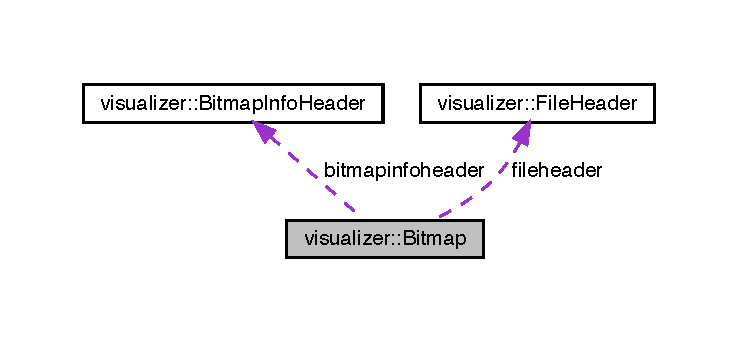
\includegraphics[width=350pt]{structvisualizer_1_1_bitmap__coll__graph}
\end{center}
\end{figure}
\subsection*{Public Attributes}
\begin{DoxyCompactItemize}
\item 
\mbox{\Hypertarget{structvisualizer_1_1_bitmap_a35cd50ab96ca92a2f3cc92fbec0ccef0}\label{structvisualizer_1_1_bitmap_a35cd50ab96ca92a2f3cc92fbec0ccef0}} 
\mbox{\hyperlink{structvisualizer_1_1_file_header}{File\+Header}} {\bfseries fileheader}
\item 
\mbox{\Hypertarget{structvisualizer_1_1_bitmap_ae321d14404bf8daff08333b6b2858603}\label{structvisualizer_1_1_bitmap_ae321d14404bf8daff08333b6b2858603}} 
\mbox{\hyperlink{structvisualizer_1_1_bitmap_info_header}{Bitmap\+Info\+Header}} {\bfseries bitmapinfoheader}
\end{DoxyCompactItemize}


The documentation for this struct was generated from the following file\+:\begin{DoxyCompactItemize}
\item 
/\+Users/fjp/git/bachelor/visualizer/visualizer.\+cpp\end{DoxyCompactItemize}

\hypertarget{structvisualizer_1_1_bitmap_info_header}{}\section{visualizer\+:\+:Bitmap\+Info\+Header Struct Reference}
\label{structvisualizer_1_1_bitmap_info_header}\index{visualizer\+::\+Bitmap\+Info\+Header@{visualizer\+::\+Bitmap\+Info\+Header}}
\subsection*{Public Attributes}
\begin{DoxyCompactItemize}
\item 
\mbox{\Hypertarget{structvisualizer_1_1_bitmap_info_header_aa948614dcf785eb73fc5f8e6d167cffe}\label{structvisualizer_1_1_bitmap_info_header_aa948614dcf785eb73fc5f8e6d167cffe}} 
uint32\+\_\+t {\bfseries dibheadersize}
\item 
\mbox{\Hypertarget{structvisualizer_1_1_bitmap_info_header_adbdbe8eb51d35287f34011bb807e2cc9}\label{structvisualizer_1_1_bitmap_info_header_adbdbe8eb51d35287f34011bb807e2cc9}} 
uint32\+\_\+t {\bfseries width}
\item 
\mbox{\Hypertarget{structvisualizer_1_1_bitmap_info_header_a690035c63f73bca8e8f7dec8c34e57eb}\label{structvisualizer_1_1_bitmap_info_header_a690035c63f73bca8e8f7dec8c34e57eb}} 
uint32\+\_\+t {\bfseries height}
\item 
\mbox{\Hypertarget{structvisualizer_1_1_bitmap_info_header_a388f28427be89d01501baf6684334279}\label{structvisualizer_1_1_bitmap_info_header_a388f28427be89d01501baf6684334279}} 
uint16\+\_\+t {\bfseries planes}
\item 
\mbox{\Hypertarget{structvisualizer_1_1_bitmap_info_header_aae99ff5c9e392f5b9071e71e96214037}\label{structvisualizer_1_1_bitmap_info_header_aae99ff5c9e392f5b9071e71e96214037}} 
uint16\+\_\+t {\bfseries bitsperpixel}
\item 
\mbox{\Hypertarget{structvisualizer_1_1_bitmap_info_header_a96381aa9deebf9a89a47ccf84e686b17}\label{structvisualizer_1_1_bitmap_info_header_a96381aa9deebf9a89a47ccf84e686b17}} 
uint32\+\_\+t {\bfseries compression}
\item 
\mbox{\Hypertarget{structvisualizer_1_1_bitmap_info_header_a5f8c0e9eae60a612efb52b33cd52e3e1}\label{structvisualizer_1_1_bitmap_info_header_a5f8c0e9eae60a612efb52b33cd52e3e1}} 
uint32\+\_\+t {\bfseries imagesize}
\item 
\mbox{\Hypertarget{structvisualizer_1_1_bitmap_info_header_a5cc22a4fff1707a47ae60b2ac1f6be53}\label{structvisualizer_1_1_bitmap_info_header_a5cc22a4fff1707a47ae60b2ac1f6be53}} 
uint32\+\_\+t {\bfseries ypixelpermeter}
\item 
\mbox{\Hypertarget{structvisualizer_1_1_bitmap_info_header_a55f795ae6a8f855cbc3a9cad8d69b091}\label{structvisualizer_1_1_bitmap_info_header_a55f795ae6a8f855cbc3a9cad8d69b091}} 
uint32\+\_\+t {\bfseries xpixelpermeter}
\item 
\mbox{\Hypertarget{structvisualizer_1_1_bitmap_info_header_a828bf1dbc3f160913e1a835ad007056b}\label{structvisualizer_1_1_bitmap_info_header_a828bf1dbc3f160913e1a835ad007056b}} 
uint32\+\_\+t {\bfseries numcolorspallette}
\item 
\mbox{\Hypertarget{structvisualizer_1_1_bitmap_info_header_a3569cfb8679eec61adfa907348e5c898}\label{structvisualizer_1_1_bitmap_info_header_a3569cfb8679eec61adfa907348e5c898}} 
uint32\+\_\+t {\bfseries mostimpcolor}
\end{DoxyCompactItemize}


The documentation for this struct was generated from the following file\+:\begin{DoxyCompactItemize}
\item 
/\+Users/fjp/git/bachelor/bachelor-\/master\+\_\+updated\+\_\+vfinal/visualizer/visualizer.\+cpp\end{DoxyCompactItemize}

\hypertarget{classplanner_1_1c_audi_rover}{}\section{planner\+:\+:c\+Audi\+Rover Class Reference}
\label{classplanner_1_1c_audi_rover}\index{planner\+::c\+Audi\+Rover@{planner\+::c\+Audi\+Rover}}
Inheritance diagram for planner\+:\+:c\+Audi\+Rover\+:\begin{figure}[H]
\begin{center}
\leavevmode
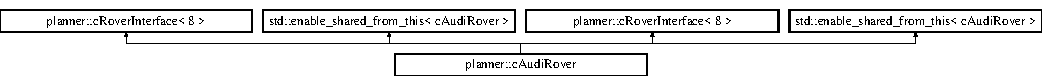
\includegraphics[height=2.000000cm]{classplanner_1_1c_audi_rover}
\end{center}
\end{figure}
\subsection*{Public Member Functions}
\begin{DoxyCompactItemize}
\item 
\mbox{\hyperlink{classplanner_1_1c_audi_rover_a433acb819672e065324dbbdb2a077ecb}{c\+Audi\+Rover}} (uint8\+\_\+t $\ast$i\+\_\+po\+Elevation, uint8\+\_\+t $\ast$i\+\_\+po\+Overrides, uint32\+\_\+t i\+\_\+n\+Height, uint32\+\_\+t i\+\_\+n\+Width)
\item 
\mbox{\Hypertarget{classplanner_1_1c_audi_rover_a52c48afa0829f858c19d3ecf4940db21}\label{classplanner_1_1c_audi_rover_a52c48afa0829f858c19d3ecf4940db21}} 
void \mbox{\hyperlink{classplanner_1_1c_audi_rover_a52c48afa0829f858c19d3ecf4940db21}{Summon}} (uint8\+\_\+t i\+\_\+n\+Step\+Size=1, uint8\+\_\+t i\+\_\+n\+Velocity=1)
\begin{DoxyCompactList}\small\item\em The summon feature that the Audi rover provides. \end{DoxyCompactList}\item 
\mbox{\Hypertarget{classplanner_1_1c_audi_rover_a7a463160a532a99e06a98fce3df4d2c3}\label{classplanner_1_1c_audi_rover_a7a463160a532a99e06a98fce3df4d2c3}} 
void {\bfseries Initialize\+Planner} (const uint8\+\_\+t \&i\+\_\+n\+Step\+Size, const uint8\+\_\+t \&i\+\_\+n\+Velocity) override
\end{DoxyCompactItemize}
\subsection*{Additional Inherited Members}


\subsection{Constructor \& Destructor Documentation}
\mbox{\Hypertarget{classplanner_1_1c_audi_rover_a433acb819672e065324dbbdb2a077ecb}\label{classplanner_1_1c_audi_rover_a433acb819672e065324dbbdb2a077ecb}} 
\index{planner\+::c\+Audi\+Rover@{planner\+::c\+Audi\+Rover}!c\+Audi\+Rover@{c\+Audi\+Rover}}
\index{c\+Audi\+Rover@{c\+Audi\+Rover}!planner\+::c\+Audi\+Rover@{planner\+::c\+Audi\+Rover}}
\subsubsection{\texorpdfstring{c\+Audi\+Rover()}{cAudiRover()}}
{\footnotesize\ttfamily planner\+::c\+Audi\+Rover\+::c\+Audi\+Rover (\begin{DoxyParamCaption}\item[{uint8\+\_\+t $\ast$}]{i\+\_\+po\+Elevation,  }\item[{uint8\+\_\+t $\ast$}]{i\+\_\+po\+Overrides,  }\item[{uint32\+\_\+t}]{i\+\_\+n\+Height,  }\item[{uint32\+\_\+t}]{i\+\_\+n\+Width }\end{DoxyParamCaption})}

Define direction and cost of different possible actions 

The documentation for this class was generated from the following files\+:\begin{DoxyCompactItemize}
\item 
/\+Users/fjp/git/bachelor/planner/include/audi\+\_\+rover.\+h\item 
/\+Users/fjp/git/bachelor/planner/src/audi\+\_\+rover.\+cpp\end{DoxyCompactItemize}

\hypertarget{classplanner_1_1c_graph}{}\section{planner\+:\+:c\+Graph Class Reference}
\label{classplanner_1_1c_graph}\index{planner\+::c\+Graph@{planner\+::c\+Graph}}


The map class c\+Map has pointers to the elevation.\+data (m\+\_\+po\+Elevation) and overrides.\+data (m\+\_\+po\+Overrides).  




{\ttfamily \#include $<$graph.\+h$>$}

\subsection*{Public Member Functions}
\begin{DoxyCompactItemize}
\item 
\mbox{\Hypertarget{classplanner_1_1c_graph_a189aeb64fe91fd6dd07f4b068d3b791e}\label{classplanner_1_1c_graph_a189aeb64fe91fd6dd07f4b068d3b791e}} 
\mbox{\hyperlink{classplanner_1_1c_graph_a189aeb64fe91fd6dd07f4b068d3b791e}{c\+Graph}} (uint8\+\_\+t $\ast$i\+\_\+o\+Elevation, uint8\+\_\+t $\ast$i\+\_\+o\+Overrides, int i\+\_\+n\+Height, int i\+\_\+n\+Width)
\begin{DoxyCompactList}\small\item\em Initializes the members m\+\_\+po\+Elevation, m\+\_\+po\+Overrides and the maps height m\+\_\+n\+Height and width m\+\_\+n\+Width. \end{DoxyCompactList}\item 
uint8\+\_\+t \mbox{\hyperlink{classplanner_1_1c_graph_a0e01eaa240f5e4f5020df2d611ab1994}{Elevation}} (int i\+\_\+nX, int i\+\_\+nY)
\begin{DoxyCompactList}\small\item\em Get elevation at provided location. \end{DoxyCompactList}\item 
\mbox{\Hypertarget{classplanner_1_1c_graph_adf0a3350d15819b92ec14c4596ebf702}\label{classplanner_1_1c_graph_adf0a3350d15819b92ec14c4596ebf702}} 
uint8\+\_\+t {\bfseries Overrides} (int i\+\_\+nX, int i\+\_\+nY)
\item 
bool \mbox{\hyperlink{classplanner_1_1c_graph_a97108b0e05fa547c006d76e749d52f27}{Water}} (int i\+\_\+nX, int i\+\_\+nY)
\begin{DoxyCompactList}\small\item\em Check if the position is on mainland or water. \end{DoxyCompactList}\item 
bool \mbox{\hyperlink{classplanner_1_1c_graph_a99935ff4c32d229e6006aaa843a685a9}{Water}} (int i\+\_\+n\+X0, int i\+\_\+n\+Y0, int i\+\_\+n\+X1, int i\+\_\+n\+Y1)
\begin{DoxyCompactList}\small\item\em Check if the position between the two locations is on mainland or water or goes through it. \end{DoxyCompactList}\item 
int \mbox{\hyperlink{classplanner_1_1c_graph_a5c163af76e19303794a908304f3b759e}{Height}} () const
\begin{DoxyCompactList}\small\item\em Getter for the height of the map, stored in m\+\_\+n\+Height. \end{DoxyCompactList}\item 
int \mbox{\hyperlink{classplanner_1_1c_graph_a25e3f4ee33c86a8a0c3a31c42dac7607}{Width}} () const
\begin{DoxyCompactList}\small\item\em Getter for the width of the map, stored in m\+\_\+n\+Width. \end{DoxyCompactList}\item 
void \mbox{\hyperlink{classplanner_1_1c_graph_a6da6e6e269013628aef48245a7787cb9}{Set\+Overrides}} (int i\+\_\+nX, int i\+\_\+nY, uint8\+\_\+t i\+\_\+n\+Value)
\begin{DoxyCompactList}\small\item\em Sets the provided overrides m\+\_\+po\+Overrides 8 bit value i\+\_\+n\+Value at the provided location while keeping the old value (or operation). \end{DoxyCompactList}\end{DoxyCompactItemize}
\subsection*{Public Attributes}
\begin{DoxyCompactItemize}
\item 
\mbox{\Hypertarget{classplanner_1_1c_graph_aea1ab1d83e0e58f454f07a46fc0d40dd}\label{classplanner_1_1c_graph_aea1ab1d83e0e58f454f07a46fc0d40dd}} 
uint8\+\_\+t $\ast$ \mbox{\hyperlink{classplanner_1_1c_graph_aea1ab1d83e0e58f454f07a46fc0d40dd}{m\+\_\+o\+Elevation}}
\begin{DoxyCompactList}\small\item\em Elevation over the ground (0-\/255). \end{DoxyCompactList}\item 
\mbox{\Hypertarget{classplanner_1_1c_graph_a0794d9865c56cddd3d051e6ea0c1c756}\label{classplanner_1_1c_graph_a0794d9865c56cddd3d051e6ea0c1c756}} 
uint8\+\_\+t $\ast$ {\bfseries m\+\_\+o\+Overrides}
\item 
\mbox{\Hypertarget{classplanner_1_1c_graph_a5bb5ea1aa1709b4530bbf5f931c1f277}\label{classplanner_1_1c_graph_a5bb5ea1aa1709b4530bbf5f931c1f277}} 
int \mbox{\hyperlink{classplanner_1_1c_graph_a5bb5ea1aa1709b4530bbf5f931c1f277}{m\+\_\+n\+Height}}
\begin{DoxyCompactList}\small\item\em Stores the height of the map. \end{DoxyCompactList}\item 
\mbox{\Hypertarget{classplanner_1_1c_graph_a91f89c2fde0344dc74060297b2d5235e}\label{classplanner_1_1c_graph_a91f89c2fde0344dc74060297b2d5235e}} 
int \mbox{\hyperlink{classplanner_1_1c_graph_a91f89c2fde0344dc74060297b2d5235e}{m\+\_\+n\+Width}}
\begin{DoxyCompactList}\small\item\em Stores the width of the map. \end{DoxyCompactList}\end{DoxyCompactItemize}


\subsection{Detailed Description}
The map class c\+Map has pointers to the elevation.\+data (m\+\_\+po\+Elevation) and overrides.\+data (m\+\_\+po\+Overrides). 

This class is used to check for constraints in the map (e.\+g. water basins, rivers and marsh, which cannot be traversed by the robot. The elevation data is used to model the acceleration of the rover. 

\subsection{Member Function Documentation}
\mbox{\Hypertarget{classplanner_1_1c_graph_a0e01eaa240f5e4f5020df2d611ab1994}\label{classplanner_1_1c_graph_a0e01eaa240f5e4f5020df2d611ab1994}} 
\index{planner\+::c\+Graph@{planner\+::c\+Graph}!Elevation@{Elevation}}
\index{Elevation@{Elevation}!planner\+::c\+Graph@{planner\+::c\+Graph}}
\subsubsection{\texorpdfstring{Elevation()}{Elevation()}}
{\footnotesize\ttfamily uint8\+\_\+t planner\+::c\+Graph\+::\+Elevation (\begin{DoxyParamCaption}\item[{int}]{i\+\_\+nX,  }\item[{int}]{i\+\_\+nY }\end{DoxyParamCaption})}



Get elevation at provided location. 

From the read elevation.\+data the 8 bit value is returned. 
\begin{DoxyParams}[1]{Parameters}
\mbox{\tt in}  & {\em i\+\_\+nX} & X location of the elevation. \\
\hline
\mbox{\tt in}  & {\em i\+\_\+nY} & Y location of the elevation. \\
\hline
\end{DoxyParams}
\begin{DoxyReturn}{Returns}
Elevation at (i\+\_\+nX, i\+\_\+nY). 
\end{DoxyReturn}
\mbox{\Hypertarget{classplanner_1_1c_graph_a5c163af76e19303794a908304f3b759e}\label{classplanner_1_1c_graph_a5c163af76e19303794a908304f3b759e}} 
\index{planner\+::c\+Graph@{planner\+::c\+Graph}!Height@{Height}}
\index{Height@{Height}!planner\+::c\+Graph@{planner\+::c\+Graph}}
\subsubsection{\texorpdfstring{Height()}{Height()}}
{\footnotesize\ttfamily int planner\+::c\+Graph\+::\+Height (\begin{DoxyParamCaption}{ }\end{DoxyParamCaption}) const}



Getter for the height of the map, stored in m\+\_\+n\+Height. 

\begin{DoxyReturn}{Returns}
The total height of the map. 
\end{DoxyReturn}
\mbox{\Hypertarget{classplanner_1_1c_graph_a6da6e6e269013628aef48245a7787cb9}\label{classplanner_1_1c_graph_a6da6e6e269013628aef48245a7787cb9}} 
\index{planner\+::c\+Graph@{planner\+::c\+Graph}!Set\+Overrides@{Set\+Overrides}}
\index{Set\+Overrides@{Set\+Overrides}!planner\+::c\+Graph@{planner\+::c\+Graph}}
\subsubsection{\texorpdfstring{Set\+Overrides()}{SetOverrides()}}
{\footnotesize\ttfamily void planner\+::c\+Graph\+::\+Set\+Overrides (\begin{DoxyParamCaption}\item[{int}]{i\+\_\+nX,  }\item[{int}]{i\+\_\+nY,  }\item[{uint8\+\_\+t}]{i\+\_\+n\+Value }\end{DoxyParamCaption})}



Sets the provided overrides m\+\_\+po\+Overrides 8 bit value i\+\_\+n\+Value at the provided location while keeping the old value (or operation). 


\begin{DoxyParams}[1]{Parameters}
\mbox{\tt in}  & {\em i\+\_\+nX} & X location of the overrides m\+\_\+po\+Overrides that should be updated. \\
\hline
\mbox{\tt in}  & {\em i\+\_\+nY} & Y location of the overrides m\+\_\+po\+Overrides that should be updated. \\
\hline
\mbox{\tt in}  & {\em i\+\_\+n\+Value} & The or operator is applied to this 8 bit mask value and the current overrides value at (i\+\_\+nX, i\+\_\+nY). \\
\hline
\end{DoxyParams}
\mbox{\Hypertarget{classplanner_1_1c_graph_a97108b0e05fa547c006d76e749d52f27}\label{classplanner_1_1c_graph_a97108b0e05fa547c006d76e749d52f27}} 
\index{planner\+::c\+Graph@{planner\+::c\+Graph}!Water@{Water}}
\index{Water@{Water}!planner\+::c\+Graph@{planner\+::c\+Graph}}
\subsubsection{\texorpdfstring{Water()}{Water()}\hspace{0.1cm}{\footnotesize\ttfamily [1/2]}}
{\footnotesize\ttfamily bool planner\+::c\+Graph\+::\+Water (\begin{DoxyParamCaption}\item[{int}]{i\+\_\+nX,  }\item[{int}]{i\+\_\+nY }\end{DoxyParamCaption})}



Check if the position is on mainland or water. 


\begin{DoxyParams}[1]{Parameters}
\mbox{\tt in}  & {\em i\+\_\+nX} & X coordinate to be checked for water. \\
\hline
\mbox{\tt in}  & {\em i\+\_\+nY} & Y coordinate to be checked for water. \\
\hline
\end{DoxyParams}
\begin{DoxyReturn}{Returns}
true if the provided position is on water, false otherwise. 
\end{DoxyReturn}
\mbox{\Hypertarget{classplanner_1_1c_graph_a99935ff4c32d229e6006aaa843a685a9}\label{classplanner_1_1c_graph_a99935ff4c32d229e6006aaa843a685a9}} 
\index{planner\+::c\+Graph@{planner\+::c\+Graph}!Water@{Water}}
\index{Water@{Water}!planner\+::c\+Graph@{planner\+::c\+Graph}}
\subsubsection{\texorpdfstring{Water()}{Water()}\hspace{0.1cm}{\footnotesize\ttfamily [2/2]}}
{\footnotesize\ttfamily bool planner\+::c\+Graph\+::\+Water (\begin{DoxyParamCaption}\item[{int}]{i\+\_\+n\+X0,  }\item[{int}]{i\+\_\+n\+Y0,  }\item[{int}]{i\+\_\+n\+X1,  }\item[{int}]{i\+\_\+n\+Y1 }\end{DoxyParamCaption})}



Check if the position between the two locations is on mainland or water or goes through it. 


\begin{DoxyParams}[1]{Parameters}
\mbox{\tt in}  & {\em i\+\_\+nX} & X coordinate to be checked for water. \\
\hline
\mbox{\tt in}  & {\em i\+\_\+nY} & Y coordinate to be checked for water. \\
\hline
\end{DoxyParams}
\begin{DoxyReturn}{Returns}
true if the provided position is on or goes through water, false otherwise. 
\end{DoxyReturn}
\mbox{\Hypertarget{classplanner_1_1c_graph_a25e3f4ee33c86a8a0c3a31c42dac7607}\label{classplanner_1_1c_graph_a25e3f4ee33c86a8a0c3a31c42dac7607}} 
\index{planner\+::c\+Graph@{planner\+::c\+Graph}!Width@{Width}}
\index{Width@{Width}!planner\+::c\+Graph@{planner\+::c\+Graph}}
\subsubsection{\texorpdfstring{Width()}{Width()}}
{\footnotesize\ttfamily int planner\+::c\+Graph\+::\+Width (\begin{DoxyParamCaption}{ }\end{DoxyParamCaption}) const}



Getter for the width of the map, stored in m\+\_\+n\+Width. 

\begin{DoxyReturn}{Returns}
The total width of the map. 
\end{DoxyReturn}


The documentation for this class was generated from the following files\+:\begin{DoxyCompactItemize}
\item 
/\+Users/fjp/git/bachelor/planner/include/graph.\+h\item 
/\+Users/fjp/git/bachelor/planner/src/graph.\+cpp\end{DoxyCompactItemize}

\hypertarget{classplanner_1_1c_planner}{}\section{planner\+:\+:c\+Planner Class Reference}
\label{classplanner_1_1c_planner}\index{planner\+::c\+Planner@{planner\+::c\+Planner}}


Implements the planner interface c\+Planner\+Interface$<$size\+\_\+t Directions$>$ with an action vector of size eight.  




{\ttfamily \#include $<$planner.\+h$>$}

Inheritance diagram for planner\+:\+:c\+Planner\+:\begin{figure}[H]
\begin{center}
\leavevmode
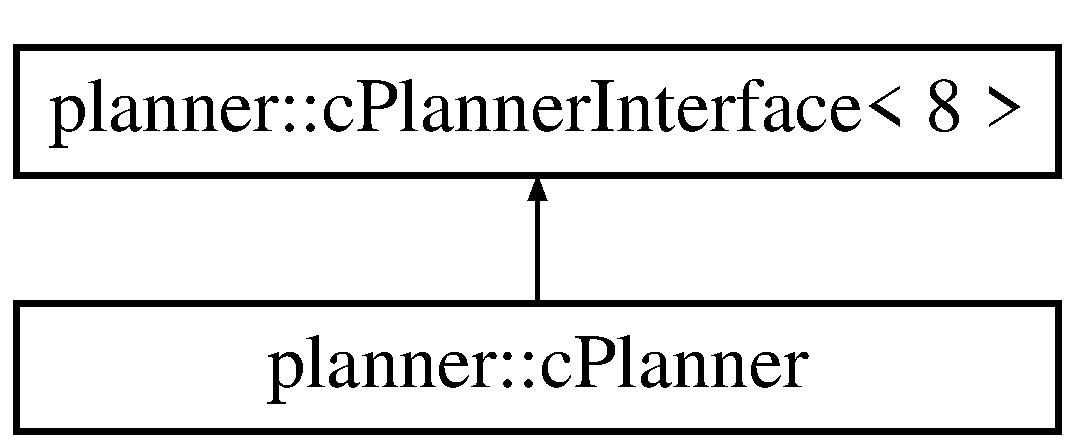
\includegraphics[height=2.000000cm]{classplanner_1_1c_planner}
\end{center}
\end{figure}
\subsection*{Public Types}
\begin{DoxyCompactItemize}
\item 
\mbox{\Hypertarget{classplanner_1_1c_planner_a7f6dc4cbb69dd1ede14a67b0a7bd425b}\label{classplanner_1_1c_planner_a7f6dc4cbb69dd1ede14a67b0a7bd425b}} 
enum \mbox{\hyperlink{classplanner_1_1c_planner_a7f6dc4cbb69dd1ede14a67b0a7bd425b}{t\+Heuristic}} \{ {\bfseries M\+A\+N\+H\+A\+T\+T\+EN}, 
{\bfseries E\+U\+C\+L\+I\+D\+E\+AN}, 
{\bfseries O\+C\+T\+I\+LE}, 
{\bfseries C\+H\+E\+B\+Y\+S\+H\+EV}
 \}
\begin{DoxyCompactList}\small\item\em Types of heuristics that can be calculated with \mbox{\hyperlink{classplanner_1_1c_planner_ad32a7c58b885456ced172b66fed854f0}{Update\+Heuristic()}} \end{DoxyCompactList}\end{DoxyCompactItemize}
\subsection*{Public Member Functions}
\begin{DoxyCompactItemize}
\item 
\mbox{\hyperlink{classplanner_1_1c_planner_a4f425d47b277f000d34df04de9995274}{c\+Planner}} (\mbox{\hyperlink{classplanner_1_1c_rover_interface}{c\+Rover\+Interface}}$<$ 8 $>$ $\ast$i\+\_\+po\+Rover, \mbox{\hyperlink{classplanner_1_1c_graph}{c\+Graph}} \&i\+\_\+o\+Map)
\begin{DoxyCompactList}\small\item\em Initializes member variables m\+\_\+po\+Rover and m\+\_\+o\+Map and calls Calculate\+Consistency\+Factor(). \end{DoxyCompactList}\item 
\mbox{\Hypertarget{classplanner_1_1c_planner_aa9ae1109d3c4b7ac19aef2616547654e}\label{classplanner_1_1c_planner_aa9ae1109d3c4b7ac19aef2616547654e}} 
\mbox{\hyperlink{classplanner_1_1c_planner_aa9ae1109d3c4b7ac19aef2616547654e}{$\sim$c\+Planner}} ()
\begin{DoxyCompactList}\small\item\em Destructor to delete the allocated memory. \end{DoxyCompactList}\item 
float \mbox{\hyperlink{classplanner_1_1c_planner_a7c4defd454429503d4e47b552a5311fb}{Plan}} () override
\begin{DoxyCompactList}\small\item\em Override of the base interface \mbox{\hyperlink{classplanner_1_1c_planner_interface}{c\+Planner\+Interface}}, which invokes the A\+Star() search algorithm. \end{DoxyCompactList}\item 
void \mbox{\hyperlink{classplanner_1_1c_planner_a1a4650050656545744796296a653d388}{Generate\+Heuristic}} ()
\begin{DoxyCompactList}\small\item\em Output distance heuristic map to file, which is used to generate the Matlab plot. \end{DoxyCompactList}\item 
float \mbox{\hyperlink{classplanner_1_1c_planner_ad32a7c58b885456ced172b66fed854f0}{Update\+Heuristic}} (\mbox{\hyperlink{structplanner_1_1t_node}{t\+Node}} $\ast$i\+\_\+s\+Node, const \mbox{\hyperlink{classplanner_1_1c_planner_a7f6dc4cbb69dd1ede14a67b0a7bd425b}{t\+Heuristic}} i\+\_\+e\+Heuristic=O\+C\+T\+I\+LE) const
\begin{DoxyCompactList}\small\item\em Updates the heuristic value of the node argument i\+\_\+s\+Node. \end{DoxyCompactList}\item 
float \mbox{\hyperlink{classplanner_1_1c_planner_a7d5f7f89a10b66f19c0257cbf7f2afbb}{Update\+Heuristic}} (const \mbox{\hyperlink{structplanner_1_1t_location}{t\+Location}} \&i\+\_\+s\+Location, const \mbox{\hyperlink{classplanner_1_1c_planner_a7f6dc4cbb69dd1ede14a67b0a7bd425b}{t\+Heuristic}} i\+\_\+e\+Heuristic=O\+C\+T\+I\+LE) const
\begin{DoxyCompactList}\small\item\em Updates the heuristic value of the node located at tlocation i\+\_\+s\+Location. \end{DoxyCompactList}\item 
void \mbox{\hyperlink{classplanner_1_1c_planner_a8b4f67bd192db4784c6ab95c11e51a16}{Heuristic\+Check}} (\mbox{\hyperlink{structplanner_1_1t_node}{t\+Node}} $\ast$i\+\_\+s\+Node) const
\begin{DoxyCompactList}\small\item\em Check if the heuristic of node i\+\_\+s\+Node is consistent. \end{DoxyCompactList}\item 
void \mbox{\hyperlink{classplanner_1_1c_planner_a82e45fc2701e90d3fa9df72f475e455e}{Update\+Cost}} (\mbox{\hyperlink{structplanner_1_1t_node}{t\+Node}} $\ast$i\+\_\+s\+Node) const
\begin{DoxyCompactList}\small\item\em Updates the node argument with its path cost $g(n)$ with island seconds as its unit. \end{DoxyCompactList}\item 
bool \mbox{\hyperlink{classplanner_1_1c_planner_ac5119e3243d9f6747f1da0ed6d356642}{Within\+Map}} (const \mbox{\hyperlink{structplanner_1_1t_location}{t\+Location}} \&i\+\_\+s\+Location) const
\begin{DoxyCompactList}\small\item\em Test if the provided location i\+\_\+s\+Location lies within the map. \end{DoxyCompactList}\item 
virtual bool \mbox{\hyperlink{classplanner_1_1c_planner_a8b241ebd7bb3bde3dd062c50a2a42339}{Goal\+Test}} (const \mbox{\hyperlink{structplanner_1_1t_node}{t\+Node}} $\ast$i\+\_\+s\+First, const \mbox{\hyperlink{structplanner_1_1t_node}{t\+Node}} $\ast$i\+\_\+s\+Second) const override
\begin{DoxyCompactList}\small\item\em Goal test to check if the two provided nodes i\+\_\+s\+First, i\+\_\+s\+Second are equal. \end{DoxyCompactList}\item 
\mbox{\hyperlink{structplanner_1_1t_node}{t\+Node}} $\ast$ \mbox{\hyperlink{classplanner_1_1c_planner_a7ddb18b161e5d59cfe733bce32c31896}{Child}} (\mbox{\hyperlink{structplanner_1_1t_node}{t\+Node}} $\ast$i\+\_\+s\+Parent, const \mbox{\hyperlink{structplanner_1_1t_action}{t\+Action}} \&i\+\_\+s\+Action) const override
\begin{DoxyCompactList}\small\item\em Generate a successor node state given a node i\+\_\+s\+Parent and action i\+\_\+s\+Action. \end{DoxyCompactList}\item 
bool \mbox{\hyperlink{classplanner_1_1c_planner_a34b0582ca32cc235837c0b638b39e3af}{Traversable}} (\mbox{\hyperlink{structplanner_1_1t_node}{t\+Node}} $\ast$i\+\_\+s\+Current, \mbox{\hyperlink{structplanner_1_1t_node}{t\+Node}} $\ast$i\+\_\+s\+Next) const
\begin{DoxyCompactList}\small\item\em considers step size of rover and checks if the path is traversable T\+O\+DO improve comment \end{DoxyCompactList}\item 
void \mbox{\hyperlink{classplanner_1_1c_planner_ad9389067cbc3fa6fb1c2efdf3f344664}{Traverse\+Path}} (\mbox{\hyperlink{structplanner_1_1t_node}{t\+Node}} $\ast$i\+\_\+ps\+Node) const override
\begin{DoxyCompactList}\small\item\em Given the node i\+\_\+ps\+Node the overrides map m\+\_\+po\+Overrides is updated for displaying the path. \end{DoxyCompactList}\item 
\mbox{\Hypertarget{classplanner_1_1c_planner_aa90d751ce544870e4c89494e06fdac6c}\label{classplanner_1_1c_planner_aa90d751ce544870e4c89494e06fdac6c}} 
const int \mbox{\hyperlink{classplanner_1_1c_planner_aa90d751ce544870e4c89494e06fdac6c}{GradX}} (int i\+\_\+nX, int i\+\_\+nY) const
\begin{DoxyCompactList}\small\item\em Calculates the discrete gradient of the map m\+\_\+po\+Map in x direction. \end{DoxyCompactList}\item 
\mbox{\Hypertarget{classplanner_1_1c_planner_a6fd8e8632d78d85ce472322267ba7b36}\label{classplanner_1_1c_planner_a6fd8e8632d78d85ce472322267ba7b36}} 
const int \mbox{\hyperlink{classplanner_1_1c_planner_a6fd8e8632d78d85ce472322267ba7b36}{GradY}} (int i\+\_\+nX, int i\+\_\+nY) const
\begin{DoxyCompactList}\small\item\em Calculates the discrete gradient of the map m\+\_\+po\+Map in y direction. \end{DoxyCompactList}\item 
uint32\+\_\+t \mbox{\hyperlink{classplanner_1_1c_planner_a5ae4464a4d418cda71f4a8133d592c93}{Node\+Hash}} (const \mbox{\hyperlink{structplanner_1_1t_node}{t\+Node}} $\ast$i\+\_\+s\+Node) const
\begin{DoxyCompactList}\small\item\em Calculates the node hash using its location and the width of the map. \end{DoxyCompactList}\end{DoxyCompactItemize}
\subsection*{Additional Inherited Members}


\subsection{Detailed Description}
Implements the planner interface c\+Planner\+Interface$<$size\+\_\+t Directions$>$ with an action vector of size eight. 

\subsection{Constructor \& Destructor Documentation}
\mbox{\Hypertarget{classplanner_1_1c_planner_a4f425d47b277f000d34df04de9995274}\label{classplanner_1_1c_planner_a4f425d47b277f000d34df04de9995274}} 
\index{planner\+::c\+Planner@{planner\+::c\+Planner}!c\+Planner@{c\+Planner}}
\index{c\+Planner@{c\+Planner}!planner\+::c\+Planner@{planner\+::c\+Planner}}
\subsubsection{\texorpdfstring{c\+Planner()}{cPlanner()}}
{\footnotesize\ttfamily planner\+::c\+Planner\+::c\+Planner (\begin{DoxyParamCaption}\item[{\mbox{\hyperlink{classplanner_1_1c_rover_interface}{c\+Rover\+Interface}}$<$ 8 $>$ $\ast$}]{i\+\_\+po\+Rover,  }\item[{\mbox{\hyperlink{classplanner_1_1c_graph}{c\+Graph}} \&}]{i\+\_\+o\+Map }\end{DoxyParamCaption})}



Initializes member variables m\+\_\+po\+Rover and m\+\_\+o\+Map and calls Calculate\+Consistency\+Factor(). 

The 

\subsection{Member Function Documentation}
\mbox{\Hypertarget{classplanner_1_1c_planner_a7ddb18b161e5d59cfe733bce32c31896}\label{classplanner_1_1c_planner_a7ddb18b161e5d59cfe733bce32c31896}} 
\index{planner\+::c\+Planner@{planner\+::c\+Planner}!Child@{Child}}
\index{Child@{Child}!planner\+::c\+Planner@{planner\+::c\+Planner}}
\subsubsection{\texorpdfstring{Child()}{Child()}}
{\footnotesize\ttfamily \mbox{\hyperlink{structplanner_1_1t_node}{t\+Node}} $\ast$ planner\+::c\+Planner\+::\+Child (\begin{DoxyParamCaption}\item[{\mbox{\hyperlink{structplanner_1_1t_node}{t\+Node}} $\ast$}]{i\+\_\+s\+Parent,  }\item[{const \mbox{\hyperlink{structplanner_1_1t_action}{t\+Action}} \&}]{i\+\_\+s\+Action }\end{DoxyParamCaption}) const\hspace{0.3cm}{\ttfamily [override]}, {\ttfamily [virtual]}}



Generate a successor node state given a node i\+\_\+s\+Parent and action i\+\_\+s\+Action. 

Overrides method of the base class inteface c\+Planner\+Interface$<$size\+\_\+t Directions$>$. Defines a new node on the heap and initializes it according to the given action.


\begin{DoxyParams}[1]{Parameters}
\mbox{\tt in}  & {\em i\+\_\+s\+Parent} & node which becomes the parent of the new node. \\
\hline
\mbox{\tt in}  & {\em i\+\_\+s\+Action} & struct of type \mbox{\hyperlink{structplanner_1_1t_action}{t\+Action}} that contains the direction and cost of the action. \\
\hline
\end{DoxyParams}
Calculate hash of node using its location 

Implements \mbox{\hyperlink{classplanner_1_1c_planner_interface_a499d8d3b81b0090318f4f2ea044c084c}{planner\+::c\+Planner\+Interface$<$ 8 $>$}}.

\mbox{\Hypertarget{classplanner_1_1c_planner_a1a4650050656545744796296a653d388}\label{classplanner_1_1c_planner_a1a4650050656545744796296a653d388}} 
\index{planner\+::c\+Planner@{planner\+::c\+Planner}!Generate\+Heuristic@{Generate\+Heuristic}}
\index{Generate\+Heuristic@{Generate\+Heuristic}!planner\+::c\+Planner@{planner\+::c\+Planner}}
\subsubsection{\texorpdfstring{Generate\+Heuristic()}{GenerateHeuristic()}}
{\footnotesize\ttfamily void planner\+::c\+Planner\+::\+Generate\+Heuristic (\begin{DoxyParamCaption}{ }\end{DoxyParamCaption})}



Output distance heuristic map to file, which is used to generate the Matlab plot. 

This implementation calls \mbox{\hyperlink{classplanner_1_1c_planner_ad32a7c58b885456ced172b66fed854f0}{Update\+Heuristic()}} to calculate a distance heuristic. Because the robot can move in eight directions the octile distance heuristic is calculated. Other possible gird map heuristics are Manhatten, Chebyshev and Euclidean. Output octile distance \mbox{\Hypertarget{classplanner_1_1c_planner_a8b241ebd7bb3bde3dd062c50a2a42339}\label{classplanner_1_1c_planner_a8b241ebd7bb3bde3dd062c50a2a42339}} 
\index{planner\+::c\+Planner@{planner\+::c\+Planner}!Goal\+Test@{Goal\+Test}}
\index{Goal\+Test@{Goal\+Test}!planner\+::c\+Planner@{planner\+::c\+Planner}}
\subsubsection{\texorpdfstring{Goal\+Test()}{GoalTest()}}
{\footnotesize\ttfamily bool planner\+::c\+Planner\+::\+Goal\+Test (\begin{DoxyParamCaption}\item[{const \mbox{\hyperlink{structplanner_1_1t_node}{t\+Node}} $\ast$}]{i\+\_\+s\+First,  }\item[{const \mbox{\hyperlink{structplanner_1_1t_node}{t\+Node}} $\ast$}]{i\+\_\+s\+Second }\end{DoxyParamCaption}) const\hspace{0.3cm}{\ttfamily [override]}, {\ttfamily [virtual]}}



Goal test to check if the two provided nodes i\+\_\+s\+First, i\+\_\+s\+Second are equal. 

Note that this check takes the step size m\+\_\+n\+Step\+Size of the rover into account. This allows to set a step size greater than one, which can be used for debugging. 
\begin{DoxyParams}[1]{Parameters}
\mbox{\tt in}  & {\em i\+\_\+s\+First} & could be the current node that needs to be checked. \\
\hline
\mbox{\tt in}  & {\em i\+\_\+s\+Second} & could be the goal node. \\
\hline
\end{DoxyParams}
\begin{DoxyReturn}{Returns}
true or false if the two nodes are equal. 
\end{DoxyReturn}


Implements \mbox{\hyperlink{classplanner_1_1c_planner_interface_aadc6ccb9088f755bd0ec30046bb79e99}{planner\+::c\+Planner\+Interface$<$ 8 $>$}}.

\mbox{\Hypertarget{classplanner_1_1c_planner_a8b4f67bd192db4784c6ab95c11e51a16}\label{classplanner_1_1c_planner_a8b4f67bd192db4784c6ab95c11e51a16}} 
\index{planner\+::c\+Planner@{planner\+::c\+Planner}!Heuristic\+Check@{Heuristic\+Check}}
\index{Heuristic\+Check@{Heuristic\+Check}!planner\+::c\+Planner@{planner\+::c\+Planner}}
\subsubsection{\texorpdfstring{Heuristic\+Check()}{HeuristicCheck()}}
{\footnotesize\ttfamily void planner\+::c\+Planner\+::\+Heuristic\+Check (\begin{DoxyParamCaption}\item[{\mbox{\hyperlink{structplanner_1_1t_node}{t\+Node}} $\ast$}]{i\+\_\+s\+Node }\end{DoxyParamCaption}) const}



Check if the heuristic of node i\+\_\+s\+Node is consistent. 

Consistency is given if h(n) $<$= c(n,p) + h(p), where h(p) is the heuristic of the parent node and c(n,p) are the step costs from parent p to node n. 
\begin{DoxyParams}[1]{Parameters}
\mbox{\tt in}  & {\em i\+\_\+s\+Node} & the node which heuristic value is tested. \\
\hline
\end{DoxyParams}
\mbox{\Hypertarget{classplanner_1_1c_planner_a5ae4464a4d418cda71f4a8133d592c93}\label{classplanner_1_1c_planner_a5ae4464a4d418cda71f4a8133d592c93}} 
\index{planner\+::c\+Planner@{planner\+::c\+Planner}!Node\+Hash@{Node\+Hash}}
\index{Node\+Hash@{Node\+Hash}!planner\+::c\+Planner@{planner\+::c\+Planner}}
\subsubsection{\texorpdfstring{Node\+Hash()}{NodeHash()}}
{\footnotesize\ttfamily uint32\+\_\+t planner\+::c\+Planner\+::\+Node\+Hash (\begin{DoxyParamCaption}\item[{const \mbox{\hyperlink{structplanner_1_1t_node}{t\+Node}} $\ast$}]{i\+\_\+s\+Node }\end{DoxyParamCaption}) const}



Calculates the node hash using its location and the width of the map. 

The hash is required to sort the std\+::map$<$t\+Node$>$ o\+Cost of reaching a node, which is used in the A\+Star() search algorithm. \mbox{\Hypertarget{classplanner_1_1c_planner_a7c4defd454429503d4e47b552a5311fb}\label{classplanner_1_1c_planner_a7c4defd454429503d4e47b552a5311fb}} 
\index{planner\+::c\+Planner@{planner\+::c\+Planner}!Plan@{Plan}}
\index{Plan@{Plan}!planner\+::c\+Planner@{planner\+::c\+Planner}}
\subsubsection{\texorpdfstring{Plan()}{Plan()}}
{\footnotesize\ttfamily float planner\+::c\+Planner\+::\+Plan (\begin{DoxyParamCaption}{ }\end{DoxyParamCaption})\hspace{0.3cm}{\ttfamily [override]}, {\ttfamily [virtual]}}



Override of the base interface \mbox{\hyperlink{classplanner_1_1c_planner_interface}{c\+Planner\+Interface}}, which invokes the A\+Star() search algorithm. 

\begin{DoxyReturn}{Returns}
the time to travel from start to goal if it was found. Otherwise -\/1 is returned. 
\end{DoxyReturn}


Implements \mbox{\hyperlink{classplanner_1_1c_planner_interface_a4d8effce5ee5d097a30465280e9416d6}{planner\+::c\+Planner\+Interface$<$ 8 $>$}}.

\mbox{\Hypertarget{classplanner_1_1c_planner_a34b0582ca32cc235837c0b638b39e3af}\label{classplanner_1_1c_planner_a34b0582ca32cc235837c0b638b39e3af}} 
\index{planner\+::c\+Planner@{planner\+::c\+Planner}!Traversable@{Traversable}}
\index{Traversable@{Traversable}!planner\+::c\+Planner@{planner\+::c\+Planner}}
\subsubsection{\texorpdfstring{Traversable()}{Traversable()}}
{\footnotesize\ttfamily bool planner\+::c\+Planner\+::\+Traversable (\begin{DoxyParamCaption}\item[{\mbox{\hyperlink{structplanner_1_1t_node}{t\+Node}} $\ast$}]{i\+\_\+s\+Current,  }\item[{\mbox{\hyperlink{structplanner_1_1t_node}{t\+Node}} $\ast$}]{i\+\_\+s\+Next }\end{DoxyParamCaption}) const}



considers step size of rover and checks if the path is traversable T\+O\+DO improve comment 

Check if the intermediate locations moving from current node to next are on mainland or water

Next location lies outside the map \mbox{\Hypertarget{classplanner_1_1c_planner_ad9389067cbc3fa6fb1c2efdf3f344664}\label{classplanner_1_1c_planner_ad9389067cbc3fa6fb1c2efdf3f344664}} 
\index{planner\+::c\+Planner@{planner\+::c\+Planner}!Traverse\+Path@{Traverse\+Path}}
\index{Traverse\+Path@{Traverse\+Path}!planner\+::c\+Planner@{planner\+::c\+Planner}}
\subsubsection{\texorpdfstring{Traverse\+Path()}{TraversePath()}}
{\footnotesize\ttfamily void planner\+::c\+Planner\+::\+Traverse\+Path (\begin{DoxyParamCaption}\item[{\mbox{\hyperlink{structplanner_1_1t_node}{t\+Node}} $\ast$}]{i\+\_\+ps\+Node }\end{DoxyParamCaption}) const\hspace{0.3cm}{\ttfamily [override]}, {\ttfamily [virtual]}}



Given the node i\+\_\+ps\+Node the overrides map m\+\_\+po\+Overrides is updated for displaying the path. 

Traversing a path takes place using the m\+\_\+ps\+Parent field of the \mbox{\hyperlink{structplanner_1_1t_node}{t\+Node}} struct. 
\begin{DoxyParams}[1]{Parameters}
\mbox{\tt in}  & {\em i\+\_\+ps\+Node} & Goal node or any other which is traversed back \\
\hline
\end{DoxyParams}
Check if the current node is the start node, which has no parent and is therefore set to N\+U\+LL

Store path in overrides

Move towards the start 

Implements \mbox{\hyperlink{classplanner_1_1c_planner_interface_a5c30b547b681b04434102fbcc7c72ea3}{planner\+::c\+Planner\+Interface$<$ 8 $>$}}.

\mbox{\Hypertarget{classplanner_1_1c_planner_a82e45fc2701e90d3fa9df72f475e455e}\label{classplanner_1_1c_planner_a82e45fc2701e90d3fa9df72f475e455e}} 
\index{planner\+::c\+Planner@{planner\+::c\+Planner}!Update\+Cost@{Update\+Cost}}
\index{Update\+Cost@{Update\+Cost}!planner\+::c\+Planner@{planner\+::c\+Planner}}
\subsubsection{\texorpdfstring{Update\+Cost()}{UpdateCost()}}
{\footnotesize\ttfamily void planner\+::c\+Planner\+::\+Update\+Cost (\begin{DoxyParamCaption}\item[{\mbox{\hyperlink{structplanner_1_1t_node}{t\+Node}} $\ast$}]{i\+\_\+s\+Node }\end{DoxyParamCaption}) const}



Updates the node argument with its path cost $g(n)$ with island seconds as its unit. 

Uses the slope found from the gradient of the elevation map c\+Map\+::m\+\_\+o\+Elevation to calculate an acceleration value, where only its component in the x,y plane is used. The value is added to the time it takes for a straight or diagonal step (depending on the action of the node). The sum is stored in $g(n)$ of the node \mbox{\hyperlink{structplanner_1_1t_node}{planner\+::t\+Node}} i\+\_\+s\+Node. 
\begin{DoxyParams}[1]{Parameters}
\mbox{\tt in}  & {\em i\+\_\+s\+Node} & The node which path cost is updated. \\
\hline
\end{DoxyParams}
Rover\textquotesingle{}s normal speed is 1 cell per island second

Add action (step) cost, which is given in island seconds

If the rover is going up or down hill, calculate the acceleration on the inclined plane Calculate current gradient in step direction ~\newline
 Down hill \mbox{\Hypertarget{classplanner_1_1c_planner_ad32a7c58b885456ced172b66fed854f0}\label{classplanner_1_1c_planner_ad32a7c58b885456ced172b66fed854f0}} 
\index{planner\+::c\+Planner@{planner\+::c\+Planner}!Update\+Heuristic@{Update\+Heuristic}}
\index{Update\+Heuristic@{Update\+Heuristic}!planner\+::c\+Planner@{planner\+::c\+Planner}}
\subsubsection{\texorpdfstring{Update\+Heuristic()}{UpdateHeuristic()}\hspace{0.1cm}{\footnotesize\ttfamily [1/2]}}
{\footnotesize\ttfamily float planner\+::c\+Planner\+::\+Update\+Heuristic (\begin{DoxyParamCaption}\item[{\mbox{\hyperlink{structplanner_1_1t_node}{t\+Node}} $\ast$}]{i\+\_\+s\+Node,  }\item[{const \mbox{\hyperlink{classplanner_1_1c_planner_a7f6dc4cbb69dd1ede14a67b0a7bd425b}{t\+Heuristic}}}]{i\+\_\+e\+Heuristic = {\ttfamily OCTILE} }\end{DoxyParamCaption}) const}



Updates the heuristic value of the node argument i\+\_\+s\+Node. 

Calcualtes a grid map distance heuristic. Can be one of the heuristics defined in t\+Heuristic. 
\begin{DoxyParams}[1]{Parameters}
\mbox{\tt in}  & {\em i\+\_\+s\+Node} & the node which heuristic is updated \\
\hline
\mbox{\tt in}  & {\em i\+\_\+e\+Heuristic} & the type of heuristic to calculate, see t\+Heuristic. \\
\hline
\end{DoxyParams}
\begin{DoxyReturn}{Returns}
The calculated heuristic value. 
\end{DoxyReturn}
Correct heuristic value to get a consistent heuristic. Required because of moving up or down the hill. \mbox{\Hypertarget{classplanner_1_1c_planner_a7d5f7f89a10b66f19c0257cbf7f2afbb}\label{classplanner_1_1c_planner_a7d5f7f89a10b66f19c0257cbf7f2afbb}} 
\index{planner\+::c\+Planner@{planner\+::c\+Planner}!Update\+Heuristic@{Update\+Heuristic}}
\index{Update\+Heuristic@{Update\+Heuristic}!planner\+::c\+Planner@{planner\+::c\+Planner}}
\subsubsection{\texorpdfstring{Update\+Heuristic()}{UpdateHeuristic()}\hspace{0.1cm}{\footnotesize\ttfamily [2/2]}}
{\footnotesize\ttfamily float planner\+::c\+Planner\+::\+Update\+Heuristic (\begin{DoxyParamCaption}\item[{const \mbox{\hyperlink{structplanner_1_1t_location}{t\+Location}} \&}]{i\+\_\+s\+Location,  }\item[{const \mbox{\hyperlink{classplanner_1_1c_planner_a7f6dc4cbb69dd1ede14a67b0a7bd425b}{t\+Heuristic}}}]{i\+\_\+e\+Heuristic = {\ttfamily OCTILE} }\end{DoxyParamCaption}) const}



Updates the heuristic value of the node located at tlocation i\+\_\+s\+Location. 

Calcualtes a grid map distance heuristic. Can be one of the heuristics defined in t\+Heuristic. 
\begin{DoxyParams}[1]{Parameters}
\mbox{\tt in}  & {\em i\+\_\+s\+Node} & the node which heuristic is updated \\
\hline
\mbox{\tt in}  & {\em i\+\_\+e\+Heuristic} & the type of heuristic to calculate, see t\+Heuristic. \\
\hline
\end{DoxyParams}
\begin{DoxyReturn}{Returns}
The calculated heuristic value. 
\end{DoxyReturn}
Manhattan Distance

Euclidian Distance

Octile distance

Euclidian Distance \mbox{\Hypertarget{classplanner_1_1c_planner_ac5119e3243d9f6747f1da0ed6d356642}\label{classplanner_1_1c_planner_ac5119e3243d9f6747f1da0ed6d356642}} 
\index{planner\+::c\+Planner@{planner\+::c\+Planner}!Within\+Map@{Within\+Map}}
\index{Within\+Map@{Within\+Map}!planner\+::c\+Planner@{planner\+::c\+Planner}}
\subsubsection{\texorpdfstring{Within\+Map()}{WithinMap()}}
{\footnotesize\ttfamily bool planner\+::c\+Planner\+::\+Within\+Map (\begin{DoxyParamCaption}\item[{const \mbox{\hyperlink{structplanner_1_1t_location}{t\+Location}} \&}]{i\+\_\+s\+Location }\end{DoxyParamCaption}) const}



Test if the provided location i\+\_\+s\+Location lies within the map. 

Checks if the provided location lies within the map height and width and if the location is equal or greater than zero. 
\begin{DoxyParams}[1]{Parameters}
\mbox{\tt in}  & {\em i\+\_\+s\+Location} & the location of type \mbox{\hyperlink{structplanner_1_1t_location}{t\+Location}}. \\
\hline
\end{DoxyParams}
\begin{DoxyReturn}{Returns}
true if the location i\+\_\+s\+Location lies within the map otherwise false. 
\end{DoxyReturn}


The documentation for this class was generated from the following files\+:\begin{DoxyCompactItemize}
\item 
/\+Users/fjp/git/bachelor/planner/include/planner.\+h\item 
/\+Users/fjp/git/bachelor/planner/src/planner.\+cpp\end{DoxyCompactItemize}

\hypertarget{classplanner_1_1c_planner_interface}{}\section{planner\+:\+:c\+Planner\+Interface$<$ Directions $>$ Class Template Reference}
\label{classplanner_1_1c_planner_interface}\index{planner\+::c\+Planner\+Interface$<$ Directions $>$@{planner\+::c\+Planner\+Interface$<$ Directions $>$}}


\mbox{\hyperlink{classplanner_1_1c_planner_interface}{c\+Planner\+Interface}} is an abstract interface which can be implemented by concrete planner classes.  




{\ttfamily \#include $<$planner\+\_\+interface.\+h$>$}

\subsection*{Public Member Functions}
\begin{DoxyCompactItemize}
\item 
\mbox{\Hypertarget{classplanner_1_1c_planner_interface_a2d99a6f9fe144a0406c040d8da2a6dd4}\label{classplanner_1_1c_planner_interface_a2d99a6f9fe144a0406c040d8da2a6dd4}} 
\mbox{\hyperlink{classplanner_1_1c_planner_interface_a2d99a6f9fe144a0406c040d8da2a6dd4}{c\+Planner\+Interface}} (std\+::shared\+\_\+ptr$<$ \mbox{\hyperlink{classplanner_1_1c_rover_interface}{c\+Rover\+Interface}}$<$ Directions $>$$>$ i\+\_\+po\+Rover, std\+::shared\+\_\+ptr$<$ \mbox{\hyperlink{classplanner_1_1c_graph}{c\+Graph}} $>$ i\+\_\+o\+Map)
\begin{DoxyCompactList}\small\item\em The constructor of the interface which initializes its members m\+\_\+po\+Rover and m\+\_\+o\+Map. \end{DoxyCompactList}\item 
virtual \mbox{\hyperlink{structt_result}{t\+Result}} \mbox{\hyperlink{classplanner_1_1c_planner_interface_a7a06632a8c53906daf39611d9692ffa5}{Plan}} ()=0
\begin{DoxyCompactList}\small\item\em Virtual abstract method of the base interface, which must be implemented to perform a search algorithm. \end{DoxyCompactList}\item 
virtual bool \mbox{\hyperlink{classplanner_1_1c_planner_interface_afec836d58ce54c49046bf30ecdebbfec}{Goal\+Test}} (std\+::shared\+\_\+ptr$<$ \mbox{\hyperlink{structplanner_1_1t_node}{t\+Node}} $>$ \&i\+\_\+s\+First, std\+::shared\+\_\+ptr$<$ \mbox{\hyperlink{structplanner_1_1t_node}{t\+Node}} $>$ \&i\+\_\+s\+Second) const =0
\begin{DoxyCompactList}\small\item\em Test if two nodes are the same, which means the goal is reached. \end{DoxyCompactList}\item 
virtual std\+::shared\+\_\+ptr$<$ \mbox{\hyperlink{structplanner_1_1t_node}{t\+Node}} $>$ \mbox{\hyperlink{classplanner_1_1c_planner_interface_a7e2048c2a4c699a76db90d1cbfecf156}{Child}} (std\+::shared\+\_\+ptr$<$ \mbox{\hyperlink{structplanner_1_1t_node}{t\+Node}} $>$ \&i\+\_\+s\+Parent, const \mbox{\hyperlink{structplanner_1_1t_action}{t\+Action}} \&i\+\_\+s\+Action) const =0
\begin{DoxyCompactList}\small\item\em Given the action i\+\_\+s\+Action and the parent node i\+\_\+s\+Parent a new node of type \mbox{\hyperlink{structplanner_1_1t_node}{t\+Node}} is created. \end{DoxyCompactList}\item 
\mbox{\Hypertarget{classplanner_1_1c_planner_interface_af7a88d017115e9bfee25c12091062641}\label{classplanner_1_1c_planner_interface_af7a88d017115e9bfee25c12091062641}} 
\mbox{\hyperlink{structt_result}{t\+Result}} \mbox{\hyperlink{classplanner_1_1c_planner_interface_af7a88d017115e9bfee25c12091062641}{Result}} ()
\begin{DoxyCompactList}\small\item\em Getter to obtain result struct member m\+\_\+s\+Result that contains information about the found path. \end{DoxyCompactList}\item 
\mbox{\Hypertarget{classplanner_1_1c_planner_interface_ae09e9120335fce8f331749f492255fca}\label{classplanner_1_1c_planner_interface_ae09e9120335fce8f331749f492255fca}} 
\mbox{\hyperlink{classplanner_1_1c_planner_interface_ae09e9120335fce8f331749f492255fca}{c\+Planner\+Interface}} (std\+::shared\+\_\+ptr$<$ \mbox{\hyperlink{classplanner_1_1c_rover_interface}{c\+Rover\+Interface}}$<$ Directions $>$$>$ i\+\_\+po\+Rover, std\+::shared\+\_\+ptr$<$ \mbox{\hyperlink{classplanner_1_1c_graph}{c\+Graph}} $>$ i\+\_\+po\+Map)
\begin{DoxyCompactList}\small\item\em The constructor of the interface which initializes its members m\+\_\+po\+Rover and m\+\_\+o\+Map. \end{DoxyCompactList}\item 
virtual \mbox{\hyperlink{structt_result}{t\+Result}} \mbox{\hyperlink{classplanner_1_1c_planner_interface_a7a06632a8c53906daf39611d9692ffa5}{Plan}} ()=0
\begin{DoxyCompactList}\small\item\em Virtual abstract method of the base interface, which must be implemented to perform a search algorithm. \end{DoxyCompactList}\item 
virtual bool \mbox{\hyperlink{classplanner_1_1c_planner_interface_afec836d58ce54c49046bf30ecdebbfec}{Goal\+Test}} (std\+::shared\+\_\+ptr$<$ \mbox{\hyperlink{structplanner_1_1t_node}{t\+Node}} $>$ \&i\+\_\+s\+First, std\+::shared\+\_\+ptr$<$ \mbox{\hyperlink{structplanner_1_1t_node}{t\+Node}} $>$ \&i\+\_\+s\+Second) const =0
\begin{DoxyCompactList}\small\item\em Test if two nodes are the same, which means the goal is reached. \end{DoxyCompactList}\item 
virtual std\+::shared\+\_\+ptr$<$ \mbox{\hyperlink{structplanner_1_1t_node}{t\+Node}} $>$ \mbox{\hyperlink{classplanner_1_1c_planner_interface_a7e2048c2a4c699a76db90d1cbfecf156}{Child}} (std\+::shared\+\_\+ptr$<$ \mbox{\hyperlink{structplanner_1_1t_node}{t\+Node}} $>$ \&i\+\_\+s\+Parent, const \mbox{\hyperlink{structplanner_1_1t_action}{t\+Action}} \&i\+\_\+s\+Action) const =0
\begin{DoxyCompactList}\small\item\em Given the action i\+\_\+s\+Action and the parent node i\+\_\+s\+Parent a new node of type \mbox{\hyperlink{structplanner_1_1t_node}{t\+Node}} is created. \end{DoxyCompactList}\item 
\mbox{\Hypertarget{classplanner_1_1c_planner_interface_af7a88d017115e9bfee25c12091062641}\label{classplanner_1_1c_planner_interface_af7a88d017115e9bfee25c12091062641}} 
\mbox{\hyperlink{structt_result}{t\+Result}} \mbox{\hyperlink{classplanner_1_1c_planner_interface_af7a88d017115e9bfee25c12091062641}{Result}} ()
\begin{DoxyCompactList}\small\item\em Getter to obtain result struct member m\+\_\+s\+Result that contains information about the found path. \end{DoxyCompactList}\end{DoxyCompactItemize}
\subsection*{Protected Attributes}
\begin{DoxyCompactItemize}
\item 
\mbox{\Hypertarget{classplanner_1_1c_planner_interface_a78389ea53bd3c9d5c57851a338ee91d8}\label{classplanner_1_1c_planner_interface_a78389ea53bd3c9d5c57851a338ee91d8}} 
\mbox{\hyperlink{structt_result}{t\+Result}} \mbox{\hyperlink{classplanner_1_1c_planner_interface_a78389ea53bd3c9d5c57851a338ee91d8}{m\+\_\+s\+Result}}
\begin{DoxyCompactList}\small\item\em Information to store planning results such as travelling time and consistency of heuristic. \end{DoxyCompactList}\item 
\mbox{\Hypertarget{classplanner_1_1c_planner_interface_a4ef4a42f9e26463899f7c54d06580d7f}\label{classplanner_1_1c_planner_interface_a4ef4a42f9e26463899f7c54d06580d7f}} 
std\+::shared\+\_\+ptr$<$ \mbox{\hyperlink{classplanner_1_1c_rover_interface}{c\+Rover\+Interface}}$<$ Directions $>$ $>$ \mbox{\hyperlink{classplanner_1_1c_planner_interface_a4ef4a42f9e26463899f7c54d06580d7f}{m\+\_\+po\+Rover}}
\begin{DoxyCompactList}\small\item\em Reference pointer to the interface of the rover class planner\+::c\+Rover\+Interface$<$\+Directions$>$. \end{DoxyCompactList}\item 
\mbox{\Hypertarget{classplanner_1_1c_planner_interface_a5145c31369e5092bfcfc836de75a5680}\label{classplanner_1_1c_planner_interface_a5145c31369e5092bfcfc836de75a5680}} 
std\+::shared\+\_\+ptr$<$ \mbox{\hyperlink{classplanner_1_1c_graph}{c\+Graph}} $>$ \mbox{\hyperlink{classplanner_1_1c_planner_interface_a5145c31369e5092bfcfc836de75a5680}{m\+\_\+o\+Map}}
\begin{DoxyCompactList}\small\item\em Provides the subclasses with important map information such as terrain and elevation maps. \end{DoxyCompactList}\item 
\mbox{\Hypertarget{classplanner_1_1c_planner_interface_aa75ba58312d9398785d541a5e580a665}\label{classplanner_1_1c_planner_interface_aa75ba58312d9398785d541a5e580a665}} 
std\+::shared\+\_\+ptr$<$ \mbox{\hyperlink{classplanner_1_1c_graph}{c\+Graph}} $>$ \mbox{\hyperlink{classplanner_1_1c_planner_interface_aa75ba58312d9398785d541a5e580a665}{m\+\_\+po\+Map}}
\begin{DoxyCompactList}\small\item\em Provides the subclasses with important map information such as terrain and elevation maps. \end{DoxyCompactList}\end{DoxyCompactItemize}


\subsection{Detailed Description}
\subsubsection*{template$<$size\+\_\+t Directions$>$\newline
class planner\+::c\+Planner\+Interface$<$ Directions $>$}

\mbox{\hyperlink{classplanner_1_1c_planner_interface}{c\+Planner\+Interface}} is an abstract interface which can be implemented by concrete planner classes. 

Forward declaration of planner interface. 

\subsection{Member Function Documentation}
\mbox{\Hypertarget{classplanner_1_1c_planner_interface_a7e2048c2a4c699a76db90d1cbfecf156}\label{classplanner_1_1c_planner_interface_a7e2048c2a4c699a76db90d1cbfecf156}} 
\index{planner\+::c\+Planner\+Interface@{planner\+::c\+Planner\+Interface}!Child@{Child}}
\index{Child@{Child}!planner\+::c\+Planner\+Interface@{planner\+::c\+Planner\+Interface}}
\subsubsection{\texorpdfstring{Child()}{Child()}\hspace{0.1cm}{\footnotesize\ttfamily [1/2]}}
{\footnotesize\ttfamily template$<$size\+\_\+t Directions$>$ \\
virtual std\+::shared\+\_\+ptr$<$\mbox{\hyperlink{structplanner_1_1t_node}{t\+Node}}$>$ \mbox{\hyperlink{classplanner_1_1c_planner_interface}{planner\+::c\+Planner\+Interface}}$<$ Directions $>$\+::Child (\begin{DoxyParamCaption}\item[{std\+::shared\+\_\+ptr$<$ \mbox{\hyperlink{structplanner_1_1t_node}{t\+Node}} $>$ \&}]{i\+\_\+s\+Parent,  }\item[{const \mbox{\hyperlink{structplanner_1_1t_action}{t\+Action}} \&}]{i\+\_\+s\+Action }\end{DoxyParamCaption}) const\hspace{0.3cm}{\ttfamily [pure virtual]}}



Given the action i\+\_\+s\+Action and the parent node i\+\_\+s\+Parent a new node of type \mbox{\hyperlink{structplanner_1_1t_node}{t\+Node}} is created. 

Defined pure virtual which means it must be implemented by the subclasses the inherit from this interface. 

Implemented in \mbox{\hyperlink{classplanner_1_1c_planner_adbffc6ce05119c940a09369d7e61554e}{planner\+::c\+Planner}}, and \mbox{\hyperlink{classplanner_1_1c_planner_ab260cfcb0ad00d46b02148d19faf040d}{planner\+::c\+Planner}}.

\mbox{\Hypertarget{classplanner_1_1c_planner_interface_a7e2048c2a4c699a76db90d1cbfecf156}\label{classplanner_1_1c_planner_interface_a7e2048c2a4c699a76db90d1cbfecf156}} 
\index{planner\+::c\+Planner\+Interface@{planner\+::c\+Planner\+Interface}!Child@{Child}}
\index{Child@{Child}!planner\+::c\+Planner\+Interface@{planner\+::c\+Planner\+Interface}}
\subsubsection{\texorpdfstring{Child()}{Child()}\hspace{0.1cm}{\footnotesize\ttfamily [2/2]}}
{\footnotesize\ttfamily template$<$size\+\_\+t Directions$>$ \\
virtual std\+::shared\+\_\+ptr$<$\mbox{\hyperlink{structplanner_1_1t_node}{t\+Node}}$>$ \mbox{\hyperlink{classplanner_1_1c_planner_interface}{planner\+::c\+Planner\+Interface}}$<$ Directions $>$\+::Child (\begin{DoxyParamCaption}\item[{std\+::shared\+\_\+ptr$<$ \mbox{\hyperlink{structplanner_1_1t_node}{t\+Node}} $>$ \&}]{i\+\_\+s\+Parent,  }\item[{const \mbox{\hyperlink{structplanner_1_1t_action}{t\+Action}} \&}]{i\+\_\+s\+Action }\end{DoxyParamCaption}) const\hspace{0.3cm}{\ttfamily [pure virtual]}}



Given the action i\+\_\+s\+Action and the parent node i\+\_\+s\+Parent a new node of type \mbox{\hyperlink{structplanner_1_1t_node}{t\+Node}} is created. 

Defined pure virtual which means it must be implemented by the subclasses the inherit from this interface. 

Implemented in \mbox{\hyperlink{classplanner_1_1c_planner_adbffc6ce05119c940a09369d7e61554e}{planner\+::c\+Planner}}, and \mbox{\hyperlink{classplanner_1_1c_planner_ab260cfcb0ad00d46b02148d19faf040d}{planner\+::c\+Planner}}.

\mbox{\Hypertarget{classplanner_1_1c_planner_interface_afec836d58ce54c49046bf30ecdebbfec}\label{classplanner_1_1c_planner_interface_afec836d58ce54c49046bf30ecdebbfec}} 
\index{planner\+::c\+Planner\+Interface@{planner\+::c\+Planner\+Interface}!Goal\+Test@{Goal\+Test}}
\index{Goal\+Test@{Goal\+Test}!planner\+::c\+Planner\+Interface@{planner\+::c\+Planner\+Interface}}
\subsubsection{\texorpdfstring{Goal\+Test()}{GoalTest()}\hspace{0.1cm}{\footnotesize\ttfamily [1/2]}}
{\footnotesize\ttfamily template$<$size\+\_\+t Directions$>$ \\
virtual bool \mbox{\hyperlink{classplanner_1_1c_planner_interface}{planner\+::c\+Planner\+Interface}}$<$ Directions $>$\+::Goal\+Test (\begin{DoxyParamCaption}\item[{std\+::shared\+\_\+ptr$<$ \mbox{\hyperlink{structplanner_1_1t_node}{t\+Node}} $>$ \&}]{i\+\_\+s\+First,  }\item[{std\+::shared\+\_\+ptr$<$ \mbox{\hyperlink{structplanner_1_1t_node}{t\+Node}} $>$ \&}]{i\+\_\+s\+Second }\end{DoxyParamCaption}) const\hspace{0.3cm}{\ttfamily [pure virtual]}}



Test if two nodes are the same, which means the goal is reached. 

Defined pure virtual which means it must be implemented by the subclasses the inherit from this interface. 

Implemented in \mbox{\hyperlink{classplanner_1_1c_planner_a6b7554394efd7ad10d76a49b370aa62f}{planner\+::c\+Planner}}, and \mbox{\hyperlink{classplanner_1_1c_planner_a7050795c7174d0ec427fc91f8756a3d8}{planner\+::c\+Planner}}.

\mbox{\Hypertarget{classplanner_1_1c_planner_interface_afec836d58ce54c49046bf30ecdebbfec}\label{classplanner_1_1c_planner_interface_afec836d58ce54c49046bf30ecdebbfec}} 
\index{planner\+::c\+Planner\+Interface@{planner\+::c\+Planner\+Interface}!Goal\+Test@{Goal\+Test}}
\index{Goal\+Test@{Goal\+Test}!planner\+::c\+Planner\+Interface@{planner\+::c\+Planner\+Interface}}
\subsubsection{\texorpdfstring{Goal\+Test()}{GoalTest()}\hspace{0.1cm}{\footnotesize\ttfamily [2/2]}}
{\footnotesize\ttfamily template$<$size\+\_\+t Directions$>$ \\
virtual bool \mbox{\hyperlink{classplanner_1_1c_planner_interface}{planner\+::c\+Planner\+Interface}}$<$ Directions $>$\+::Goal\+Test (\begin{DoxyParamCaption}\item[{std\+::shared\+\_\+ptr$<$ \mbox{\hyperlink{structplanner_1_1t_node}{t\+Node}} $>$ \&}]{i\+\_\+s\+First,  }\item[{std\+::shared\+\_\+ptr$<$ \mbox{\hyperlink{structplanner_1_1t_node}{t\+Node}} $>$ \&}]{i\+\_\+s\+Second }\end{DoxyParamCaption}) const\hspace{0.3cm}{\ttfamily [pure virtual]}}



Test if two nodes are the same, which means the goal is reached. 

Defined pure virtual which means it must be implemented by the subclasses the inherit from this interface. 

Implemented in \mbox{\hyperlink{classplanner_1_1c_planner_a6b7554394efd7ad10d76a49b370aa62f}{planner\+::c\+Planner}}, and \mbox{\hyperlink{classplanner_1_1c_planner_a7050795c7174d0ec427fc91f8756a3d8}{planner\+::c\+Planner}}.

\mbox{\Hypertarget{classplanner_1_1c_planner_interface_a7a06632a8c53906daf39611d9692ffa5}\label{classplanner_1_1c_planner_interface_a7a06632a8c53906daf39611d9692ffa5}} 
\index{planner\+::c\+Planner\+Interface@{planner\+::c\+Planner\+Interface}!Plan@{Plan}}
\index{Plan@{Plan}!planner\+::c\+Planner\+Interface@{planner\+::c\+Planner\+Interface}}
\subsubsection{\texorpdfstring{Plan()}{Plan()}\hspace{0.1cm}{\footnotesize\ttfamily [1/2]}}
{\footnotesize\ttfamily template$<$size\+\_\+t Directions$>$ \\
virtual \mbox{\hyperlink{structt_result}{t\+Result}} \mbox{\hyperlink{classplanner_1_1c_planner_interface}{planner\+::c\+Planner\+Interface}}$<$ Directions $>$\+::Plan (\begin{DoxyParamCaption}{ }\end{DoxyParamCaption})\hspace{0.3cm}{\ttfamily [pure virtual]}}



Virtual abstract method of the base interface, which must be implemented to perform a search algorithm. 

\begin{DoxyReturn}{Returns}
The cost to move from start to goal if it was found. Otherwise -\/1 is returned. 
\end{DoxyReturn}


Implemented in \mbox{\hyperlink{classplanner_1_1c_planner_a21230c015260b9fc34ad2f239592470e}{planner\+::c\+Planner}}, \mbox{\hyperlink{classplanner_1_1c_planner_a21230c015260b9fc34ad2f239592470e}{planner\+::c\+Planner}}, \mbox{\hyperlink{classplanner_1_1c_planner_r_b_g_a0bbd752702da582a47dbd153c0065eb5}{planner\+::c\+Planner\+R\+BG}}, \mbox{\hyperlink{classplanner_1_1c_planner_wiki_a9d18be721400b51162ff463ab11d1721}{planner\+::c\+Planner\+Wiki}}, \mbox{\hyperlink{classplanner_1_1c_planner_r_b_g_a0bbd752702da582a47dbd153c0065eb5}{planner\+::c\+Planner\+R\+BG}}, and \mbox{\hyperlink{classplanner_1_1c_planner_wiki_a9d18be721400b51162ff463ab11d1721}{planner\+::c\+Planner\+Wiki}}.

\mbox{\Hypertarget{classplanner_1_1c_planner_interface_a7a06632a8c53906daf39611d9692ffa5}\label{classplanner_1_1c_planner_interface_a7a06632a8c53906daf39611d9692ffa5}} 
\index{planner\+::c\+Planner\+Interface@{planner\+::c\+Planner\+Interface}!Plan@{Plan}}
\index{Plan@{Plan}!planner\+::c\+Planner\+Interface@{planner\+::c\+Planner\+Interface}}
\subsubsection{\texorpdfstring{Plan()}{Plan()}\hspace{0.1cm}{\footnotesize\ttfamily [2/2]}}
{\footnotesize\ttfamily template$<$size\+\_\+t Directions$>$ \\
virtual \mbox{\hyperlink{structt_result}{t\+Result}} \mbox{\hyperlink{classplanner_1_1c_planner_interface}{planner\+::c\+Planner\+Interface}}$<$ Directions $>$\+::Plan (\begin{DoxyParamCaption}{ }\end{DoxyParamCaption})\hspace{0.3cm}{\ttfamily [pure virtual]}}



Virtual abstract method of the base interface, which must be implemented to perform a search algorithm. 

\begin{DoxyReturn}{Returns}
The cost to move from start to goal if it was found. Otherwise -\/1 is returned. 
\end{DoxyReturn}


Implemented in \mbox{\hyperlink{classplanner_1_1c_planner_a21230c015260b9fc34ad2f239592470e}{planner\+::c\+Planner}}, \mbox{\hyperlink{classplanner_1_1c_planner_a21230c015260b9fc34ad2f239592470e}{planner\+::c\+Planner}}, \mbox{\hyperlink{classplanner_1_1c_planner_r_b_g_a0bbd752702da582a47dbd153c0065eb5}{planner\+::c\+Planner\+R\+BG}}, \mbox{\hyperlink{classplanner_1_1c_planner_wiki_a9d18be721400b51162ff463ab11d1721}{planner\+::c\+Planner\+Wiki}}, \mbox{\hyperlink{classplanner_1_1c_planner_r_b_g_a0bbd752702da582a47dbd153c0065eb5}{planner\+::c\+Planner\+R\+BG}}, and \mbox{\hyperlink{classplanner_1_1c_planner_wiki_a9d18be721400b51162ff463ab11d1721}{planner\+::c\+Planner\+Wiki}}.



The documentation for this class was generated from the following file\+:\begin{DoxyCompactItemize}
\item 
/\+Users/fjp/git/bachelor/bachelor-\/master\+\_\+updated\+\_\+vfinal/planner/include/planner\+\_\+interface.\+h\end{DoxyCompactItemize}

\hypertarget{classplanner_1_1c_planner_r_b_g}{}\section{planner\+:\+:c\+Planner\+R\+BG Class Reference}
\label{classplanner_1_1c_planner_r_b_g}\index{planner\+::c\+Planner\+R\+BG@{planner\+::c\+Planner\+R\+BG}}


Extends the planner class to implement A$\ast$ from Wikipedia.  




{\ttfamily \#include $<$planner\+\_\+rbg.\+h$>$}



Inheritance diagram for planner\+:\+:c\+Planner\+R\+BG\+:
\nopagebreak
\begin{figure}[H]
\begin{center}
\leavevmode
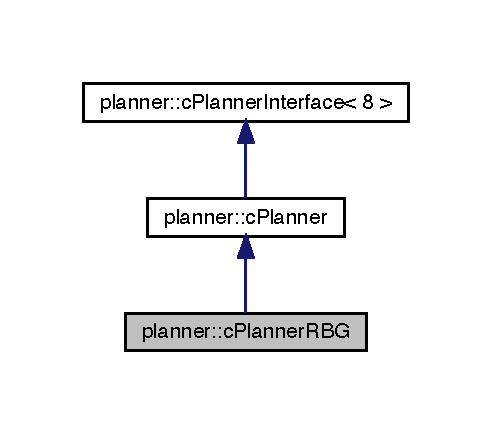
\includegraphics[width=236pt]{classplanner_1_1c_planner_r_b_g__inherit__graph}
\end{center}
\end{figure}


Collaboration diagram for planner\+:\+:c\+Planner\+R\+BG\+:
\nopagebreak
\begin{figure}[H]
\begin{center}
\leavevmode
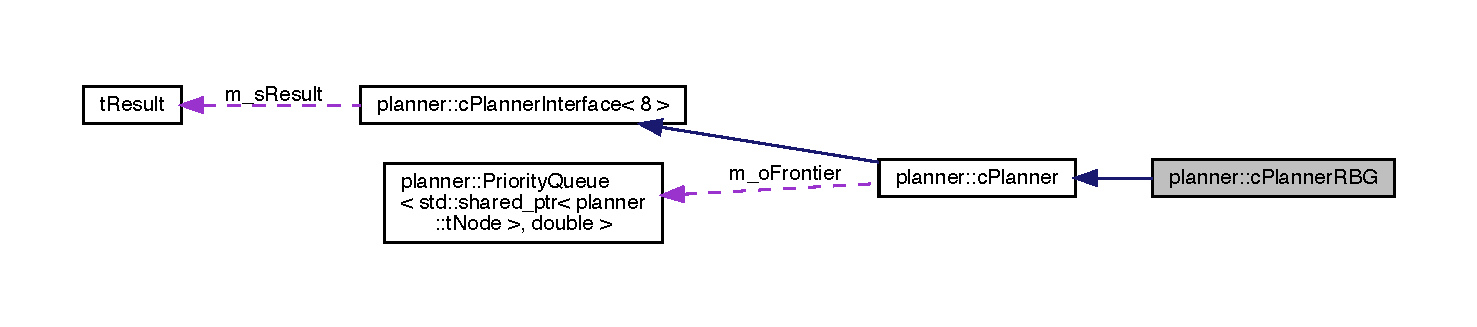
\includegraphics[width=350pt]{classplanner_1_1c_planner_r_b_g__coll__graph}
\end{center}
\end{figure}
\subsection*{Public Member Functions}
\begin{DoxyCompactItemize}
\item 
\mbox{\hyperlink{classplanner_1_1c_planner_r_b_g_a91296b98e64effc16f38e2430746d94d}{c\+Planner\+R\+BG}} (std\+::shared\+\_\+ptr$<$ \mbox{\hyperlink{classplanner_1_1c_rover_interface}{c\+Rover\+Interface}}$<$ 8 $>$$>$ i\+\_\+po\+Rover, std\+::shared\+\_\+ptr$<$ \mbox{\hyperlink{classplanner_1_1c_graph}{c\+Graph}} $>$ i\+\_\+o\+Map)
\begin{DoxyCompactList}\small\item\em Initializes member variables m\+\_\+po\+Rover and m\+\_\+o\+Map and calls \mbox{\hyperlink{classplanner_1_1c_planner_a2e5a745f83f903662eff914d8beddb5e}{Calculate\+Consistency\+Factor()}}. \end{DoxyCompactList}\item 
\mbox{\Hypertarget{classplanner_1_1c_planner_r_b_g_ad582fdf21ae0d86a23e9c25546b66f0e}\label{classplanner_1_1c_planner_r_b_g_ad582fdf21ae0d86a23e9c25546b66f0e}} 
\mbox{\hyperlink{classplanner_1_1c_planner_r_b_g_ad582fdf21ae0d86a23e9c25546b66f0e}{$\sim$c\+Planner\+R\+BG}} ()
\begin{DoxyCompactList}\small\item\em Destructor to delete the allocated memory. \end{DoxyCompactList}\item 
\mbox{\hyperlink{structt_result}{t\+Result}} \mbox{\hyperlink{classplanner_1_1c_planner_r_b_g_a0bbd752702da582a47dbd153c0065eb5}{Plan}} () override
\begin{DoxyCompactList}\small\item\em Override of the base interface \mbox{\hyperlink{classplanner_1_1c_planner_interface}{c\+Planner\+Interface}}, which invokes the A\+Star() search algorithm. \end{DoxyCompactList}\item 
{\footnotesize template$<$typename T\+Cost\+So\+Far , typename T\+Came\+From $>$ }\\void \mbox{\hyperlink{classplanner_1_1c_planner_r_b_g_a1af74d398b286f1e05e6ade495efbbd0}{Reconstruct\+Path}} (T\+Cost\+So\+Far \&\&i\+\_\+cost\+\_\+so\+\_\+far, T\+Came\+From \&\&i\+\_\+came\+\_\+from)
\begin{DoxyCompactList}\small\item\em Given the node i\+\_\+ps\+Node the overrides map m\+\_\+po\+Overrides is updated for displaying the path. \end{DoxyCompactList}\end{DoxyCompactItemize}
\subsection*{Additional Inherited Members}


\subsection{Detailed Description}
Extends the planner class to implement A$\ast$ from Wikipedia. 

\subsection{Constructor \& Destructor Documentation}
\mbox{\Hypertarget{classplanner_1_1c_planner_r_b_g_a91296b98e64effc16f38e2430746d94d}\label{classplanner_1_1c_planner_r_b_g_a91296b98e64effc16f38e2430746d94d}} 
\index{planner\+::c\+Planner\+R\+BG@{planner\+::c\+Planner\+R\+BG}!c\+Planner\+R\+BG@{c\+Planner\+R\+BG}}
\index{c\+Planner\+R\+BG@{c\+Planner\+R\+BG}!planner\+::c\+Planner\+R\+BG@{planner\+::c\+Planner\+R\+BG}}
\subsubsection{\texorpdfstring{c\+Planner\+R\+B\+G()}{cPlannerRBG()}}
{\footnotesize\ttfamily planner\+::c\+Planner\+R\+B\+G\+::c\+Planner\+R\+BG (\begin{DoxyParamCaption}\item[{std\+::shared\+\_\+ptr$<$ \mbox{\hyperlink{classplanner_1_1c_rover_interface}{c\+Rover\+Interface}}$<$ 8 $>$$>$}]{i\+\_\+po\+Rover,  }\item[{std\+::shared\+\_\+ptr$<$ \mbox{\hyperlink{classplanner_1_1c_graph}{c\+Graph}} $>$}]{i\+\_\+o\+Map }\end{DoxyParamCaption})}



Initializes member variables m\+\_\+po\+Rover and m\+\_\+o\+Map and calls \mbox{\hyperlink{classplanner_1_1c_planner_a2e5a745f83f903662eff914d8beddb5e}{Calculate\+Consistency\+Factor()}}. 

The 

\subsection{Member Function Documentation}
\mbox{\Hypertarget{classplanner_1_1c_planner_r_b_g_a0bbd752702da582a47dbd153c0065eb5}\label{classplanner_1_1c_planner_r_b_g_a0bbd752702da582a47dbd153c0065eb5}} 
\index{planner\+::c\+Planner\+R\+BG@{planner\+::c\+Planner\+R\+BG}!Plan@{Plan}}
\index{Plan@{Plan}!planner\+::c\+Planner\+R\+BG@{planner\+::c\+Planner\+R\+BG}}
\subsubsection{\texorpdfstring{Plan()}{Plan()}}
{\footnotesize\ttfamily \mbox{\hyperlink{structt_result}{t\+Result}} planner\+::c\+Planner\+R\+B\+G\+::\+Plan (\begin{DoxyParamCaption}{ }\end{DoxyParamCaption})\hspace{0.3cm}{\ttfamily [override]}, {\ttfamily [virtual]}}



Override of the base interface \mbox{\hyperlink{classplanner_1_1c_planner_interface}{c\+Planner\+Interface}}, which invokes the A\+Star() search algorithm. 

\begin{DoxyReturn}{Returns}
the time to travel from start to goal if it was found. Otherwise -\/1 is returned. 
\end{DoxyReturn}


Reimplemented from \mbox{\hyperlink{classplanner_1_1c_planner_a21230c015260b9fc34ad2f239592470e}{planner\+::c\+Planner}}.

\mbox{\Hypertarget{classplanner_1_1c_planner_r_b_g_a1af74d398b286f1e05e6ade495efbbd0}\label{classplanner_1_1c_planner_r_b_g_a1af74d398b286f1e05e6ade495efbbd0}} 
\index{planner\+::c\+Planner\+R\+BG@{planner\+::c\+Planner\+R\+BG}!Reconstruct\+Path@{Reconstruct\+Path}}
\index{Reconstruct\+Path@{Reconstruct\+Path}!planner\+::c\+Planner\+R\+BG@{planner\+::c\+Planner\+R\+BG}}
\subsubsection{\texorpdfstring{Reconstruct\+Path()}{ReconstructPath()}}
{\footnotesize\ttfamily template$<$typename T\+Cost\+So\+Far , typename T\+Came\+From $>$ \\
void planner\+::c\+Planner\+R\+B\+G\+::\+Reconstruct\+Path (\begin{DoxyParamCaption}\item[{T\+Cost\+So\+Far \&\&}]{i\+\_\+cost\+\_\+so\+\_\+far,  }\item[{T\+Came\+From \&\&}]{i\+\_\+came\+\_\+from }\end{DoxyParamCaption})}



Given the node i\+\_\+ps\+Node the overrides map m\+\_\+po\+Overrides is updated for displaying the path. 

Traversing a path takes place using the m\+\_\+ps\+Parent field of the \mbox{\hyperlink{structplanner_1_1t_node}{t\+Node}} struct. 
\begin{DoxyParams}[1]{Parameters}
\mbox{\tt in}  & {\em i\+\_\+ps\+Node} & Goal node or any other which is traversed back \\
\hline
\end{DoxyParams}
Reconstruct the path by going backward from the goal location

Set the cost (time) it takes to get to the goal

Update cumulative elevation

Store path in overrides

Check if the current node is the start node

Move towards the start

Update cumulative elevation

Store path in overrides 

The documentation for this class was generated from the following files\+:\begin{DoxyCompactItemize}
\item 
/\+Users/fjp/git/bachelor/planner/include/planner\+\_\+rbg.\+h\item 
/\+Users/fjp/git/bachelor/planner/src/planner\+\_\+rbg.\+cpp\end{DoxyCompactItemize}

\hypertarget{classc_planner_test}{}\section{c\+Planner\+Test Class Reference}
\label{classc_planner_test}\index{c\+Planner\+Test@{c\+Planner\+Test}}


The fixture for testing class \mbox{\hyperlink{classc_planner_test}{c\+Planner\+Test}}.  




{\ttfamily \#include $<$test\+\_\+fixture.\+h$>$}

Inheritance diagram for c\+Planner\+Test\+:\begin{figure}[H]
\begin{center}
\leavevmode
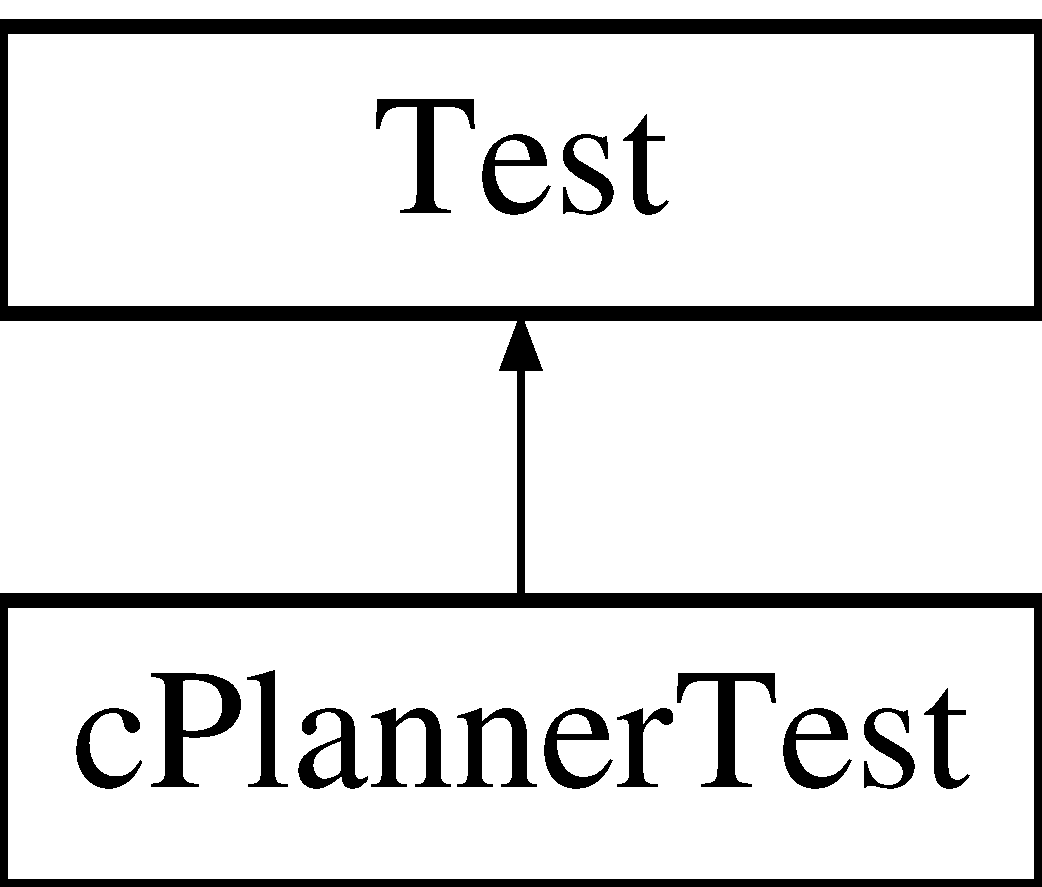
\includegraphics[height=2.000000cm]{classc_planner_test}
\end{center}
\end{figure}
\subsection*{Protected Member Functions}
\begin{DoxyCompactItemize}
\item 
void \mbox{\hyperlink{classc_planner_test_af8a0f625c6cb4dffc1ea3182332e53c6}{Read\+Data}} (std\+::string i\+\_\+str\+Elevation, std\+::string i\+\_\+str\+Overrides)
\item 
\mbox{\Hypertarget{classc_planner_test_ac1aac6152ea3ac86c5205fd8f0835d0c}\label{classc_planner_test_ac1aac6152ea3ac86c5205fd8f0835d0c}} 
void {\bfseries Init\+Island\+Map} ()
\item 
\mbox{\Hypertarget{classc_planner_test_a88ad8b0e63c66a9d94c7606aa67ef20d}\label{classc_planner_test_a88ad8b0e63c66a9d94c7606aa67ef20d}} 
void {\bfseries Set\+Up} () override
\item 
void \mbox{\hyperlink{classc_planner_test_a1e8b184185494cae8444fb7d5f846334}{Create\+Simple\+Map\+With\+Water}} ()
\item 
\mbox{\Hypertarget{classc_planner_test_aa55c78961deacf34543933e12cd82000}\label{classc_planner_test_aa55c78961deacf34543933e12cd82000}} 
void {\bfseries Init\+Simple\+Map\+With\+Water} ()
\item 
void \mbox{\hyperlink{classc_planner_test_a3d08d274ae12fbecd664ec70b4d6dfa3}{Create\+Simple\+Map\+With\+Elevation}} ()
\item 
\mbox{\Hypertarget{classc_planner_test_a59339eef13103205b18ab2f1b1f59d7e}\label{classc_planner_test_a59339eef13103205b18ab2f1b1f59d7e}} 
void {\bfseries Init\+Simple\+Map\+With\+Elevation} ()
\item 
void \mbox{\hyperlink{classc_planner_test_adc6dedb45d227191f0c87843a182d802}{Create\+Rover}} (const t\+Location \&i\+\_\+s\+Start, const t\+Location \&i\+\_\+s\+Goal)
\item 
\mbox{\Hypertarget{classc_planner_test_ae7db6ebf867e3ba6bf8adaaca636f064}\label{classc_planner_test_ae7db6ebf867e3ba6bf8adaaca636f064}} 
void {\bfseries Tear\+Down} () override
\item 
void \mbox{\hyperlink{classc_planner_test_af8a0f625c6cb4dffc1ea3182332e53c6}{Read\+Data}} (std\+::string i\+\_\+str\+Elevation, std\+::string i\+\_\+str\+Overrides)
\item 
\mbox{\Hypertarget{classc_planner_test_ac1aac6152ea3ac86c5205fd8f0835d0c}\label{classc_planner_test_ac1aac6152ea3ac86c5205fd8f0835d0c}} 
void {\bfseries Init\+Island\+Map} ()
\item 
\mbox{\Hypertarget{classc_planner_test_a88ad8b0e63c66a9d94c7606aa67ef20d}\label{classc_planner_test_a88ad8b0e63c66a9d94c7606aa67ef20d}} 
void {\bfseries Set\+Up} () override
\item 
void \mbox{\hyperlink{classc_planner_test_a1e8b184185494cae8444fb7d5f846334}{Create\+Simple\+Map\+With\+Water}} ()
\item 
\mbox{\Hypertarget{classc_planner_test_aa55c78961deacf34543933e12cd82000}\label{classc_planner_test_aa55c78961deacf34543933e12cd82000}} 
void {\bfseries Init\+Simple\+Map\+With\+Water} ()
\item 
void \mbox{\hyperlink{classc_planner_test_a3d08d274ae12fbecd664ec70b4d6dfa3}{Create\+Simple\+Map\+With\+Elevation}} ()
\item 
\mbox{\Hypertarget{classc_planner_test_a59339eef13103205b18ab2f1b1f59d7e}\label{classc_planner_test_a59339eef13103205b18ab2f1b1f59d7e}} 
void {\bfseries Init\+Simple\+Map\+With\+Elevation} ()
\item 
void \mbox{\hyperlink{classc_planner_test_adc6dedb45d227191f0c87843a182d802}{Create\+Rover}} (const t\+Location \&i\+\_\+s\+Start, const t\+Location \&i\+\_\+s\+Goal)
\item 
\mbox{\Hypertarget{classc_planner_test_ae7db6ebf867e3ba6bf8adaaca636f064}\label{classc_planner_test_ae7db6ebf867e3ba6bf8adaaca636f064}} 
void {\bfseries Tear\+Down} () override
\end{DoxyCompactItemize}
\subsection*{Protected Attributes}
\begin{DoxyCompactItemize}
\item 
\mbox{\Hypertarget{classc_planner_test_a2c83ae3b350736b9005788134eb023e2}\label{classc_planner_test_a2c83ae3b350736b9005788134eb023e2}} 
std\+::vector$<$ uint8\+\_\+t $>$ {\bfseries m\+\_\+o\+Elevation}
\item 
\mbox{\Hypertarget{classc_planner_test_a30d78247a35a834582a09a4b9585b28a}\label{classc_planner_test_a30d78247a35a834582a09a4b9585b28a}} 
std\+::vector$<$ uint8\+\_\+t $>$ {\bfseries m\+\_\+o\+Overrides}
\item 
\mbox{\Hypertarget{classc_planner_test_a15fb3c0b9281c70b51654f88799c0c07}\label{classc_planner_test_a15fb3c0b9281c70b51654f88799c0c07}} 
std\+::shared\+\_\+ptr$<$ c\+Audi\+Rover $>$ {\bfseries m\+\_\+po\+Audi\+Rover}
\item 
\mbox{\Hypertarget{classc_planner_test_a1d1e9b95d362b2f8488c988e9f05583b}\label{classc_planner_test_a1d1e9b95d362b2f8488c988e9f05583b}} 
int {\bfseries m\+\_\+n\+Image\+Dim}
\end{DoxyCompactItemize}
\subsection*{Additional Inherited Members}


\subsection{Detailed Description}
The fixture for testing class \mbox{\hyperlink{classc_planner_test}{c\+Planner\+Test}}. 

\subsection{Member Function Documentation}
\mbox{\Hypertarget{classc_planner_test_adc6dedb45d227191f0c87843a182d802}\label{classc_planner_test_adc6dedb45d227191f0c87843a182d802}} 
\index{c\+Planner\+Test@{c\+Planner\+Test}!Create\+Rover@{Create\+Rover}}
\index{Create\+Rover@{Create\+Rover}!c\+Planner\+Test@{c\+Planner\+Test}}
\subsubsection{\texorpdfstring{Create\+Rover()}{CreateRover()}\hspace{0.1cm}{\footnotesize\ttfamily [1/2]}}
{\footnotesize\ttfamily void c\+Planner\+Test\+::\+Create\+Rover (\begin{DoxyParamCaption}\item[{const t\+Location \&}]{i\+\_\+s\+Start,  }\item[{const t\+Location \&}]{i\+\_\+s\+Goal }\end{DoxyParamCaption})\hspace{0.3cm}{\ttfamily [inline]}, {\ttfamily [protected]}}

Create Audi rover

Bachelor calls Audi rover \mbox{\Hypertarget{classc_planner_test_adc6dedb45d227191f0c87843a182d802}\label{classc_planner_test_adc6dedb45d227191f0c87843a182d802}} 
\index{c\+Planner\+Test@{c\+Planner\+Test}!Create\+Rover@{Create\+Rover}}
\index{Create\+Rover@{Create\+Rover}!c\+Planner\+Test@{c\+Planner\+Test}}
\subsubsection{\texorpdfstring{Create\+Rover()}{CreateRover()}\hspace{0.1cm}{\footnotesize\ttfamily [2/2]}}
{\footnotesize\ttfamily void c\+Planner\+Test\+::\+Create\+Rover (\begin{DoxyParamCaption}\item[{const t\+Location \&}]{i\+\_\+s\+Start,  }\item[{const t\+Location \&}]{i\+\_\+s\+Goal }\end{DoxyParamCaption})\hspace{0.3cm}{\ttfamily [inline]}, {\ttfamily [protected]}}

Create Audi rover

Bachelor calls Audi rover \mbox{\Hypertarget{classc_planner_test_a3d08d274ae12fbecd664ec70b4d6dfa3}\label{classc_planner_test_a3d08d274ae12fbecd664ec70b4d6dfa3}} 
\index{c\+Planner\+Test@{c\+Planner\+Test}!Create\+Simple\+Map\+With\+Elevation@{Create\+Simple\+Map\+With\+Elevation}}
\index{Create\+Simple\+Map\+With\+Elevation@{Create\+Simple\+Map\+With\+Elevation}!c\+Planner\+Test@{c\+Planner\+Test}}
\subsubsection{\texorpdfstring{Create\+Simple\+Map\+With\+Elevation()}{CreateSimpleMapWithElevation()}\hspace{0.1cm}{\footnotesize\ttfamily [1/2]}}
{\footnotesize\ttfamily void c\+Planner\+Test\+::\+Create\+Simple\+Map\+With\+Elevation (\begin{DoxyParamCaption}{ }\end{DoxyParamCaption})\hspace{0.3cm}{\ttfamily [inline]}, {\ttfamily [protected]}}

Prepare to read elevation and overrides data \mbox{\Hypertarget{classc_planner_test_a3d08d274ae12fbecd664ec70b4d6dfa3}\label{classc_planner_test_a3d08d274ae12fbecd664ec70b4d6dfa3}} 
\index{c\+Planner\+Test@{c\+Planner\+Test}!Create\+Simple\+Map\+With\+Elevation@{Create\+Simple\+Map\+With\+Elevation}}
\index{Create\+Simple\+Map\+With\+Elevation@{Create\+Simple\+Map\+With\+Elevation}!c\+Planner\+Test@{c\+Planner\+Test}}
\subsubsection{\texorpdfstring{Create\+Simple\+Map\+With\+Elevation()}{CreateSimpleMapWithElevation()}\hspace{0.1cm}{\footnotesize\ttfamily [2/2]}}
{\footnotesize\ttfamily void c\+Planner\+Test\+::\+Create\+Simple\+Map\+With\+Elevation (\begin{DoxyParamCaption}{ }\end{DoxyParamCaption})\hspace{0.3cm}{\ttfamily [inline]}, {\ttfamily [protected]}}

Prepare to read elevation and overrides data \mbox{\Hypertarget{classc_planner_test_a1e8b184185494cae8444fb7d5f846334}\label{classc_planner_test_a1e8b184185494cae8444fb7d5f846334}} 
\index{c\+Planner\+Test@{c\+Planner\+Test}!Create\+Simple\+Map\+With\+Water@{Create\+Simple\+Map\+With\+Water}}
\index{Create\+Simple\+Map\+With\+Water@{Create\+Simple\+Map\+With\+Water}!c\+Planner\+Test@{c\+Planner\+Test}}
\subsubsection{\texorpdfstring{Create\+Simple\+Map\+With\+Water()}{CreateSimpleMapWithWater()}\hspace{0.1cm}{\footnotesize\ttfamily [1/2]}}
{\footnotesize\ttfamily void c\+Planner\+Test\+::\+Create\+Simple\+Map\+With\+Water (\begin{DoxyParamCaption}{ }\end{DoxyParamCaption})\hspace{0.3cm}{\ttfamily [inline]}, {\ttfamily [protected]}}

Prepare to read elevation and overrides data \mbox{\Hypertarget{classc_planner_test_a1e8b184185494cae8444fb7d5f846334}\label{classc_planner_test_a1e8b184185494cae8444fb7d5f846334}} 
\index{c\+Planner\+Test@{c\+Planner\+Test}!Create\+Simple\+Map\+With\+Water@{Create\+Simple\+Map\+With\+Water}}
\index{Create\+Simple\+Map\+With\+Water@{Create\+Simple\+Map\+With\+Water}!c\+Planner\+Test@{c\+Planner\+Test}}
\subsubsection{\texorpdfstring{Create\+Simple\+Map\+With\+Water()}{CreateSimpleMapWithWater()}\hspace{0.1cm}{\footnotesize\ttfamily [2/2]}}
{\footnotesize\ttfamily void c\+Planner\+Test\+::\+Create\+Simple\+Map\+With\+Water (\begin{DoxyParamCaption}{ }\end{DoxyParamCaption})\hspace{0.3cm}{\ttfamily [inline]}, {\ttfamily [protected]}}

Prepare to read elevation and overrides data \mbox{\Hypertarget{classc_planner_test_af8a0f625c6cb4dffc1ea3182332e53c6}\label{classc_planner_test_af8a0f625c6cb4dffc1ea3182332e53c6}} 
\index{c\+Planner\+Test@{c\+Planner\+Test}!Read\+Data@{Read\+Data}}
\index{Read\+Data@{Read\+Data}!c\+Planner\+Test@{c\+Planner\+Test}}
\subsubsection{\texorpdfstring{Read\+Data()}{ReadData()}\hspace{0.1cm}{\footnotesize\ttfamily [1/2]}}
{\footnotesize\ttfamily void c\+Planner\+Test\+::\+Read\+Data (\begin{DoxyParamCaption}\item[{std\+::string}]{i\+\_\+str\+Elevation,  }\item[{std\+::string}]{i\+\_\+str\+Overrides }\end{DoxyParamCaption})\hspace{0.3cm}{\ttfamily [inline]}, {\ttfamily [protected]}}

Prepare to read elevation and overrides data \mbox{\Hypertarget{classc_planner_test_af8a0f625c6cb4dffc1ea3182332e53c6}\label{classc_planner_test_af8a0f625c6cb4dffc1ea3182332e53c6}} 
\index{c\+Planner\+Test@{c\+Planner\+Test}!Read\+Data@{Read\+Data}}
\index{Read\+Data@{Read\+Data}!c\+Planner\+Test@{c\+Planner\+Test}}
\subsubsection{\texorpdfstring{Read\+Data()}{ReadData()}\hspace{0.1cm}{\footnotesize\ttfamily [2/2]}}
{\footnotesize\ttfamily void c\+Planner\+Test\+::\+Read\+Data (\begin{DoxyParamCaption}\item[{std\+::string}]{i\+\_\+str\+Elevation,  }\item[{std\+::string}]{i\+\_\+str\+Overrides }\end{DoxyParamCaption})\hspace{0.3cm}{\ttfamily [inline]}, {\ttfamily [protected]}}

Prepare to read elevation and overrides data 

The documentation for this class was generated from the following file\+:\begin{DoxyCompactItemize}
\item 
/\+Users/fjp/git/bachelor/bachelor-\/master\+\_\+updated\+\_\+vfinal/planner/test/test\+\_\+fixture.\+h\end{DoxyCompactItemize}

\hypertarget{classplanner_1_1c_planner_wiki}{}\section{planner\+:\+:c\+Planner\+Wiki Class Reference}
\label{classplanner_1_1c_planner_wiki}\index{planner\+::c\+Planner\+Wiki@{planner\+::c\+Planner\+Wiki}}


Extends the planner class to implement A$\ast$ from Wikipedia.  




{\ttfamily \#include $<$planner\+\_\+wiki.\+h$>$}

Inheritance diagram for planner\+:\+:c\+Planner\+Wiki\+:\begin{figure}[H]
\begin{center}
\leavevmode
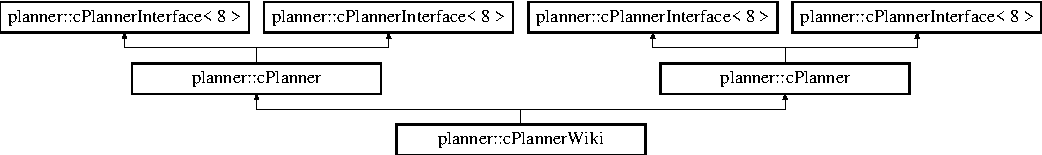
\includegraphics[height=2.089552cm]{classplanner_1_1c_planner_wiki}
\end{center}
\end{figure}
\subsection*{Public Member Functions}
\begin{DoxyCompactItemize}
\item 
\mbox{\hyperlink{classplanner_1_1c_planner_wiki_aed6ae97e85a338e082ec2879629f0f3b}{c\+Planner\+Wiki}} (std\+::shared\+\_\+ptr$<$ \mbox{\hyperlink{classplanner_1_1c_rover_interface}{c\+Rover\+Interface}}$<$ 8 $>$$>$ i\+\_\+po\+Rover, std\+::shared\+\_\+ptr$<$ \mbox{\hyperlink{classplanner_1_1c_graph}{c\+Graph}} $>$ i\+\_\+o\+Map)
\begin{DoxyCompactList}\small\item\em Initializes member variables m\+\_\+po\+Rover and m\+\_\+o\+Map and calls \mbox{\hyperlink{classplanner_1_1c_planner_a2e5a745f83f903662eff914d8beddb5e}{Calculate\+Consistency\+Factor()}}. \end{DoxyCompactList}\item 
\mbox{\Hypertarget{classplanner_1_1c_planner_wiki_ab9f2b825a5b1e0bd2e33271f25c812be}\label{classplanner_1_1c_planner_wiki_ab9f2b825a5b1e0bd2e33271f25c812be}} 
\mbox{\hyperlink{classplanner_1_1c_planner_wiki_ab9f2b825a5b1e0bd2e33271f25c812be}{$\sim$c\+Planner\+Wiki}} ()
\begin{DoxyCompactList}\small\item\em Destructor to delete the allocated memory. \end{DoxyCompactList}\item 
\mbox{\hyperlink{structt_result}{t\+Result}} \mbox{\hyperlink{classplanner_1_1c_planner_wiki_a9d18be721400b51162ff463ab11d1721}{Plan}} () override
\begin{DoxyCompactList}\small\item\em Override of the base interface \mbox{\hyperlink{classplanner_1_1c_planner_interface}{c\+Planner\+Interface}}, which invokes the \mbox{\hyperlink{classplanner_1_1c_planner_wiki_aa673ebc2b1b43af3b13fb0c958c5f2e4}{A\+Star()}} search algorithm. \end{DoxyCompactList}\item 
{\footnotesize template$<$typename T\+Cost\+So\+Far , typename T\+Came\+From $>$ }\\void \mbox{\hyperlink{classplanner_1_1c_planner_wiki_a049e5c4a9540fecbe82a0648f771bbd2}{Reconstruct\+Path}} (T\+Cost\+So\+Far \&\&i\+\_\+cost\+\_\+so\+\_\+far, T\+Came\+From \&\&i\+\_\+came\+\_\+from)
\begin{DoxyCompactList}\small\item\em Given the node i\+\_\+ps\+Node the overrides map m\+\_\+po\+Overrides is updated for displaying the path. \end{DoxyCompactList}\item 
\mbox{\hyperlink{classplanner_1_1c_planner_wiki_aed6ae97e85a338e082ec2879629f0f3b}{c\+Planner\+Wiki}} (std\+::shared\+\_\+ptr$<$ \mbox{\hyperlink{classplanner_1_1c_rover_interface}{c\+Rover\+Interface}}$<$ 8 $>$$>$ i\+\_\+po\+Rover, std\+::shared\+\_\+ptr$<$ \mbox{\hyperlink{classplanner_1_1c_graph}{c\+Graph}} $>$ i\+\_\+o\+Map)
\begin{DoxyCompactList}\small\item\em Initializes member variables m\+\_\+po\+Rover and m\+\_\+o\+Map and calls \mbox{\hyperlink{classplanner_1_1c_planner_a2e5a745f83f903662eff914d8beddb5e}{Calculate\+Consistency\+Factor()}}. \end{DoxyCompactList}\item 
\mbox{\Hypertarget{classplanner_1_1c_planner_wiki_ab9f2b825a5b1e0bd2e33271f25c812be}\label{classplanner_1_1c_planner_wiki_ab9f2b825a5b1e0bd2e33271f25c812be}} 
\mbox{\hyperlink{classplanner_1_1c_planner_wiki_ab9f2b825a5b1e0bd2e33271f25c812be}{$\sim$c\+Planner\+Wiki}} ()
\begin{DoxyCompactList}\small\item\em Destructor to delete the allocated memory. \end{DoxyCompactList}\item 
\mbox{\hyperlink{structt_result}{t\+Result}} \mbox{\hyperlink{classplanner_1_1c_planner_wiki_a9d18be721400b51162ff463ab11d1721}{Plan}} () override
\begin{DoxyCompactList}\small\item\em Override of the base interface \mbox{\hyperlink{classplanner_1_1c_planner_interface}{c\+Planner\+Interface}}, which invokes the \mbox{\hyperlink{classplanner_1_1c_planner_wiki_aa673ebc2b1b43af3b13fb0c958c5f2e4}{A\+Star()}} search algorithm. \end{DoxyCompactList}\item 
{\footnotesize template$<$typename T\+Cost\+So\+Far , typename T\+Came\+From $>$ }\\void \mbox{\hyperlink{classplanner_1_1c_planner_wiki_a049e5c4a9540fecbe82a0648f771bbd2}{Reconstruct\+Path}} (T\+Cost\+So\+Far \&\&i\+\_\+cost\+\_\+so\+\_\+far, T\+Came\+From \&\&i\+\_\+came\+\_\+from)
\begin{DoxyCompactList}\small\item\em Given the node i\+\_\+ps\+Node the overrides map m\+\_\+po\+Overrides is updated for displaying the path. \end{DoxyCompactList}\end{DoxyCompactItemize}
\subsection*{Protected Member Functions}
\begin{DoxyCompactItemize}
\item 
\mbox{\hyperlink{structt_result}{t\+Result}} \mbox{\hyperlink{classplanner_1_1c_planner_wiki_aa673ebc2b1b43af3b13fb0c958c5f2e4}{A\+Star}} ()
\item 
\mbox{\Hypertarget{classplanner_1_1c_planner_wiki_aa673ebc2b1b43af3b13fb0c958c5f2e4}\label{classplanner_1_1c_planner_wiki_aa673ebc2b1b43af3b13fb0c958c5f2e4}} 
\mbox{\hyperlink{structt_result}{t\+Result}} {\bfseries A\+Star} ()
\end{DoxyCompactItemize}
\subsection*{Additional Inherited Members}


\subsection{Detailed Description}
Extends the planner class to implement A$\ast$ from Wikipedia. 

\subsection{Constructor \& Destructor Documentation}
\mbox{\Hypertarget{classplanner_1_1c_planner_wiki_aed6ae97e85a338e082ec2879629f0f3b}\label{classplanner_1_1c_planner_wiki_aed6ae97e85a338e082ec2879629f0f3b}} 
\index{planner\+::c\+Planner\+Wiki@{planner\+::c\+Planner\+Wiki}!c\+Planner\+Wiki@{c\+Planner\+Wiki}}
\index{c\+Planner\+Wiki@{c\+Planner\+Wiki}!planner\+::c\+Planner\+Wiki@{planner\+::c\+Planner\+Wiki}}
\subsubsection{\texorpdfstring{c\+Planner\+Wiki()}{cPlannerWiki()}\hspace{0.1cm}{\footnotesize\ttfamily [1/2]}}
{\footnotesize\ttfamily planner\+::c\+Planner\+Wiki\+::c\+Planner\+Wiki (\begin{DoxyParamCaption}\item[{std\+::shared\+\_\+ptr$<$ \mbox{\hyperlink{classplanner_1_1c_rover_interface}{c\+Rover\+Interface}}$<$ 8 $>$$>$}]{i\+\_\+po\+Rover,  }\item[{std\+::shared\+\_\+ptr$<$ \mbox{\hyperlink{classplanner_1_1c_graph}{c\+Graph}} $>$}]{i\+\_\+o\+Map }\end{DoxyParamCaption})}



Initializes member variables m\+\_\+po\+Rover and m\+\_\+o\+Map and calls \mbox{\hyperlink{classplanner_1_1c_planner_a2e5a745f83f903662eff914d8beddb5e}{Calculate\+Consistency\+Factor()}}. 

The \mbox{\Hypertarget{classplanner_1_1c_planner_wiki_aed6ae97e85a338e082ec2879629f0f3b}\label{classplanner_1_1c_planner_wiki_aed6ae97e85a338e082ec2879629f0f3b}} 
\index{planner\+::c\+Planner\+Wiki@{planner\+::c\+Planner\+Wiki}!c\+Planner\+Wiki@{c\+Planner\+Wiki}}
\index{c\+Planner\+Wiki@{c\+Planner\+Wiki}!planner\+::c\+Planner\+Wiki@{planner\+::c\+Planner\+Wiki}}
\subsubsection{\texorpdfstring{c\+Planner\+Wiki()}{cPlannerWiki()}\hspace{0.1cm}{\footnotesize\ttfamily [2/2]}}
{\footnotesize\ttfamily planner\+::c\+Planner\+Wiki\+::c\+Planner\+Wiki (\begin{DoxyParamCaption}\item[{std\+::shared\+\_\+ptr$<$ \mbox{\hyperlink{classplanner_1_1c_rover_interface}{c\+Rover\+Interface}}$<$ 8 $>$$>$}]{i\+\_\+po\+Rover,  }\item[{std\+::shared\+\_\+ptr$<$ \mbox{\hyperlink{classplanner_1_1c_graph}{c\+Graph}} $>$}]{i\+\_\+o\+Map }\end{DoxyParamCaption})}



Initializes member variables m\+\_\+po\+Rover and m\+\_\+o\+Map and calls \mbox{\hyperlink{classplanner_1_1c_planner_a2e5a745f83f903662eff914d8beddb5e}{Calculate\+Consistency\+Factor()}}. 

The 

\subsection{Member Function Documentation}
\mbox{\Hypertarget{classplanner_1_1c_planner_wiki_aa673ebc2b1b43af3b13fb0c958c5f2e4}\label{classplanner_1_1c_planner_wiki_aa673ebc2b1b43af3b13fb0c958c5f2e4}} 
\index{planner\+::c\+Planner\+Wiki@{planner\+::c\+Planner\+Wiki}!A\+Star@{A\+Star}}
\index{A\+Star@{A\+Star}!planner\+::c\+Planner\+Wiki@{planner\+::c\+Planner\+Wiki}}
\subsubsection{\texorpdfstring{A\+Star()}{AStar()}}
{\footnotesize\ttfamily \mbox{\hyperlink{structt_result}{t\+Result}} planner\+::c\+Planner\+Wiki\+::\+A\+Star (\begin{DoxyParamCaption}{ }\end{DoxyParamCaption})\hspace{0.3cm}{\ttfamily [protected]}}

The set of nodes already evaluated. Implemented as 2d array filled with 0s and start element set to 1.

The set of currently discovered nodes that are not evaluated yet. Initially, only the start node is known. ~\newline
~\newline
~\newline
~\newline
~\newline
~\newline
~\newline
~\newline
~\newline
~\newline
~\newline
~\newline
~\newline
~\newline
~\newline
~\newline
 Defined the simplified start node

For each node, which action it can most efficiently be reached from. If a node can be reached from many nodes, action will eventually contain the most efficient previous step. ~\newline
~\newline
~\newline
~\newline
~\newline
~\newline
~\newline
~\newline
~\newline
~\newline
~\newline
~\newline
~\newline
~\newline
 For each node, the cost of getting from the start node to that node.

The cost of going from start to start is zero.

Initialize result struct

While the goal is not found the problem is solvable

Resign if no values in the open list and you can\textquotesingle{}t expand anymore

Remove the node from the open priority queue having the lowest f\+Score value

Check if the goal is reached

Otherwise explore new locations

Add the current node to the set of nodes already evaluated

Perform each possible rover action on the current node

Check if the location of the next node lies within the map and is not on water. Ignore the neighbors which are already evaluated (closed\mbox{[}n\+X\+Next\mbox{]}\mbox{[}n\+Y\+Next\mbox{]} == 0). ~\newline
~\newline
~\newline
 The distance from start to a neighbor

Mark visited nodes

Check that heuristic never overestimates the true distance\+: Priority of a new node should never be lower than the priority of its parent.

The set of nodes already evaluated. Implemented as 2d array filled with 0s and start element set to 1.

The set of currently discovered nodes that are not evaluated yet. Initially, only the start node is known. ~\newline
~\newline
~\newline
~\newline
~\newline
~\newline
~\newline
~\newline
~\newline
~\newline
~\newline
~\newline
~\newline
~\newline
~\newline
~\newline
~\newline
 Defined the simplified start node

For each node, which action it can most efficiently be reached from. If a node can be reached from many nodes, action will eventually contain the most efficient previous step. ~\newline
~\newline
~\newline
~\newline
~\newline
~\newline
~\newline
~\newline
~\newline
~\newline
~\newline
~\newline
~\newline
~\newline
~\newline
 For each node, the cost of getting from the start node to that node.

The cost of going from start to start is zero.

Initialize result struct

While the goal is not found the problem is solvable

Resign if no values in the open list and you can\textquotesingle{}t expand anymore

Remove the node from the open priority queue having the lowest f\+Score value

Check if the goal is reached

Otherwise explore new locations

Add the current node to the set of nodes already evaluated

Perform each possible rover action on the current node

Check if the location of the next node lies within the map and is not on water. Ignore the neighbors which are already evaluated (closed\mbox{[}n\+X\+Next\mbox{]}\mbox{[}n\+Y\+Next\mbox{]} == 0). ~\newline
~\newline
~\newline
~\newline
 The distance from start to a neighbor

Mark visited nodes

Check that heuristic never overestimates the true distance\+: Priority of a new node should never be lower than the priority of its parent. ~\newline
 Move from the current node back to the start node \mbox{\Hypertarget{classplanner_1_1c_planner_wiki_a9d18be721400b51162ff463ab11d1721}\label{classplanner_1_1c_planner_wiki_a9d18be721400b51162ff463ab11d1721}} 
\index{planner\+::c\+Planner\+Wiki@{planner\+::c\+Planner\+Wiki}!Plan@{Plan}}
\index{Plan@{Plan}!planner\+::c\+Planner\+Wiki@{planner\+::c\+Planner\+Wiki}}
\subsubsection{\texorpdfstring{Plan()}{Plan()}\hspace{0.1cm}{\footnotesize\ttfamily [1/2]}}
{\footnotesize\ttfamily \mbox{\hyperlink{structt_result}{t\+Result}} planner\+::c\+Planner\+Wiki\+::\+Plan (\begin{DoxyParamCaption}{ }\end{DoxyParamCaption})\hspace{0.3cm}{\ttfamily [override]}, {\ttfamily [virtual]}}



Override of the base interface \mbox{\hyperlink{classplanner_1_1c_planner_interface}{c\+Planner\+Interface}}, which invokes the \mbox{\hyperlink{classplanner_1_1c_planner_wiki_aa673ebc2b1b43af3b13fb0c958c5f2e4}{A\+Star()}} search algorithm. 

\begin{DoxyReturn}{Returns}
the time to travel from start to goal if it was found. Otherwise -\/1 is returned. 
\end{DoxyReturn}


Reimplemented from \mbox{\hyperlink{classplanner_1_1c_planner_a21230c015260b9fc34ad2f239592470e}{planner\+::c\+Planner}}.

\mbox{\Hypertarget{classplanner_1_1c_planner_wiki_a9d18be721400b51162ff463ab11d1721}\label{classplanner_1_1c_planner_wiki_a9d18be721400b51162ff463ab11d1721}} 
\index{planner\+::c\+Planner\+Wiki@{planner\+::c\+Planner\+Wiki}!Plan@{Plan}}
\index{Plan@{Plan}!planner\+::c\+Planner\+Wiki@{planner\+::c\+Planner\+Wiki}}
\subsubsection{\texorpdfstring{Plan()}{Plan()}\hspace{0.1cm}{\footnotesize\ttfamily [2/2]}}
{\footnotesize\ttfamily \mbox{\hyperlink{structt_result}{t\+Result}} planner\+::c\+Planner\+Wiki\+::\+Plan (\begin{DoxyParamCaption}{ }\end{DoxyParamCaption})\hspace{0.3cm}{\ttfamily [override]}, {\ttfamily [virtual]}}



Override of the base interface \mbox{\hyperlink{classplanner_1_1c_planner_interface}{c\+Planner\+Interface}}, which invokes the \mbox{\hyperlink{classplanner_1_1c_planner_wiki_aa673ebc2b1b43af3b13fb0c958c5f2e4}{A\+Star()}} search algorithm. 

\begin{DoxyReturn}{Returns}
the time to travel from start to goal if it was found. Otherwise -\/1 is returned. 
\end{DoxyReturn}


Reimplemented from \mbox{\hyperlink{classplanner_1_1c_planner_a21230c015260b9fc34ad2f239592470e}{planner\+::c\+Planner}}.

\mbox{\Hypertarget{classplanner_1_1c_planner_wiki_a049e5c4a9540fecbe82a0648f771bbd2}\label{classplanner_1_1c_planner_wiki_a049e5c4a9540fecbe82a0648f771bbd2}} 
\index{planner\+::c\+Planner\+Wiki@{planner\+::c\+Planner\+Wiki}!Reconstruct\+Path@{Reconstruct\+Path}}
\index{Reconstruct\+Path@{Reconstruct\+Path}!planner\+::c\+Planner\+Wiki@{planner\+::c\+Planner\+Wiki}}
\subsubsection{\texorpdfstring{Reconstruct\+Path()}{ReconstructPath()}\hspace{0.1cm}{\footnotesize\ttfamily [1/2]}}
{\footnotesize\ttfamily template$<$typename T\+Cost\+So\+Far , typename T\+Came\+From $>$ \\
void planner\+::c\+Planner\+Wiki\+::\+Reconstruct\+Path (\begin{DoxyParamCaption}\item[{T\+Cost\+So\+Far \&\&}]{i\+\_\+cost\+\_\+so\+\_\+far,  }\item[{T\+Came\+From \&\&}]{i\+\_\+came\+\_\+from }\end{DoxyParamCaption})}



Given the node i\+\_\+ps\+Node the overrides map m\+\_\+po\+Overrides is updated for displaying the path. 

Traversing a path takes place using the m\+\_\+ps\+Parent field of the \mbox{\hyperlink{structplanner_1_1t_node}{t\+Node}} struct. 
\begin{DoxyParams}[1]{Parameters}
\mbox{\tt in}  & {\em i\+\_\+ps\+Node} & Goal node or any other which is traversed back \\
\hline
\end{DoxyParams}
Set the cost (time) it takes to get to the goal

Reconstruct the path by going backward

Update cumulative elevation

Store path in overrides

Check if the current node is the start node

Move towards the start

Update cumulative elevation

Store path in overrides

Set the cost (time) it takes to get to the goal

Reconstruct the path by going backward

Update cumulative elevation

Store path in overrides

Check if the current node is the start node

Move towards the start

Update cumulative elevation

Store path in overrides \mbox{\Hypertarget{classplanner_1_1c_planner_wiki_a049e5c4a9540fecbe82a0648f771bbd2}\label{classplanner_1_1c_planner_wiki_a049e5c4a9540fecbe82a0648f771bbd2}} 
\index{planner\+::c\+Planner\+Wiki@{planner\+::c\+Planner\+Wiki}!Reconstruct\+Path@{Reconstruct\+Path}}
\index{Reconstruct\+Path@{Reconstruct\+Path}!planner\+::c\+Planner\+Wiki@{planner\+::c\+Planner\+Wiki}}
\subsubsection{\texorpdfstring{Reconstruct\+Path()}{ReconstructPath()}\hspace{0.1cm}{\footnotesize\ttfamily [2/2]}}
{\footnotesize\ttfamily template$<$typename T\+Cost\+So\+Far , typename T\+Came\+From $>$ \\
void planner\+::c\+Planner\+Wiki\+::\+Reconstruct\+Path (\begin{DoxyParamCaption}\item[{T\+Cost\+So\+Far \&\&}]{i\+\_\+cost\+\_\+so\+\_\+far,  }\item[{T\+Came\+From \&\&}]{i\+\_\+came\+\_\+from }\end{DoxyParamCaption})}



Given the node i\+\_\+ps\+Node the overrides map m\+\_\+po\+Overrides is updated for displaying the path. 

Traversing a path takes place using the m\+\_\+ps\+Parent field of the \mbox{\hyperlink{structplanner_1_1t_node}{t\+Node}} struct. 
\begin{DoxyParams}[1]{Parameters}
\mbox{\tt in}  & {\em i\+\_\+ps\+Node} & Goal node or any other which is traversed back \\
\hline
\end{DoxyParams}


The documentation for this class was generated from the following files\+:\begin{DoxyCompactItemize}
\item 
/\+Users/fjp/git/bachelor/bachelor-\/master\+\_\+updated\+\_\+vfinal/planner/include/planner\+\_\+wiki.\+h\item 
/\+Users/fjp/git/bachelor/bachelor-\/master\+\_\+updated\+\_\+vfinal/planner/src/planner\+\_\+wiki.\+cpp\end{DoxyCompactItemize}

\hypertarget{classplanner_1_1c_rover_interface}{}\section{planner\+:\+:c\+Rover\+Interface$<$ Directions $>$ Class Template Reference}
\label{classplanner_1_1c_rover_interface}\index{planner\+::c\+Rover\+Interface$<$ Directions $>$@{planner\+::c\+Rover\+Interface$<$ Directions $>$}}


Forward declaration of interface \mbox{\hyperlink{classplanner_1_1c_rover_interface}{planner\+::c\+Rover\+Interface}}.  




{\ttfamily \#include $<$planner\+\_\+interface.\+h$>$}



Collaboration diagram for planner\+:\+:c\+Rover\+Interface$<$ Directions $>$\+:
\nopagebreak
\begin{figure}[H]
\begin{center}
\leavevmode
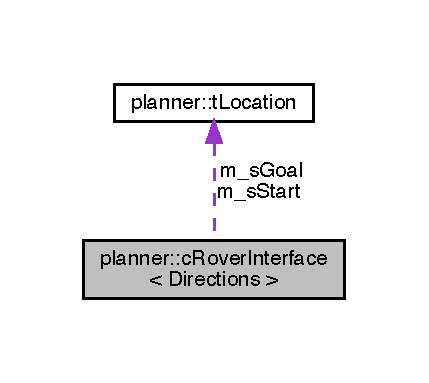
\includegraphics[width=206pt]{classplanner_1_1c_rover_interface__coll__graph}
\end{center}
\end{figure}
\subsection*{Public Member Functions}
\begin{DoxyCompactItemize}
\item 
\mbox{\Hypertarget{classplanner_1_1c_rover_interface_a7fedea18832ad850de1a2589fdca88b7}\label{classplanner_1_1c_rover_interface_a7fedea18832ad850de1a2589fdca88b7}} 
virtual std\+::shared\+\_\+ptr$<$ \mbox{\hyperlink{classplanner_1_1c_planner_interface}{c\+Planner\+Interface}}$<$ Directions $>$ $>$ {\bfseries Initialize\+Planner} (const int \&i\+\_\+n\+Step\+Size, const int \&i\+\_\+n\+Velocity, std\+::string \&\&i\+\_\+str\+Algorithm)=0
\item 
\mbox{\Hypertarget{classplanner_1_1c_rover_interface_ad2b552aaf43f7ce5af340d05b5657267}\label{classplanner_1_1c_rover_interface_ad2b552aaf43f7ce5af340d05b5657267}} 
double \mbox{\hyperlink{classplanner_1_1c_rover_interface_ad2b552aaf43f7ce5af340d05b5657267}{Cost\+Straight}} () const
\begin{DoxyCompactList}\small\item\em Getter and Setter for the private member varialbes. \end{DoxyCompactList}\item 
\mbox{\Hypertarget{classplanner_1_1c_rover_interface_ab4c45b0f0c586f864a83ba90be06efd0}\label{classplanner_1_1c_rover_interface_ab4c45b0f0c586f864a83ba90be06efd0}} 
double {\bfseries Cost\+Diagonal} () const
\item 
\mbox{\Hypertarget{classplanner_1_1c_rover_interface_ac2f57f4b9bf2c01fbcf1ca3c6d1fc55d}\label{classplanner_1_1c_rover_interface_ac2f57f4b9bf2c01fbcf1ca3c6d1fc55d}} 
void {\bfseries Set\+Cost\+Straight} (double i\+\_\+f\+Cost\+Straight)
\item 
\mbox{\Hypertarget{classplanner_1_1c_rover_interface_a3aa2779928912477dcf76c7767ea746d}\label{classplanner_1_1c_rover_interface_a3aa2779928912477dcf76c7767ea746d}} 
void {\bfseries Set\+Cost\+Diagonal} (double i\+\_\+f\+Cost\+Diagonal)
\item 
\mbox{\Hypertarget{classplanner_1_1c_rover_interface_ad62c6dcbe7c8194c6a93ca1fc29ee4b8}\label{classplanner_1_1c_rover_interface_ad62c6dcbe7c8194c6a93ca1fc29ee4b8}} 
\mbox{\hyperlink{structplanner_1_1t_location}{t\+Location}} \& {\bfseries Start} ()
\item 
\mbox{\Hypertarget{classplanner_1_1c_rover_interface_a29669ceb2b1f4cebf0953b59e3c8936a}\label{classplanner_1_1c_rover_interface_a29669ceb2b1f4cebf0953b59e3c8936a}} 
void {\bfseries Set\+Start} (const \mbox{\hyperlink{structplanner_1_1t_location}{t\+Location}} \&i\+\_\+s\+Start)
\item 
\mbox{\Hypertarget{classplanner_1_1c_rover_interface_a5a02ffb5e04d128bf81567da55807850}\label{classplanner_1_1c_rover_interface_a5a02ffb5e04d128bf81567da55807850}} 
\mbox{\hyperlink{structplanner_1_1t_location}{t\+Location}} \& {\bfseries Goal} ()
\item 
\mbox{\Hypertarget{classplanner_1_1c_rover_interface_a8f0e30cf351e8cb7ba75622273056343}\label{classplanner_1_1c_rover_interface_a8f0e30cf351e8cb7ba75622273056343}} 
void {\bfseries Set\+Goal} (const \mbox{\hyperlink{structplanner_1_1t_location}{t\+Location}} \&i\+\_\+s\+Goal)
\item 
\mbox{\Hypertarget{classplanner_1_1c_rover_interface_a2a10c0d42c89adefa46390fe351583a2}\label{classplanner_1_1c_rover_interface_a2a10c0d42c89adefa46390fe351583a2}} 
int {\bfseries Step\+Size} () const
\item 
\mbox{\Hypertarget{classplanner_1_1c_rover_interface_ac6410b636f0f2d5614e3463912f9646f}\label{classplanner_1_1c_rover_interface_ac6410b636f0f2d5614e3463912f9646f}} 
void {\bfseries Set\+Step\+Size} (int i\+\_\+n\+Step\+Size)
\item 
\mbox{\Hypertarget{classplanner_1_1c_rover_interface_a65279be04ab88f54d69204087503448b}\label{classplanner_1_1c_rover_interface_a65279be04ab88f54d69204087503448b}} 
int {\bfseries Velocity} () const
\item 
\mbox{\Hypertarget{classplanner_1_1c_rover_interface_a209a069d48223e427e27e4582037b158}\label{classplanner_1_1c_rover_interface_a209a069d48223e427e27e4582037b158}} 
void {\bfseries Set\+Velocity} (int i\+\_\+n\+Velocity)
\item 
\mbox{\Hypertarget{classplanner_1_1c_rover_interface_aeab2cd88b65b86f42cfbb5b063d3f9d1}\label{classplanner_1_1c_rover_interface_aeab2cd88b65b86f42cfbb5b063d3f9d1}} 
std\+::shared\+\_\+ptr$<$ \mbox{\hyperlink{classplanner_1_1c_planner_interface}{c\+Planner\+Interface}}$<$ Directions $>$ $>$ {\bfseries Get\+Planner} () const
\end{DoxyCompactItemize}
\subsection*{Public Attributes}
\begin{DoxyCompactItemize}
\item 
\mbox{\Hypertarget{classplanner_1_1c_rover_interface_a119c31cfd1e6aa72921fc5185e6f44a5}\label{classplanner_1_1c_rover_interface_a119c31cfd1e6aa72921fc5185e6f44a5}} 
std\+::array$<$ \mbox{\hyperlink{structplanner_1_1t_action}{t\+Action}}, Directions $>$ \mbox{\hyperlink{classplanner_1_1c_rover_interface_a119c31cfd1e6aa72921fc5185e6f44a5}{m\+\_\+as\+Actions}}
\begin{DoxyCompactList}\small\item\em Array that contains the number of actions in which the robot can move. It has a template size parameter Directions. \end{DoxyCompactList}\end{DoxyCompactItemize}
\subsection*{Protected Attributes}
\begin{DoxyCompactItemize}
\item 
std\+::weak\+\_\+ptr$<$ \mbox{\hyperlink{classplanner_1_1c_planner_interface}{c\+Planner\+Interface}}$<$ Directions $>$ $>$ \mbox{\hyperlink{classplanner_1_1c_rover_interface_a22d4f0d40dd064d62ed75da9728601ea}{m\+\_\+po\+Planner}}
\begin{DoxyCompactList}\small\item\em Pointer to an abstract planner interface. \end{DoxyCompactList}\item 
\mbox{\Hypertarget{classplanner_1_1c_rover_interface_a42552f6e5f1f2909821eaef8535a9979}\label{classplanner_1_1c_rover_interface_a42552f6e5f1f2909821eaef8535a9979}} 
\mbox{\hyperlink{structplanner_1_1t_location}{t\+Location}} \mbox{\hyperlink{classplanner_1_1c_rover_interface_a42552f6e5f1f2909821eaef8535a9979}{m\+\_\+s\+Start}}
\begin{DoxyCompactList}\small\item\em Start location (x,y) of the rover. \end{DoxyCompactList}\item 
\mbox{\Hypertarget{classplanner_1_1c_rover_interface_a705221124f88ca9dbdf706869ebfc96a}\label{classplanner_1_1c_rover_interface_a705221124f88ca9dbdf706869ebfc96a}} 
\mbox{\hyperlink{structplanner_1_1t_location}{t\+Location}} \mbox{\hyperlink{classplanner_1_1c_rover_interface_a705221124f88ca9dbdf706869ebfc96a}{m\+\_\+s\+Goal}}
\begin{DoxyCompactList}\small\item\em Goal location (x,y) of the rover. \end{DoxyCompactList}\item 
\mbox{\Hypertarget{classplanner_1_1c_rover_interface_aea86540c3962e223de84f28ff067d788}\label{classplanner_1_1c_rover_interface_aea86540c3962e223de84f28ff067d788}} 
int \mbox{\hyperlink{classplanner_1_1c_rover_interface_aea86540c3962e223de84f28ff067d788}{m\+\_\+n\+Step\+Size}}
\begin{DoxyCompactList}\small\item\em Step size of the rover, varied to get to the goal quicker. \end{DoxyCompactList}\item 
\mbox{\Hypertarget{classplanner_1_1c_rover_interface_a458f3e469a13cfc909e957678ddee753}\label{classplanner_1_1c_rover_interface_a458f3e469a13cfc909e957678ddee753}} 
int \mbox{\hyperlink{classplanner_1_1c_rover_interface_a458f3e469a13cfc909e957678ddee753}{m\+\_\+n\+Velocity}}
\begin{DoxyCompactList}\small\item\em Speed of the rover (always set to one, not tested). \end{DoxyCompactList}\item 
\mbox{\Hypertarget{classplanner_1_1c_rover_interface_ad94337c2b05eed20423c1a2dcaa680cc}\label{classplanner_1_1c_rover_interface_ad94337c2b05eed20423c1a2dcaa680cc}} 
double \mbox{\hyperlink{classplanner_1_1c_rover_interface_ad94337c2b05eed20423c1a2dcaa680cc}{m\+\_\+f\+Cost\+Straight}}
\begin{DoxyCompactList}\small\item\em Cost to move straight. \end{DoxyCompactList}\item 
\mbox{\Hypertarget{classplanner_1_1c_rover_interface_afcc4b7ec327b8d2ddcdb163c7a8397b3}\label{classplanner_1_1c_rover_interface_afcc4b7ec327b8d2ddcdb163c7a8397b3}} 
double \mbox{\hyperlink{classplanner_1_1c_rover_interface_afcc4b7ec327b8d2ddcdb163c7a8397b3}{m\+\_\+f\+Cost\+Diagonal}}
\begin{DoxyCompactList}\small\item\em Cost to move diagonal. \end{DoxyCompactList}\end{DoxyCompactItemize}


\subsection{Detailed Description}
\subsubsection*{template$<$size\+\_\+t Directions$>$\newline
class planner\+::c\+Rover\+Interface$<$ Directions $>$}

Forward declaration of interface \mbox{\hyperlink{classplanner_1_1c_rover_interface}{planner\+::c\+Rover\+Interface}}. 

\subsection{Member Data Documentation}
\mbox{\Hypertarget{classplanner_1_1c_rover_interface_a22d4f0d40dd064d62ed75da9728601ea}\label{classplanner_1_1c_rover_interface_a22d4f0d40dd064d62ed75da9728601ea}} 
\index{planner\+::c\+Rover\+Interface@{planner\+::c\+Rover\+Interface}!m\+\_\+po\+Planner@{m\+\_\+po\+Planner}}
\index{m\+\_\+po\+Planner@{m\+\_\+po\+Planner}!planner\+::c\+Rover\+Interface@{planner\+::c\+Rover\+Interface}}
\subsubsection{\texorpdfstring{m\+\_\+po\+Planner}{m\_poPlanner}}
{\footnotesize\ttfamily template$<$size\+\_\+t Directions$>$ \\
std\+::weak\+\_\+ptr$<$\mbox{\hyperlink{classplanner_1_1c_planner_interface}{c\+Planner\+Interface}}$<$Directions$>$ $>$ \mbox{\hyperlink{classplanner_1_1c_rover_interface}{planner\+::c\+Rover\+Interface}}$<$ Directions $>$\+::m\+\_\+po\+Planner\hspace{0.3cm}{\ttfamily [protected]}}



Pointer to an abstract planner interface. 

An implementation of this interface should initialize m\+\_\+po\+Planner. 

The documentation for this class was generated from the following files\+:\begin{DoxyCompactItemize}
\item 
/\+Users/fjp/git/bachelor/planner/include/planner\+\_\+interface.\+h\item 
/\+Users/fjp/git/bachelor/planner/include/rover\+\_\+interface.\+h\end{DoxyCompactItemize}

\hypertarget{structvisualizer_1_1_file_header}{}\section{visualizer\+:\+:File\+Header Struct Reference}
\label{structvisualizer_1_1_file_header}\index{visualizer\+::\+File\+Header@{visualizer\+::\+File\+Header}}
\subsection*{Public Attributes}
\begin{DoxyCompactItemize}
\item 
\mbox{\Hypertarget{structvisualizer_1_1_file_header_a0a34468b872f064c94cefc09f2945c6e}\label{structvisualizer_1_1_file_header_a0a34468b872f064c94cefc09f2945c6e}} 
uint8\+\_\+t {\bfseries signature} \mbox{[}2\mbox{]}
\item 
\mbox{\Hypertarget{structvisualizer_1_1_file_header_ad79e04a6e593e9448a151049ef8290ab}\label{structvisualizer_1_1_file_header_ad79e04a6e593e9448a151049ef8290ab}} 
uint32\+\_\+t {\bfseries filesize}
\item 
\mbox{\Hypertarget{structvisualizer_1_1_file_header_abe8a37ffc28ff244e92680e8563537c5}\label{structvisualizer_1_1_file_header_abe8a37ffc28ff244e92680e8563537c5}} 
uint32\+\_\+t {\bfseries reserved}
\item 
\mbox{\Hypertarget{structvisualizer_1_1_file_header_ab24f1ce618c07cdfd8afc2b3d4455d3b}\label{structvisualizer_1_1_file_header_ab24f1ce618c07cdfd8afc2b3d4455d3b}} 
uint32\+\_\+t {\bfseries fileoffset\+\_\+to\+\_\+pixelarray}
\end{DoxyCompactItemize}


The documentation for this struct was generated from the following file\+:\begin{DoxyCompactItemize}
\item 
/\+Users/fjp/git/bachelor/bachelor-\/master\+\_\+updated\+\_\+vfinal/visualizer/visualizer.\+cpp\end{DoxyCompactItemize}

\hypertarget{structplanner_1_1_priority_queue}{}\section{planner\+:\+:Priority\+Queue$<$ T, priority\+\_\+t $>$ Struct Template Reference}
\label{structplanner_1_1_priority_queue}\index{planner\+::\+Priority\+Queue$<$ T, priority\+\_\+t $>$@{planner\+::\+Priority\+Queue$<$ T, priority\+\_\+t $>$}}


Priority queue servers as frontier that stores the best nodes explored during \mbox{\hyperlink{classplanner_1_1c_planner_a341e70531266f023ac9461d18979d1ef}{planner\+::c\+Planner\+::\+A\+Star()}}.  




{\ttfamily \#include $<$priority\+\_\+queue.\+h$>$}

\subsection*{Public Types}
\begin{DoxyCompactItemize}
\item 
\mbox{\Hypertarget{structplanner_1_1_priority_queue_ae0445a3c85c4e139fcf28479a800f019}\label{structplanner_1_1_priority_queue_ae0445a3c85c4e139fcf28479a800f019}} 
typedef std\+::pair$<$ priority\+\_\+t, T $>$ {\bfseries P\+Q\+Element}
\end{DoxyCompactItemize}
\subsection*{Public Member Functions}
\begin{DoxyCompactItemize}
\item 
\mbox{\Hypertarget{structplanner_1_1_priority_queue_a459a18939cb4b02517d5a7db19fd829c}\label{structplanner_1_1_priority_queue_a459a18939cb4b02517d5a7db19fd829c}} 
bool \mbox{\hyperlink{structplanner_1_1_priority_queue_a459a18939cb4b02517d5a7db19fd829c}{empty}} () const
\begin{DoxyCompactList}\small\item\em Check if the queue is empty, which is used get new best nodes or resign because no path to the goal was found. \end{DoxyCompactList}\item 
\mbox{\Hypertarget{structplanner_1_1_priority_queue_afb6cb790e6a592d22a2f05441bfbf23b}\label{structplanner_1_1_priority_queue_afb6cb790e6a592d22a2f05441bfbf23b}} 
void \mbox{\hyperlink{structplanner_1_1_priority_queue_afb6cb790e6a592d22a2f05441bfbf23b}{put}} (T item, priority\+\_\+t priority)
\begin{DoxyCompactList}\small\item\em Adds new nodes to the priority queue, which is used when their path costs are lower than previously stored, see \mbox{\hyperlink{classplanner_1_1c_planner_a341e70531266f023ac9461d18979d1ef}{planner\+::c\+Planner\+::\+A\+Star()}}. \end{DoxyCompactList}\item 
\mbox{\Hypertarget{structplanner_1_1_priority_queue_abdd3d392da157bb645b5720eace1200a}\label{structplanner_1_1_priority_queue_abdd3d392da157bb645b5720eace1200a}} 
T \mbox{\hyperlink{structplanner_1_1_priority_queue_abdd3d392da157bb645b5720eace1200a}{get}} ()
\begin{DoxyCompactList}\small\item\em Get the best element in the queue and remove it. \end{DoxyCompactList}\item 
\mbox{\Hypertarget{structplanner_1_1_priority_queue_abba3d8fcc5729acc424b1fbc38c94e84}\label{structplanner_1_1_priority_queue_abba3d8fcc5729acc424b1fbc38c94e84}} 
T \mbox{\hyperlink{structplanner_1_1_priority_queue_abba3d8fcc5729acc424b1fbc38c94e84}{pop}} ()
\begin{DoxyCompactList}\small\item\em Get the best element from the queue without removing it. \end{DoxyCompactList}\item 
\mbox{\Hypertarget{structplanner_1_1_priority_queue_aa98bde3a7a3256915f80e1e61572214b}\label{structplanner_1_1_priority_queue_aa98bde3a7a3256915f80e1e61572214b}} 
void \mbox{\hyperlink{structplanner_1_1_priority_queue_aa98bde3a7a3256915f80e1e61572214b}{clear}} ()
\begin{DoxyCompactList}\small\item\em Clear all elements by overriding the struct field o\+Elements. \end{DoxyCompactList}\end{DoxyCompactItemize}
\subsection*{Public Attributes}
\begin{DoxyCompactItemize}
\item 
\mbox{\Hypertarget{structplanner_1_1_priority_queue_ac8dd7ed5a5d4b65eed6ccbe2b503dd3b}\label{structplanner_1_1_priority_queue_ac8dd7ed5a5d4b65eed6ccbe2b503dd3b}} 
std\+::priority\+\_\+queue$<$ P\+Q\+Element, std\+::vector$<$ P\+Q\+Element $>$, std\+::greater$<$ P\+Q\+Element $>$ $>$ {\bfseries o\+Elements}
\end{DoxyCompactItemize}


\subsection{Detailed Description}
\subsubsection*{template$<$typename T, typename priority\+\_\+t$>$\newline
struct planner\+::\+Priority\+Queue$<$ T, priority\+\_\+t $>$}

Priority queue servers as frontier that stores the best nodes explored during \mbox{\hyperlink{classplanner_1_1c_planner_a341e70531266f023ac9461d18979d1ef}{planner\+::c\+Planner\+::\+A\+Star()}}. 

The priority queue is sorted by the evaluation function value $f(n)$. Code from \href{https://www.redblobgames.com/pathfinding/a-star/implementation.html#cplusplus}{\tt https\+://www.\+redblobgames.\+com/pathfinding/a-\/star/implementation.\+html\#cplusplus}


\begin{DoxyTemplParams}{Template Parameters}
{\em T} & element of the queue such as a node with location information. \\
\hline
{\em priority\+\_\+t} & specifies the importance of a node (f score value). \\
\hline
\end{DoxyTemplParams}


The documentation for this struct was generated from the following file\+:\begin{DoxyCompactItemize}
\item 
/\+Users/fjp/git/bachelor/planner/include/priority\+\_\+queue.\+h\end{DoxyCompactItemize}

\hypertarget{structplanner_1_1t_action}{}\section{planner\+:\+:t\+Action Struct Reference}
\label{structplanner_1_1t_action}\index{planner\+::t\+Action@{planner\+::t\+Action}}


Action struct, used to specify the motion direction and the cost it takes to move in that direction.  




{\ttfamily \#include $<$action.\+h$>$}

\subsection*{Public Attributes}
\begin{DoxyCompactItemize}
\item 
\mbox{\Hypertarget{structplanner_1_1t_action_a6cf36892b4601d7d267d1a9d2e9d6595}\label{structplanner_1_1t_action_a6cf36892b4601d7d267d1a9d2e9d6595}} 
int \mbox{\hyperlink{structplanner_1_1t_action_a6cf36892b4601d7d267d1a9d2e9d6595}{nX}}
\begin{DoxyCompactList}\small\item\em Direction of the action. \end{DoxyCompactList}\item 
\mbox{\Hypertarget{structplanner_1_1t_action_a382637fed2bbf09a18d5f42201704314}\label{structplanner_1_1t_action_a382637fed2bbf09a18d5f42201704314}} 
int {\bfseries nY}
\item 
\mbox{\Hypertarget{structplanner_1_1t_action_a7bac43507f0daab4fb5850c66e1da9d2}\label{structplanner_1_1t_action_a7bac43507f0daab4fb5850c66e1da9d2}} 
double \mbox{\hyperlink{structplanner_1_1t_action_a7bac43507f0daab4fb5850c66e1da9d2}{f\+Cost}}
\begin{DoxyCompactList}\small\item\em Step cost, which can be different depending on the direction (straight, diagonal) \end{DoxyCompactList}\end{DoxyCompactItemize}


\subsection{Detailed Description}
Action struct, used to specify the motion direction and the cost it takes to move in that direction. 

The documentation for this struct was generated from the following file\+:\begin{DoxyCompactItemize}
\item 
/\+Users/fjp/git/bachelor/bachelor-\/master\+\_\+updated\+\_\+vfinal/planner/include/action.\+h\end{DoxyCompactItemize}

\hypertarget{structplanner_1_1t_location}{}\section{planner\+:\+:t\+Location Struct Reference}
\label{structplanner_1_1t_location}\index{planner\+::t\+Location@{planner\+::t\+Location}}


Data structure used as location information for nodes.  




{\ttfamily \#include $<$location.\+h$>$}

\subsection*{Public Attributes}
\begin{DoxyCompactItemize}
\item 
\mbox{\Hypertarget{structplanner_1_1t_location_aca6603f36eb5d71b738ec085080d4f76}\label{structplanner_1_1t_location_aca6603f36eb5d71b738ec085080d4f76}} 
int {\bfseries nX}
\item 
\mbox{\Hypertarget{structplanner_1_1t_location_a83bc1d843b7603e1fc9913001b41421a}\label{structplanner_1_1t_location_a83bc1d843b7603e1fc9913001b41421a}} 
int {\bfseries nY}
\end{DoxyCompactItemize}


\subsection{Detailed Description}
Data structure used as location information for nodes. 

The documentation for this struct was generated from the following file\+:\begin{DoxyCompactItemize}
\item 
/\+Users/fjp/git/bachelor/planner/include/location.\+h\end{DoxyCompactItemize}

\hypertarget{structplanner_1_1t_node}{}\section{planner\+:\+:t\+Node Struct Reference}
\label{structplanner_1_1t_node}\index{planner\+::t\+Node@{planner\+::t\+Node}}


Node gets expanded while searching for the shortest path.  




{\ttfamily \#include $<$node.\+h$>$}

\subsection*{Public Member Functions}
\begin{DoxyCompactItemize}
\item 
\mbox{\hyperlink{structplanner_1_1t_node_a83ff217ef060b93698045b2357999594}{t\+Node}} ()
\begin{DoxyCompactList}\small\item\em Default constructor which initializes its members to define a start node. \end{DoxyCompactList}\item 
\mbox{\Hypertarget{structplanner_1_1t_node_a6728fd921145674d77dec553aad10824}\label{structplanner_1_1t_node_a6728fd921145674d77dec553aad10824}} 
\mbox{\hyperlink{structplanner_1_1t_node_a6728fd921145674d77dec553aad10824}{t\+Node}} (const \mbox{\hyperlink{structplanner_1_1t_location}{t\+Location}} \&i\+\_\+s\+Location)
\begin{DoxyCompactList}\small\item\em Allows to set a location and calls the default constructor (c++11) \end{DoxyCompactList}\item 
\mbox{\Hypertarget{structplanner_1_1t_node_abcbfb81ac371e43234f66072547af049}\label{structplanner_1_1t_node_abcbfb81ac371e43234f66072547af049}} 
\mbox{\hyperlink{structplanner_1_1t_node}{t\+Node}} \& \mbox{\hyperlink{structplanner_1_1t_node_abcbfb81ac371e43234f66072547af049}{operator=}} (const \mbox{\hyperlink{structplanner_1_1t_node}{t\+Node}} \&i\+\_\+s\+Node)
\begin{DoxyCompactList}\small\item\em Assignment operator of the node struct. \end{DoxyCompactList}\item 
\mbox{\Hypertarget{structplanner_1_1t_node_a18891f54e73f974f1142fba95887de98}\label{structplanner_1_1t_node_a18891f54e73f974f1142fba95887de98}} 
\mbox{\hyperlink{structplanner_1_1t_node_a18891f54e73f974f1142fba95887de98}{t\+Node}} (const \mbox{\hyperlink{structplanner_1_1t_node}{t\+Node}} \&i\+\_\+s\+Node)
\begin{DoxyCompactList}\small\item\em Copy constructor of the node struct. \end{DoxyCompactList}\item 
bool \mbox{\hyperlink{structplanner_1_1t_node_a5085f3fcf4a960ed9fe14068f1b5e950}{operator$<$}} (const \mbox{\hyperlink{structplanner_1_1t_node}{t\+Node}} \&i\+\_\+rhs) const
\begin{DoxyCompactList}\small\item\em Overloads less than operator to provide hasing for this node. \end{DoxyCompactList}\item 
\mbox{\hyperlink{structplanner_1_1t_node_a83ff217ef060b93698045b2357999594}{t\+Node}} ()
\begin{DoxyCompactList}\small\item\em Default constructor which initializes its members to define a start node. \end{DoxyCompactList}\item 
\mbox{\Hypertarget{structplanner_1_1t_node_a6728fd921145674d77dec553aad10824}\label{structplanner_1_1t_node_a6728fd921145674d77dec553aad10824}} 
\mbox{\hyperlink{structplanner_1_1t_node_a6728fd921145674d77dec553aad10824}{t\+Node}} (const \mbox{\hyperlink{structplanner_1_1t_location}{t\+Location}} \&i\+\_\+s\+Location)
\begin{DoxyCompactList}\small\item\em Allows to set a location and calls the default constructor (c++11) \end{DoxyCompactList}\item 
\mbox{\Hypertarget{structplanner_1_1t_node_abcbfb81ac371e43234f66072547af049}\label{structplanner_1_1t_node_abcbfb81ac371e43234f66072547af049}} 
\mbox{\hyperlink{structplanner_1_1t_node}{t\+Node}} \& \mbox{\hyperlink{structplanner_1_1t_node_abcbfb81ac371e43234f66072547af049}{operator=}} (const \mbox{\hyperlink{structplanner_1_1t_node}{t\+Node}} \&i\+\_\+s\+Node)
\begin{DoxyCompactList}\small\item\em Assignment operator of the node struct. \end{DoxyCompactList}\item 
\mbox{\Hypertarget{structplanner_1_1t_node_a18891f54e73f974f1142fba95887de98}\label{structplanner_1_1t_node_a18891f54e73f974f1142fba95887de98}} 
\mbox{\hyperlink{structplanner_1_1t_node_a18891f54e73f974f1142fba95887de98}{t\+Node}} (const \mbox{\hyperlink{structplanner_1_1t_node}{t\+Node}} \&i\+\_\+s\+Node)
\begin{DoxyCompactList}\small\item\em Copy constructor of the node struct. \end{DoxyCompactList}\item 
bool \mbox{\hyperlink{structplanner_1_1t_node_a5085f3fcf4a960ed9fe14068f1b5e950}{operator$<$}} (const \mbox{\hyperlink{structplanner_1_1t_node}{t\+Node}} \&i\+\_\+rhs) const
\begin{DoxyCompactList}\small\item\em Overloads less than operator to provide hasing for this node. \end{DoxyCompactList}\end{DoxyCompactItemize}
\subsection*{Public Attributes}
\begin{DoxyCompactItemize}
\item 
\mbox{\Hypertarget{structplanner_1_1t_node_a066ba40e1ca2ba323116a443528df174}\label{structplanner_1_1t_node_a066ba40e1ca2ba323116a443528df174}} 
int \mbox{\hyperlink{structplanner_1_1t_node_a066ba40e1ca2ba323116a443528df174}{n\+Id}}
\begin{DoxyCompactList}\small\item\em Node identifier describes its location and updated with \mbox{\hyperlink{classplanner_1_1c_planner_a4c99873ce64b214899d65eda6366455f}{c\+Planner\+::\+Node\+Hash()}}. \end{DoxyCompactList}\item 
\mbox{\Hypertarget{structplanner_1_1t_node_adc45202105ccc8b7fb040d557977dbd4}\label{structplanner_1_1t_node_adc45202105ccc8b7fb040d557977dbd4}} 
double \mbox{\hyperlink{structplanner_1_1t_node_adc45202105ccc8b7fb040d557977dbd4}{f}}
\begin{DoxyCompactList}\small\item\em Evaluation function $f(n) = g(n) + h(n)$. \end{DoxyCompactList}\item 
\mbox{\Hypertarget{structplanner_1_1t_node_a3b6b0cf6cf79d00aa1725e656246ed47}\label{structplanner_1_1t_node_a3b6b0cf6cf79d00aa1725e656246ed47}} 
double \mbox{\hyperlink{structplanner_1_1t_node_a3b6b0cf6cf79d00aa1725e656246ed47}{g}}
\begin{DoxyCompactList}\small\item\em Cost to reach this node $g(n)$, also known as path cost. \end{DoxyCompactList}\item 
\mbox{\Hypertarget{structplanner_1_1t_node_a7460c082f787b803f0202436edea6526}\label{structplanner_1_1t_node_a7460c082f787b803f0202436edea6526}} 
double \mbox{\hyperlink{structplanner_1_1t_node_a7460c082f787b803f0202436edea6526}{h}}
\begin{DoxyCompactList}\small\item\em Heuristic value h(n) of this node. \end{DoxyCompactList}\item 
\mbox{\Hypertarget{structplanner_1_1t_node_af13cb3b665f2c03c8b9c764d3fd42b4b}\label{structplanner_1_1t_node_af13cb3b665f2c03c8b9c764d3fd42b4b}} 
\mbox{\hyperlink{structplanner_1_1t_location}{t\+Location}} \mbox{\hyperlink{structplanner_1_1t_node_af13cb3b665f2c03c8b9c764d3fd42b4b}{s\+Location}}
\begin{DoxyCompactList}\small\item\em (x,y) location of the node in the grid map c\+Map. \end{DoxyCompactList}\item 
\mbox{\Hypertarget{structplanner_1_1t_node_a626d33dc40af6be79e975d54200d77e8}\label{structplanner_1_1t_node_a626d33dc40af6be79e975d54200d77e8}} 
std\+::shared\+\_\+ptr$<$ \mbox{\hyperlink{structplanner_1_1t_node}{t\+Node}} $>$ \mbox{\hyperlink{structplanner_1_1t_node_a626d33dc40af6be79e975d54200d77e8}{ps\+Parent}}
\begin{DoxyCompactList}\small\item\em Pointer to the parent of the node, which is required to find the best path by traversing back from the goal node. \end{DoxyCompactList}\item 
\mbox{\Hypertarget{structplanner_1_1t_node_ad64b2f4aead654e8e187a9bbb0be483c}\label{structplanner_1_1t_node_ad64b2f4aead654e8e187a9bbb0be483c}} 
\mbox{\hyperlink{structplanner_1_1t_action}{t\+Action}} \mbox{\hyperlink{structplanner_1_1t_node_ad64b2f4aead654e8e187a9bbb0be483c}{s\+Action}}
\begin{DoxyCompactList}\small\item\em The action that lead to this node. \end{DoxyCompactList}\end{DoxyCompactItemize}


\subsection{Detailed Description}
Node gets expanded while searching for the shortest path. 

A node has an identifier n\+Id which is defined by its location \mbox{\hyperlink{structplanner_1_1t_location}{t\+Location}} (see \mbox{\hyperlink{classplanner_1_1c_planner_a4c99873ce64b214899d65eda6366455f}{c\+Planner\+::\+Node\+Hash()}}). Each node has an associated action s\+Action of type \mbox{\hyperlink{structplanner_1_1t_action}{t\+Action}} which describes how this node was reached from its parent node ps\+Parent. 

\subsection{Constructor \& Destructor Documentation}
\mbox{\Hypertarget{structplanner_1_1t_node_a83ff217ef060b93698045b2357999594}\label{structplanner_1_1t_node_a83ff217ef060b93698045b2357999594}} 
\index{planner\+::t\+Node@{planner\+::t\+Node}!t\+Node@{t\+Node}}
\index{t\+Node@{t\+Node}!planner\+::t\+Node@{planner\+::t\+Node}}
\subsubsection{\texorpdfstring{t\+Node()}{tNode()}\hspace{0.1cm}{\footnotesize\ttfamily [1/2]}}
{\footnotesize\ttfamily planner\+::t\+Node\+::t\+Node (\begin{DoxyParamCaption}{ }\end{DoxyParamCaption})\hspace{0.3cm}{\ttfamily [inline]}}



Default constructor which initializes its members to define a start node. 

A start node has its parent ps\+Parent set to nullptr and the zero action associated. \mbox{\Hypertarget{structplanner_1_1t_node_a83ff217ef060b93698045b2357999594}\label{structplanner_1_1t_node_a83ff217ef060b93698045b2357999594}} 
\index{planner\+::t\+Node@{planner\+::t\+Node}!t\+Node@{t\+Node}}
\index{t\+Node@{t\+Node}!planner\+::t\+Node@{planner\+::t\+Node}}
\subsubsection{\texorpdfstring{t\+Node()}{tNode()}\hspace{0.1cm}{\footnotesize\ttfamily [2/2]}}
{\footnotesize\ttfamily planner\+::t\+Node\+::t\+Node (\begin{DoxyParamCaption}{ }\end{DoxyParamCaption})\hspace{0.3cm}{\ttfamily [inline]}}



Default constructor which initializes its members to define a start node. 

A start node has its parent ps\+Parent set to nullptr and the zero action associated. 

\subsection{Member Function Documentation}
\mbox{\Hypertarget{structplanner_1_1t_node_a5085f3fcf4a960ed9fe14068f1b5e950}\label{structplanner_1_1t_node_a5085f3fcf4a960ed9fe14068f1b5e950}} 
\index{planner\+::t\+Node@{planner\+::t\+Node}!operator$<$@{operator$<$}}
\index{operator$<$@{operator$<$}!planner\+::t\+Node@{planner\+::t\+Node}}
\subsubsection{\texorpdfstring{operator$<$()}{operator<()}\hspace{0.1cm}{\footnotesize\ttfamily [1/2]}}
{\footnotesize\ttfamily bool planner\+::t\+Node\+::operator$<$ (\begin{DoxyParamCaption}\item[{const \mbox{\hyperlink{structplanner_1_1t_node}{t\+Node}} \&}]{i\+\_\+rhs }\end{DoxyParamCaption}) const\hspace{0.3cm}{\ttfamily [inline]}}



Overloads less than operator to provide hasing for this node. 

The hash of a node is calculated using \mbox{\hyperlink{classplanner_1_1c_planner_a4c99873ce64b214899d65eda6366455f}{c\+Planner\+::\+Node\+Hash()}}. Required for the path cost map std\+::map$<$t\+Node$>$ o\+Path\+Cost used in \mbox{\hyperlink{classplanner_1_1c_planner_a341e70531266f023ac9461d18979d1ef}{c\+Planner\+::\+A\+Star()}}. \mbox{\Hypertarget{structplanner_1_1t_node_a5085f3fcf4a960ed9fe14068f1b5e950}\label{structplanner_1_1t_node_a5085f3fcf4a960ed9fe14068f1b5e950}} 
\index{planner\+::t\+Node@{planner\+::t\+Node}!operator$<$@{operator$<$}}
\index{operator$<$@{operator$<$}!planner\+::t\+Node@{planner\+::t\+Node}}
\subsubsection{\texorpdfstring{operator$<$()}{operator<()}\hspace{0.1cm}{\footnotesize\ttfamily [2/2]}}
{\footnotesize\ttfamily bool planner\+::t\+Node\+::operator$<$ (\begin{DoxyParamCaption}\item[{const \mbox{\hyperlink{structplanner_1_1t_node}{t\+Node}} \&}]{i\+\_\+rhs }\end{DoxyParamCaption}) const\hspace{0.3cm}{\ttfamily [inline]}}



Overloads less than operator to provide hasing for this node. 

The hash of a node is calculated using \mbox{\hyperlink{classplanner_1_1c_planner_a4c99873ce64b214899d65eda6366455f}{c\+Planner\+::\+Node\+Hash()}}. Required for the path cost map std\+::map$<$t\+Node$>$ o\+Path\+Cost used in \mbox{\hyperlink{classplanner_1_1c_planner_a341e70531266f023ac9461d18979d1ef}{c\+Planner\+::\+A\+Star()}}. 

The documentation for this struct was generated from the following file\+:\begin{DoxyCompactItemize}
\item 
/\+Users/fjp/git/bachelor/bachelor-\/master\+\_\+updated\+\_\+vfinal/planner/include/node.\+h\end{DoxyCompactItemize}

\hypertarget{structt_result}{}\section{t\+Result Struct Reference}
\label{structt_result}\index{t\+Result@{t\+Result}}


Contains result information from the planner.  




{\ttfamily \#include $<$result.\+h$>$}

\subsection*{Public Attributes}
\begin{DoxyCompactItemize}
\item 
\mbox{\Hypertarget{structt_result_add525cabcdd568ffc72a25052d351042}\label{structt_result_add525cabcdd568ffc72a25052d351042}} 
bool \mbox{\hyperlink{structt_result_add525cabcdd568ffc72a25052d351042}{b\+Found\+Goal}}
\begin{DoxyCompactList}\small\item\em True if the goal was found. False otherwise. \end{DoxyCompactList}\item 
bool \mbox{\hyperlink{structt_result_a7d87aab6411a466aed07a27a70eeded2}{b\+Consistent\+Heuristic}}
\begin{DoxyCompactList}\small\item\em True if the used heuristic is consistent h(x) $<$= d(x,y) + h(y) for every node x and its successor y. \end{DoxyCompactList}\item 
\mbox{\Hypertarget{structt_result_ab3934006c8a2a92c5622cb9d4b246eba}\label{structt_result_ab3934006c8a2a92c5622cb9d4b246eba}} 
double \mbox{\hyperlink{structt_result_ab3934006c8a2a92c5622cb9d4b246eba}{f\+Travelling\+Time}}
\begin{DoxyCompactList}\small\item\em Total time it will take the rover for the found path. \end{DoxyCompactList}\item 
\mbox{\Hypertarget{structt_result_a07f3f875dadb3075b1ca7f5e9dea66af}\label{structt_result_a07f3f875dadb3075b1ca7f5e9dea66af}} 
int \mbox{\hyperlink{structt_result_a07f3f875dadb3075b1ca7f5e9dea66af}{n\+Cumulative\+Elevation}}
\begin{DoxyCompactList}\small\item\em Cumulative sum of the elevation. \end{DoxyCompactList}\item 
\mbox{\Hypertarget{structt_result_aeec87653572128a631adb83face701ee}\label{structt_result_aeec87653572128a631adb83face701ee}} 
int \mbox{\hyperlink{structt_result_aeec87653572128a631adb83face701ee}{n\+Nodes\+Expanded}}
\begin{DoxyCompactList}\small\item\em Stores the number of expanded nodes. \end{DoxyCompactList}\item 
\mbox{\Hypertarget{structt_result_ae43cdacfd85c009a19f17af62adf8729}\label{structt_result_ae43cdacfd85c009a19f17af62adf8729}} 
int \mbox{\hyperlink{structt_result_ae43cdacfd85c009a19f17af62adf8729}{n\+Iterations}}
\begin{DoxyCompactList}\small\item\em Numer of total iterations. \end{DoxyCompactList}\end{DoxyCompactItemize}


\subsection{Detailed Description}
Contains result information from the planner. 

\subsection{Member Data Documentation}
\mbox{\Hypertarget{structt_result_a7d87aab6411a466aed07a27a70eeded2}\label{structt_result_a7d87aab6411a466aed07a27a70eeded2}} 
\index{t\+Result@{t\+Result}!b\+Consistent\+Heuristic@{b\+Consistent\+Heuristic}}
\index{b\+Consistent\+Heuristic@{b\+Consistent\+Heuristic}!t\+Result@{t\+Result}}
\subsubsection{\texorpdfstring{b\+Consistent\+Heuristic}{bConsistentHeuristic}}
{\footnotesize\ttfamily bool t\+Result\+::b\+Consistent\+Heuristic}



True if the used heuristic is consistent h(x) $<$= d(x,y) + h(y) for every node x and its successor y. 

Will be set to false if h(x) $>$ d(x,y) + h(y) 

The documentation for this struct was generated from the following file\+:\begin{DoxyCompactItemize}
\item 
/\+Users/fjp/git/bachelor/planner/include/result.\+h\end{DoxyCompactItemize}

\hypertarget{structplanner_1_1t_simple_location}{}\section{planner\+:\+:t\+Simple\+Location Struct Reference}
\label{structplanner_1_1t_simple_location}\index{planner\+::t\+Simple\+Location@{planner\+::t\+Simple\+Location}}


Extended location struct with identifier used as hash value.  




{\ttfamily \#include $<$simple\+\_\+node.\+h$>$}



Inheritance diagram for planner\+:\+:t\+Simple\+Location\+:
\nopagebreak
\begin{figure}[H]
\begin{center}
\leavevmode
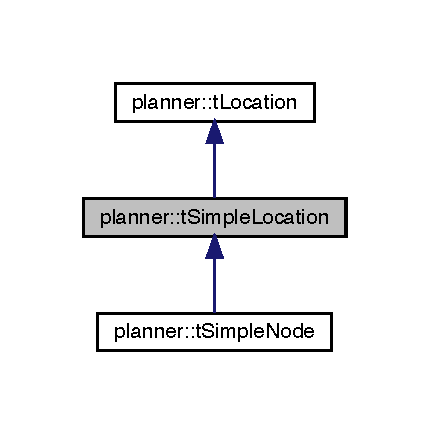
\includegraphics[width=206pt]{structplanner_1_1t_simple_location__inherit__graph}
\end{center}
\end{figure}


Collaboration diagram for planner\+:\+:t\+Simple\+Location\+:
\nopagebreak
\begin{figure}[H]
\begin{center}
\leavevmode
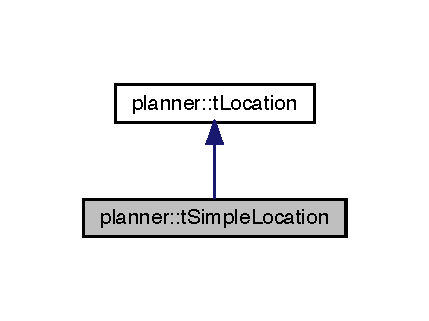
\includegraphics[width=206pt]{structplanner_1_1t_simple_location__coll__graph}
\end{center}
\end{figure}
\subsection*{Public Member Functions}
\begin{DoxyCompactItemize}
\item 
\mbox{\Hypertarget{structplanner_1_1t_simple_location_a5d8f6cbf74298ad6e80ac04f8155ece2}\label{structplanner_1_1t_simple_location_a5d8f6cbf74298ad6e80ac04f8155ece2}} 
{\bfseries t\+Simple\+Location} (int i\+\_\+n\+Id=0, int i\+\_\+nX=0, int i\+\_\+nY=0)
\item 
\mbox{\Hypertarget{structplanner_1_1t_simple_location_afa78b07e810b294b1cfd1a81379a92d3}\label{structplanner_1_1t_simple_location_afa78b07e810b294b1cfd1a81379a92d3}} 
bool {\bfseries operator$<$} (const \mbox{\hyperlink{structplanner_1_1t_simple_location}{t\+Simple\+Location}} \&i\+\_\+rhs) const
\item 
\mbox{\Hypertarget{structplanner_1_1t_simple_location_a1231d9a6478b58ed3f4c272067e67416}\label{structplanner_1_1t_simple_location_a1231d9a6478b58ed3f4c272067e67416}} 
{\footnotesize template$<$typename T\+Location $>$ }\\bool {\bfseries operator==} (const T\+Location \&i\+\_\+rhs) const
\item 
\mbox{\Hypertarget{structplanner_1_1t_simple_location_a76cc36fbdc32b448900cf5353e139dea}\label{structplanner_1_1t_simple_location_a76cc36fbdc32b448900cf5353e139dea}} 
{\footnotesize template$<$typename T\+Location $>$ }\\bool {\bfseries operator!=} (const T\+Location \&i\+\_\+rhs) const
\end{DoxyCompactItemize}
\subsection*{Public Attributes}
\begin{DoxyCompactItemize}
\item 
\mbox{\Hypertarget{structplanner_1_1t_simple_location_aa587a447cbe2af93dce4dedd14ac0b1c}\label{structplanner_1_1t_simple_location_aa587a447cbe2af93dce4dedd14ac0b1c}} 
int {\bfseries n\+Id}
\end{DoxyCompactItemize}


\subsection{Detailed Description}
Extended location struct with identifier used as hash value. 

The documentation for this struct was generated from the following file\+:\begin{DoxyCompactItemize}
\item 
/\+Users/fjp/git/bachelor/planner/include/simple\+\_\+node.\+h\end{DoxyCompactItemize}

\hypertarget{structplanner_1_1t_simple_node}{}\section{planner\+:\+:t\+Simple\+Node Struct Reference}
\label{structplanner_1_1t_simple_node}\index{planner\+::t\+Simple\+Node@{planner\+::t\+Simple\+Node}}


Simplified node struct without the a pointer to its parent as in node struct (\mbox{\hyperlink{node_8h_source}{node.\+h}}).  




{\ttfamily \#include $<$simple\+\_\+node.\+h$>$}



Inheritance diagram for planner\+:\+:t\+Simple\+Node\+:\nopagebreak
\begin{figure}[H]
\begin{center}
\leavevmode
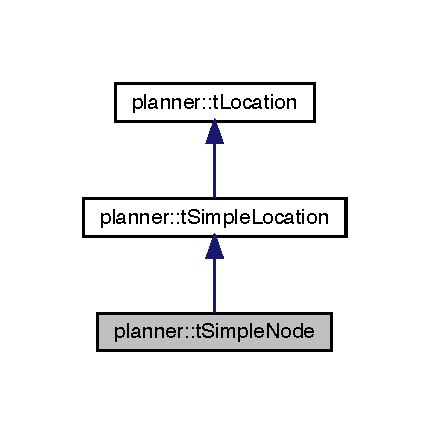
\includegraphics[width=206pt]{structplanner_1_1t_simple_node__inherit__graph}
\end{center}
\end{figure}


Collaboration diagram for planner\+:\+:t\+Simple\+Node\+:\nopagebreak
\begin{figure}[H]
\begin{center}
\leavevmode
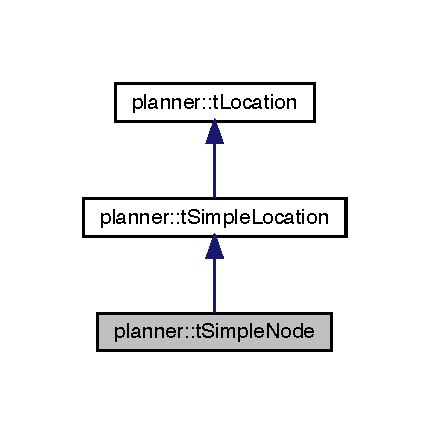
\includegraphics[width=206pt]{structplanner_1_1t_simple_node__coll__graph}
\end{center}
\end{figure}
\subsection*{Public Member Functions}
\begin{DoxyCompactItemize}
\item 
\mbox{\Hypertarget{structplanner_1_1t_simple_node_a2351b76c262d06c2a2994c2ccdc5b01c}\label{structplanner_1_1t_simple_node_a2351b76c262d06c2a2994c2ccdc5b01c}} 
{\bfseries t\+Simple\+Node} (int i\+\_\+n\+Id=0, int i\+\_\+nX=0, int i\+\_\+nY=0, double i\+\_\+g=0.\+0, double i\+\_\+h=0.\+0, double i\+\_\+f=0.\+0)
\end{DoxyCompactItemize}
\subsection*{Public Attributes}
\begin{DoxyCompactItemize}
\item 
\mbox{\Hypertarget{structplanner_1_1t_simple_node_aa75a8701dd9f556dee00365465aa21b5}\label{structplanner_1_1t_simple_node_aa75a8701dd9f556dee00365465aa21b5}} 
double \mbox{\hyperlink{structplanner_1_1t_simple_node_aa75a8701dd9f556dee00365465aa21b5}{g}}
\begin{DoxyCompactList}\small\item\em Step cost to reach this node. \end{DoxyCompactList}\item 
\mbox{\Hypertarget{structplanner_1_1t_simple_node_ae094d2027225ecdf4d5adc27177a9daa}\label{structplanner_1_1t_simple_node_ae094d2027225ecdf4d5adc27177a9daa}} 
double \mbox{\hyperlink{structplanner_1_1t_simple_node_ae094d2027225ecdf4d5adc27177a9daa}{h}}
\begin{DoxyCompactList}\small\item\em Heuristic value of this node. \end{DoxyCompactList}\item 
\mbox{\Hypertarget{structplanner_1_1t_simple_node_a3411f599ba06ac5373746571ac5223e6}\label{structplanner_1_1t_simple_node_a3411f599ba06ac5373746571ac5223e6}} 
double \mbox{\hyperlink{structplanner_1_1t_simple_node_a3411f599ba06ac5373746571ac5223e6}{f}}
\begin{DoxyCompactList}\small\item\em Combined cost of step cost and heuristic $f = g + h$. \end{DoxyCompactList}\end{DoxyCompactItemize}


\subsection{Detailed Description}
Simplified node struct without the a pointer to its parent as in node struct (\mbox{\hyperlink{node_8h_source}{node.\+h}}). 

The documentation for this struct was generated from the following file\+:\begin{DoxyCompactItemize}
\item 
/\+Users/fjp/git/bachelor/planner/include/simple\+\_\+node.\+h\end{DoxyCompactItemize}

%--- End generated contents ---

% Index
\backmatter
\newpage
\phantomsection
\clearemptydoublepage
\addcontentsline{toc}{chapter}{Index}
\printindex

\end{document}
